\documentclass[times, utf8, diplomski]{fer}
\usepackage{booktabs}
\usepackage[croatian]{babel}
\usepackage{tabularray}

\usepackage{listings}
\usepackage{color}
\usepackage{adjustbox}

\usepackage{algorithmic}
\usepackage{algorithm}

\definecolor{dkgreen}{rgb}{0,0.6,0}
\definecolor{gray}{rgb}{0.5,0.5,0.5}
\definecolor{mauve}{rgb}{0.58,0,0.82}
\definecolor{punctuation}{rgb}{0.56,0,0.14}

\lstdefinelanguage{json}{
	basicstyle=\normalfont\ttfamily,
	showstringspaces=false,
	breaklines=true,
	literate=
	*{0}{{{\color{red}0}}}{1}
	{1}{{{\color{red}1}}}{1}
	{2}{{{\color{red}2}}}{1}
	{3}{{{\color{red}3}}}{1}
	{4}{{{\color{red}4}}}{1}
	{5}{{{\color{red}5}}}{1}
	{6}{{{\color{red}6}}}{1}
	{7}{{{\color{red}7}}}{1}
	{8}{{{\color{red}8}}}{1}
	{9}{{{\color{red}9}}}{1}
	{:}{{{\color{punctuation}:}}}{1}
	{,}{{{\color{punctuation},}}}{1}
	{\{}{{{\color[rgb]{0.13,0.55,0.13}\{}}}{1}
	{\}}{{{\color[rgb]{0.13,0.55,0.13}\}}}}{1}
	{[}{{{\color[rgb]{0.13,0.55,0.13}[}}}{1}
	{]}{{{\color[rgb]{0.13,0.55,0.13}]}}}{1},
}

\lstdefinelanguage{yaml}{
	keywords={true,false,null,y,n},
	keywordstyle=\color{blue}\bfseries,
	basicstyle=\ttfamily\small,
	sensitive=false,
	comment=[l]{\#},
	commentstyle=\color{gray}\ttfamily,
	stringstyle=\color{red}\ttfamily,
	morestring=[b]',
	morestring=[b]"
}


\begin{document}

\thesisnumber{52}

\title{Analiza dnevničkih zapisa raspodijeljenih sustava u stvarnom vremenu}

\author{Matej Čubek}

\maketitle

% Dodavanje zahvale ili prazne stranice. Ako ne želite dodati zahvalu, naredbu ostavite radi prazne stranice.
\zahvala{}

\renewcommand{\lstlistingname}{Isječak koda}% Listing -> Algorithm
\renewcommand{\lstlistlistingname}{Indeks isječka kodova}% List of Listings -> List of Algorithms


\tableofcontentsƒ


\begingroup
\renewcommand*\listfigurename{Indeks slika}
\renewcommand*\listtablename{Indeks tablica}

\listoffigures

\listoftables

\endgroup

\chapter{Uvod}

Informacijski sustavi s vremenom postaju složeniji te su samim time izazovniji u pogledu održavanja i nadzora. U svijetu složenih informatičkih sustava dnevnički zapisi imaju ključnu ulogu u praćenju i održavanju kvalitete svih aplikacija. Međutim, u okruženju raspodijeljenih sustava, gdje su aplikacije pokrenute na različitim čvorovima računalnih grozdova ili računalima, pregledavanje dnevničkih zapisa svih servisa postaje iznimno zahtjevan zadatak. Ova teza, pod nazivom \emph{\glqq Analiza dnevničkih zapisa raspodijeljenih sustava u stvarnom vremenu\grqq}, proučava upotrebu \emph{Apache Kafka} platforme, \emph{ELK} platforme i \emph{OpenAI API-ja} za obradu i analizu dnevničkih zapisa raspodijeljenih sustava u stvarnom vremenu.\\

Nadzor nad dnevničkim zapisima omogućuje otkrivanje anomalija, detektiranje negativnih učinaka na performanse i drugih problema koji mogu utjecati na kvalitetu usluge. Cilj je ove teze istražiti mogućnosti Kafka platforme za analizu dnevničkih zapisa, s posebnim naglaskom na detekciju i nadzor anomalija u raspodijeljenim sustavima.

Ovaj rad proučavat će Apache Kafka  i ELK platforme istražujući kako se mogu koristiti za obradu i analizu dnevničkih zapisa u stvarnom vremenu. Analiza će se napraviti na stvarnom primjeru SaaS-a\footnote{Softver kao usluga \engl{Software as a Service}} \emph{CloudVane} tvrtke \emph{Neos} te će se upravo na toj distribuiranoj aplikaciji pokazati iskoristivost rješenja rada.

Također, rad će razmatrati kako se korištenim alatima mogu poboljšati pouzdanost i brzina obrade podataka kako bi se pravovremeno moglo odazvati na probleme sustava. Očekuje se da će ovaj rad pružiti dublje razumijevanje važnosti i mogućnosti analize dnevničkih zapisa u raspodijeljenim sustavima, kao i uloge Kafka platforme u tom kontekstu.\\

Poglavlje \ref{sec:app_arch} početak je ovog rada i pruža uvid u arhitekture aplikacija, uz opis monolitnih i distribuiranih aplikacija, kao i metoda njihovih implementiranja. Nadalje, poglavlje \ref{sec:cloudvane} posvećeno je CloudVane aplikaciji, njenim komponentama kao što su Apache Kafka i Kubernetes. U poglavlju \ref{sec:monitoring} izloženo je kako se vrši nadzor putem dnevničkih zapisa i objašnjena je upotreba ELK platforme. Poglavlje \ref{sec:streamingMonitoring} opisuje proces obrade dnevničkih zapisa u stvarnom vremenu. Završno, poglavlje \ref{sec:conclusion} donosi rezime i osvrt na sve što je istraženo i predstavljeno u ovom radu.

\chapter{Arhitektura aplikacija}
\label{sec:app_arch}

Prvobitno su se računalne aplikacije pokretale na izoliranim serverima, svaki posvećen isključivo posluživanju jedne aplikacije. Ova je arhitektura omogućavala da svaka aplikacija ima svoje računalo na kojem radi, često smješteno u posebnoj server-sali ili odvojenoj sobi. Ovaj pristup bio je jednostavan i lako razumljiv, te je omogućavao izravno mapiranje između aplikacija i odgovarajućih resursa. 

No, ovaj model nije bio bez ograničenja. Prvo, to je stvorilo nedostatak fleksibilnosti u pogledu alokacije resursa jer su se resursi često prekomjerno koristili za jednu aplikaciju, dok su ostale aplikacije patile od nedostatka resursa. Budući da svaka aplikacija zahtijeva svoj vlastiti fizički server, ovaj pristup bio je neučinkovit u pogledu prostora i energije.

Uz to, održavanje takvih izoliranih sustava predstavljalo je izazov. Svaki server morao se održavati odvojeno, što je uključivalo nadogradnje hardvera, instalacije softvera, popravke i slično. Također, ovaj model nije pružao adekvatnu otpornost na kvarove --- ako bi server prestao raditi, cijela bi aplikacija bila nedostupna sve dok se server ne popravi ili zamijeni, što može rezultirati značajnim prekidima u radu.
Stoga su se s vremenom razvile nove arhitekture, poput distribuiranih sustava i virtualizacije, koje su omogućile fleksibilniju, učinkovitiju i otporniju upotrebu računalnih resursa.\\

U ovom će se poglavlju razmotriti različite arhitekture aplikacija, uključujući distribuirane i monolitne sustave te različite metode njihove implementacije.


\section{Monolitne aplikacije}
\label{sec:monolith}

\textbf{Monolitne aplikacije} karakterizira integracija svih funkcionalnosti unutar jedinstvene operativne jedinice. U ovakvom sustavu sve komponente, od korisničkog sučelja do pozadinskog sustava i baze podataka, tvore koherentnu cjelinu iste aplikacije. \\

Glavna prednost monolitne arhitekture leži u njenom centraliziranom pristupu koji pojednostavljuje interakcije među komponentama eliminirajući potrebu za kompleksnom komunikacijom koja je česta kod distribuiranih aplikacija. Osim toga, monolitne aplikacije često su jednostavnije za testiranje i održavanje jer se ne zahtijeva upravljanje mnoštvom odvojenih servisa. 

Ipak, monolitne aplikacije imaju nedostatke. Jedan je od ključnih izazova skaliranje: kako raste opterećenje na aplikaciju, monolitne aplikacije omogućavaju samo vertikalno skaliranje, što znači povećanje resursa na postojećem serveru. Horizontalno skaliranje, koje podrazumijeva dodavanje dodatnih servera, nije moguće. Također, ažuriranje ili mijenjanje bilo kojeg segmenta aplikacije često zahtijeva ponovnu implementaciju \engl{deployment} cijelog sustava, što može dovesti do privremene nedostupnosti usluge. \\

Unatoč ovim izazovima, monolitne aplikacije zadržavaju značajnu prisutnost u računalnoj industriji. U mnogim ih slučajevima njihova jednostavnost, kombinirana s potencijalnom uštedom u mrežnom prometu, čini atraktivnom opcijom za manje složene i manje opterećene sustave.


\section{Distribuirane aplikacije}
\label{sec:distributed}

\textbf{Distribuirane ili raspodijeljene} aplikacije predstavljaju temelj suvremenih informacijskih sustava i usluga koje se svakodnevno koriste. Ove aplikacije koriste se u različitim industrijama i sektorima, od financija, zdravstva, obrazovanja, pa sve do zabave i medija. Njihova je osnovna značajka sposobnost paralelne obrade podataka na više računalnih čvorova i geografskih lokacija, čime se omogućuje brza i pouzdana usluga bez obzira na fluktuacije u potražnji. Dodatno, distribuirani sustav je skup neovisnih računala koji korisniku izgleda kao jedan cjeloviti sustav \citep{tanenbaum_distributed_2007}.\\

Pokretanje aplikacija na različitim računalnim čvorovima znači da instance aplikacije mogu podijeliti opterećenje povećavajući tako učinkovitost i performanse sustava. Ova decentralizacija također znači da kvar jednog čvora neće onemogućiti rad cijele aplikacije. Umjesto toga, rad će biti preusmjeren na ostale čvorove osiguravajući tako kontinuitet usluge. Upravo je ta visoka dostupnost, robusnost i brzina odziva ključna prednost distribuiranih aplikacija. Uz to, fleksibilnost skaliranja omogućuje im da se prilagode promjenjivim uvjetima potražnje, dodavanjem ili uklanjanjem računalnih čvorova prema potrebi.

No, unatoč brojnim prednostima, distribuirane aplikacije donose i određene izazove. \citet{zarko_raspodijeljeni_2013} navodi kako složena pitanja poput koordinacije i sinkronizacije među čvorovima, očuvanje konzistencije podataka kroz različite komponente sustava te upravljanje povećanim složenostima mreže zahtijevaju sofisticirane strategije i tehnike. Algoritmi i protokoli za rješavanje ovih problema moraju biti pažljivo osmišljeni kako bi se osigurao pravilan rad distribuiranog sustava. \\

Unatoč ovim izazovima, distribuirane aplikacije ostaju ključan alat za postizanje visoke efikasnosti, pouzdanosti i fleksibilnosti u današnjem digitalno povezanom svijetu. Budući da tehnologija napreduje, distribuirane aplikacije postaju sve sofisticiranije, pružajući sve naprednija rješenja za suvremene poslovne i društvene izazove.

\subsection{Mikro-servisne aplikacije}
\label{sec:microservices}

Aplikaciju \textbf{mikro-servisne} arhitekture \engl{microservice architecture} čini kolekcija malih autonomnih servisa. Svaki servis ima svoje funkcionalnosti, no uz međusobnu komunikaciju stvaraju kohezivnu cjelinu.

Na slici \ref{fig:microservice} može se vidjeti kako mikro-servisna arhitektura izgleda u usporedbi s monolitnom arhitekturom opisanom u poglavlju \ref{sec:monolith}. Iako mikro-servisna arhitektura donosi izazove poput složenije komunikacije i održavanja sinkronizacije podataka, istovremeno pruža znatne prednosti, kao što su pojednostavljeno horizontalno skaliranje i smanjeni rizik od sistemskih kvarova zahvaljujući autonomiji servisa.
Radi efikasnosti u radu s mikro-servisima često se koristi kontejnerizacija, opisana u poglavlju \ref{sec:docker}, i  orkestracijski alati poput Kubernetes-a opisanog u poglavlju \ref{sec:k8s}. Upravo takav sustav koristi aplikacija CloudVane opisana u poglavlju \ref{sec:cloudvane} na čijim se dnevničkim zapisima bazira ovaj rad.

\begin{figure}[htb]
	\centering
	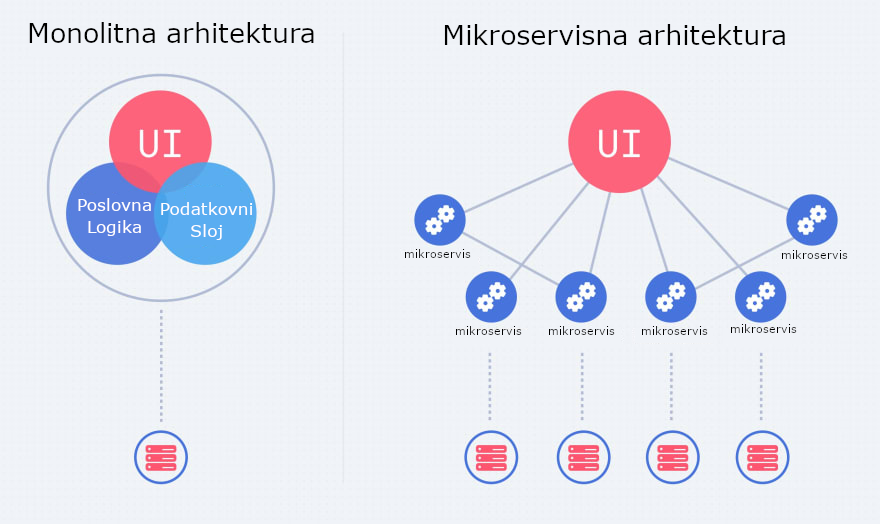
\includegraphics[width=15cm]{images/microservice.png}
	\caption[Usporedba monolitne arhitekture s mikro-servisnom arhitekturom]{Usporedba monolitne arhitekture s mikro-servisnom arhitekturom\\Slika preuzeta sa \url{https://dev.to/alex_barashkov/microservices-vs-monolith-architecture-4l1m}}
	\label{fig:microservice}
\end{figure}


\section{Pokretanje direktno na hardveru računala}

Pokretanje na hardveru \engl{bare metal} znači da se aplikacije izvršavaju na namjenskom računalu, bez upotrebe virtualizacije. Ovakva konfiguracija omogućuje korištenje svih raspoloživih resursa računala, poput procesorske snage, memorije i prostora za pohranu. \\

Primjena ovog pristupa donosi niz prednosti poput boljih performansi zbog izravnog pristupa hardveru, bez posredničkog sloja koji donosi dodatno opterećenje \engl{overhead}. Dodatno, pokretanje na namjenskom hardveru može pružati i veću sigurnost jer se eliminiraju rizici dijeljenja resursa s drugim aplikacijama.

Upravljanje hardverom međutim može uzrokovati složenije i vremenski zahtjevnije procese, posebno kada je riječ o održavanju. Skaliranje aplikacija također predstavlja izazov jer zahtijeva nabavku novog hardvera i migraciju aplikacija na nove resurse.

Unatoč tim izazovima, aplikacije koje zahtijevaju visoko-intenzivne resurse mogu značajno profitirati od prednosti koje pruža ovaj pristup. Pokretanje aplikacija na samom hardveru usporedno s virtualnim strojevima i kontejnerima opisanim kasnije prikazano je na slici \ref{fig:infra}\footnote{Kernel je glavni program operacijskog sustava, a Hypervisor je program koji upravlja virtualnim strojevima.}.

\begin{figure}[htb]
	\centering
	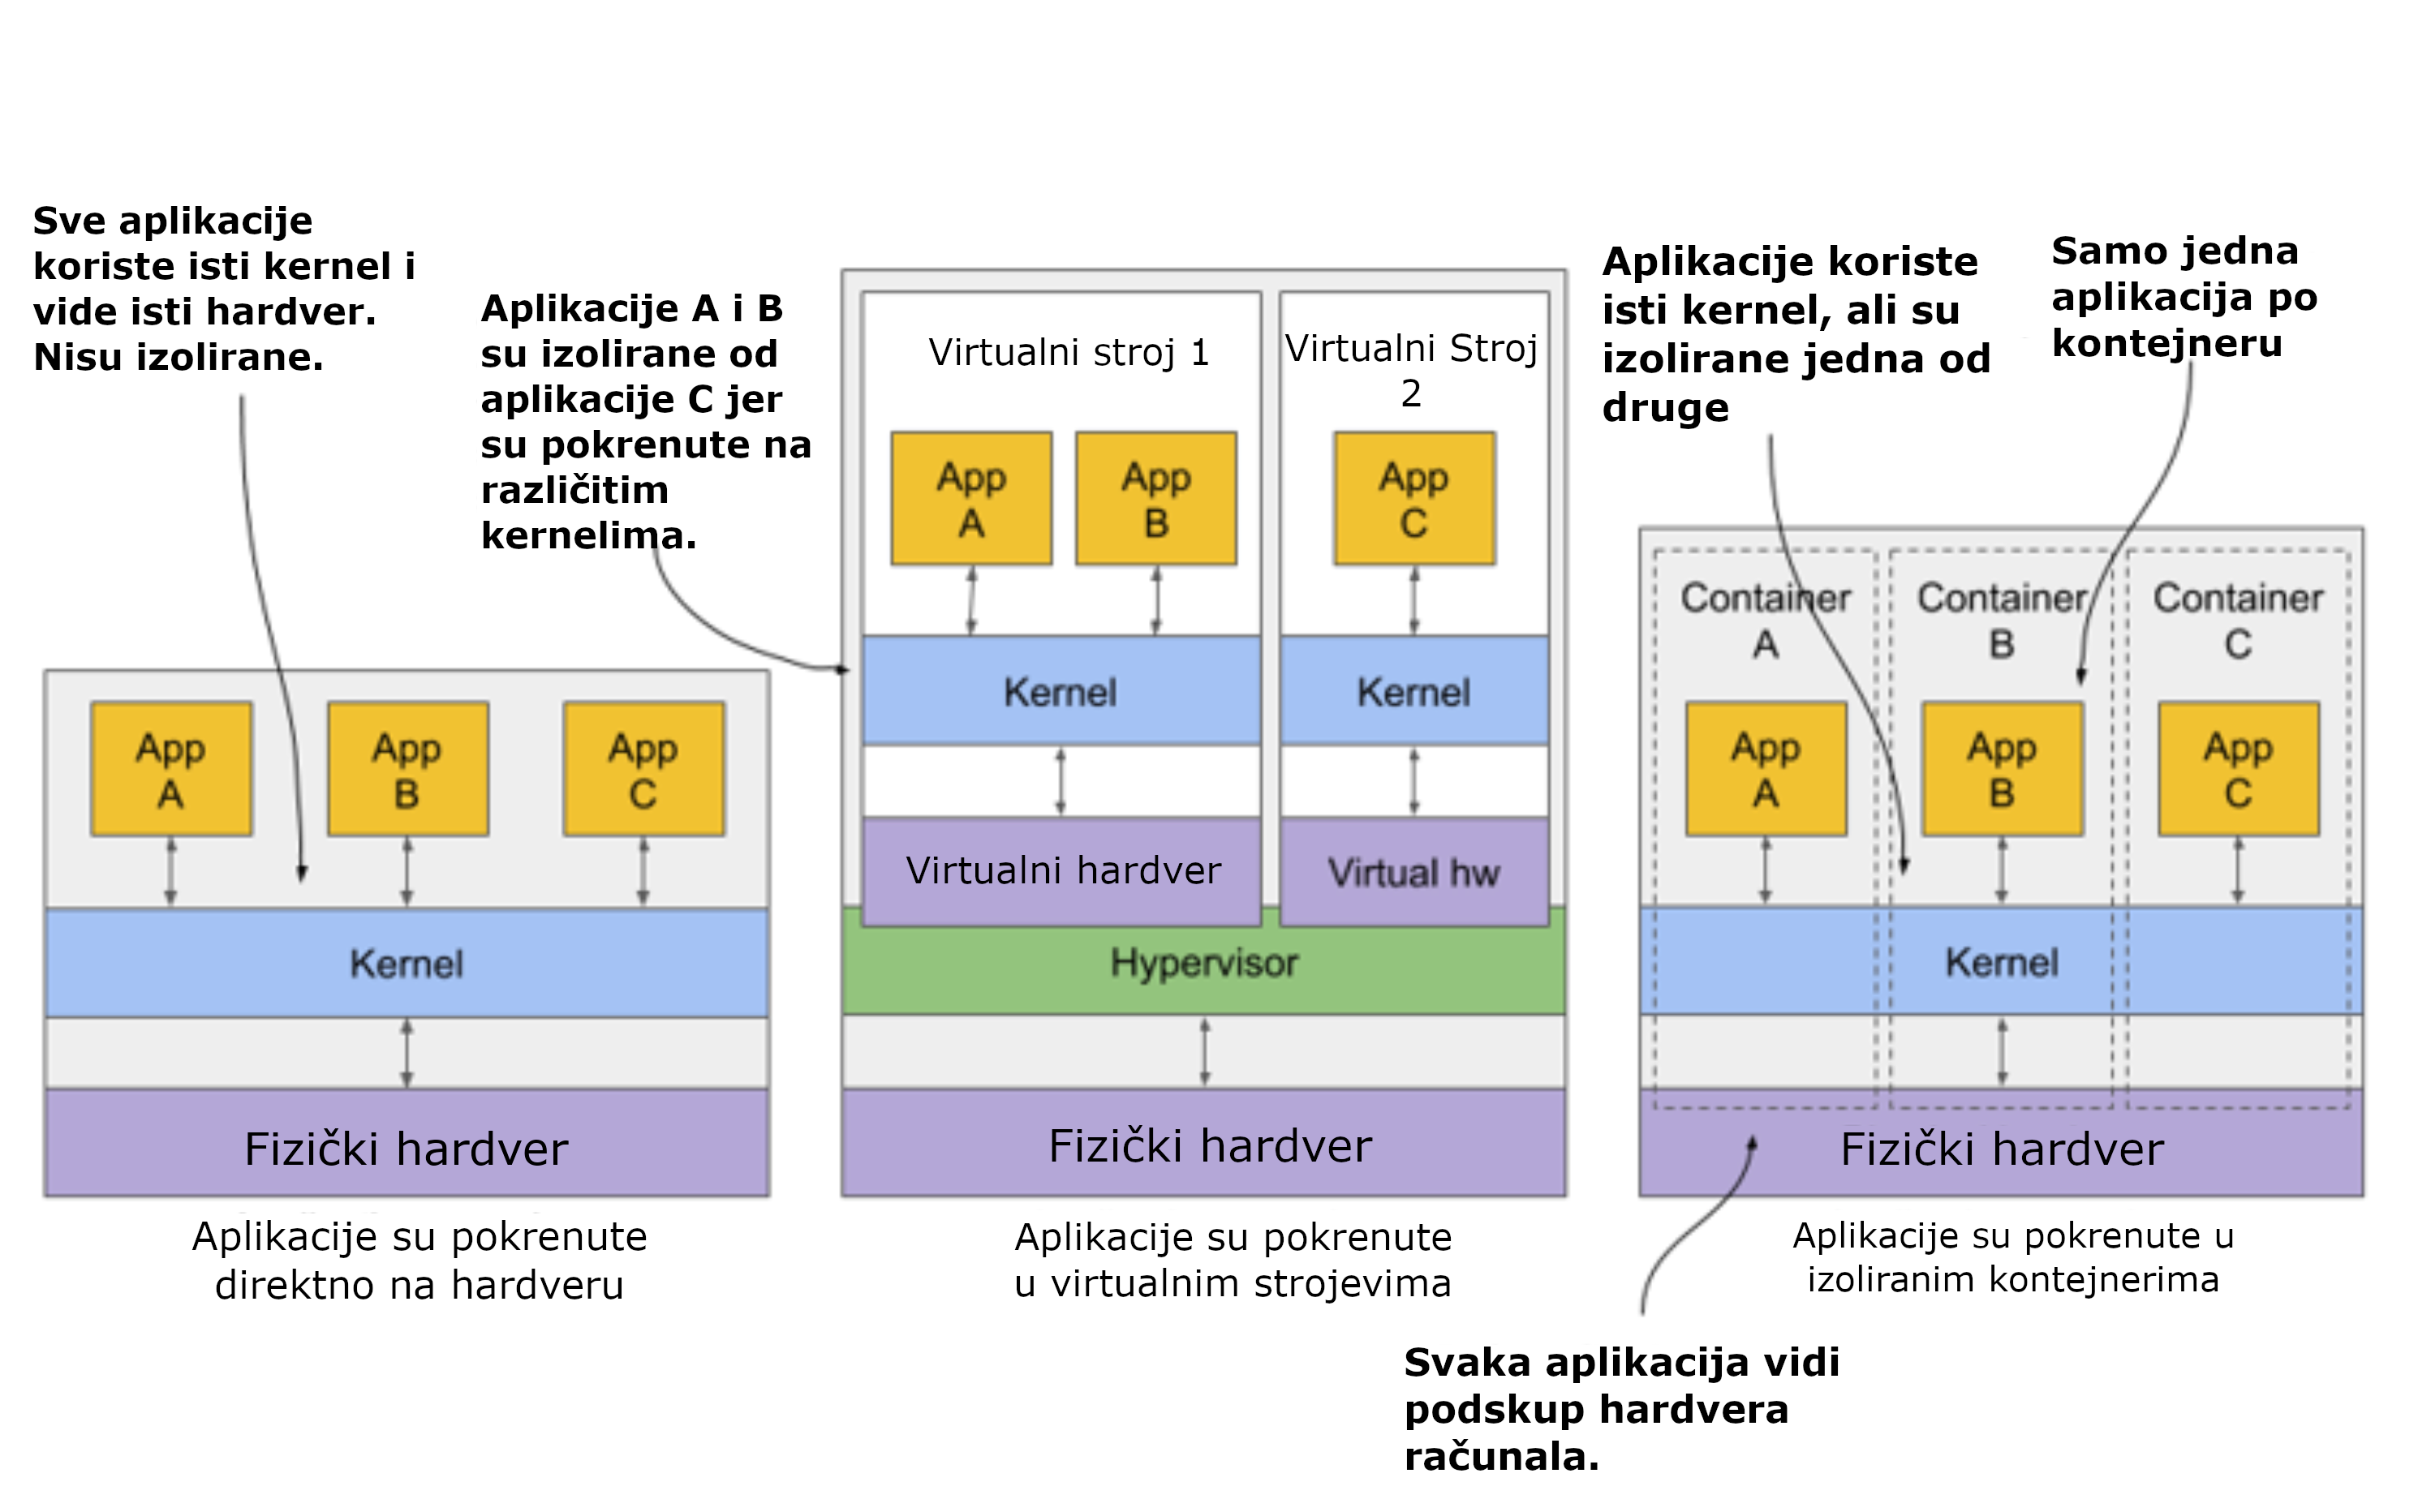
\includegraphics[width=15cm]{images/infra.png}
	\caption[Usporedba pokretanja direktno na hardveru, virtualnim strojevima i kontejnerima]{Usporedba pokretanja direktno na hardveru, virtualnim strojevima i kontejnerima\\Slika preuzeta iz \emph{Lukša, M. (2023). Kubernetes in Action, Second Edition. (n.p.): Manning.}}
	\label{fig:infra}
\end{figure}

\section{Virtualni strojevi}

\textbf{Virtualni strojevi} \engl{Virtual Machine} su sofisticirani koncept koji simulira hardver kroz softver. Oni predstavljaju sloj apstrakcije između aplikacije i fizičkog hardvera na kojem se izvršava. Aplikacija se prividno izvršava na vlastitom, nezavisnom sustavu. \\

Korištenje virtualnih strojeva donosi niz značajnih prednosti. Prva među njima je mogućnost učinkovitijeg iskorištavanja računalnih resursa. Na jednom fizičkom računalu moguće je pokrenuti nekoliko virtualnih strojeva, svaki sa svojim operativnim sustavom i aplikacijama, čime se maksimizira iskorištavanje hardverskih resursa i smanjuje potreba za nabavom dodatnog hardvera.

Još jedan bitan aspekt korištenja virtualnih strojeva je izolacija. S obzirom na to da su virtualni strojevi nezavisne jedinice, moguće je pokrenuti različite aplikacije na različitim operativnim sustavima na istom fizičkom računalu. Ova izolacija smanjuje rizik od međusobnog utjecaja aplikacija i povećava sigurnost jer potencijalni problemi ili napadi na jedan virtualni stroj ne utječu na drugi.

Uz to, virtualni strojevi pružaju veliku fleksibilnost i skalabilnost. Dodavanje ili uklanjanje virtualnih strojeva, prema potrebama korisnika ili aplikacije, može se obaviti brzo i efikasno. Mogućnost preslikavanja \engl{snapshotting} i kloniranja virtualnih strojeva olakšava sigurnosne kopije \engl{backup} i oporavak sustava te omogućava jednostavno testiranje i razvoj.

Međutim, unatoč brojnim prednostima, korištenje virtualnih strojeva donosi i određeno dodatno opterećenje \engl{overhead}. Svaki virtualni stroj zahtijeva određeni dio računalnih resursa za rad operativnog sustava, što može rezultirati manjom efikasnošću u odnosu na pokretanje aplikacija direktno na hardveru. Upravljanje velikim brojem virtualnih strojeva također može biti složeno, ali postoje različiti alati i platforme za upravljanje virtualnim okruženjima koji mogu pomoći u tome. Usporedba pokretanja na virtualnim strojevima s pokretanjem direktno na hardveru i kontejnerima objašnjenim u sljedećem poglavlju vidljiva je na slici \ref{fig:infra}.

\section{Kontejnerizacija i Docker}
\label{sec:docker}

\textbf{Kontejnerizacija} \engl{containerization} je proces pakiranja aplikacije zajedno s potrebnim okruženjem i zavisnostima \engl{dependencies}, što omogućuje jednostavno izvršavanje i pokretanje aplikacije u različitim računalnim okruženjima. Kontejneri su izolirane jedinice koje sadrže sve što je potrebno za izvršavanje aplikacije uključujući programski kod, izvršno okruženje \engl{runtime}, sistemske alate, knjižnice \engl{libraries} i postavke. \\

\textbf{Docker} je najpoznatiji alat za kontejnerizaciju koji je postao standard u industriji. S Dockerom programeri mogu stvoriti, pokrenuti i distribuirati aplikacije unutar kontejnera. Kontejneri stvoreni pomoću Dockera\footnote{Kroz Docker je moguće pokrenuti kontejnere koje su kreirali različiti alati, pod uvjetom da implementiraju Open Container Initiative standard koji je postavila Linux Fundacija. Slično tome, kontejneri koji su kreirani korištenjem Dockera mogu se pokrenuti kroz bilo koje drugo izvršno okruženje kontejnera koje podržava Open Container Initiative. Ova interoperabilnost omogućava veću fleksibilnost i slobodu izbora prilikom rada s kontejnerima.} mogu se pokrenuti bilo gdje je Docker instaliran bez obzira na osnovni operativni sustav. To znači da programeri ne moraju brinuti o kompatibilnosti operativnih sustava prilikom pokretanja svojih aplikacija.

Kontejnerizacija donosi brojne prednosti. Kontejneri su manji i brži od tradicionalnih virtualnih strojeva jer ne zahtijevaju cijeli operativni sustav. Osim toga, kontejneri osiguravaju konzistentnost okruženja kroz razne faze razvojnog ciklusa aplikacija. Uz to, Docker omogućuje jednostavno skaliranje aplikacija dodavanjem ili uklanjanjem kontejnera po potrebi.

Kao rezultat, kontejnerizacija i Docker postali su ključni elementi modernih razvojnih ciklusa i \emph{DevOps}\footnote{DevOps je skup praksi, filozofija i alata koji poboljšavaju suradnju između razvoja softvera \engl{Dev} i IT operacija \engl{Ops}} praksi, igrajući ključnu ulogu u povećanju efikasnosti i brzine isporuke softvera. 

Usporedba kontejnera, koji su zahvaljujući svojim prednostima postali temelj sustava poput \emph{Kubernetes} iz poglavlja \ref{sec:k8s}, s pokretanjem direktno na hardveru i virtualnim strojevima prikazana je na slici \ref{fig:infra}.

\section{Računarstvo u Oblaku}

\textbf{Računarstvo u oblaku} \engl{Cloud computing} koncept je pružanja IT\footnote{Informatička Tehnologija \engl{Information Technology}} usluga u kojem se resursi poput računalne snage, prostora za pohranu, aplikacije i drugi resursi pružaju kroz internet na zahtjev korisnika ovisno o njegovoj potrebi \citep{zarko_raspodijeljeni_2013}. Oblak omogućuje korisnicima da ne moraju upravljati računalnim resursima, već njima upravlja pružatelj usluga oblaka. \\

Prednosti oblaka uključuju fleksibilnost, skalabilnost i troškovnu učinkovitost. Fleksibilnost dolazi od sposobnosti korisnika da brzo i jednostavno prilagode svoje resurse u skladu s potrebama. Skalabilnost se odnosi na mogućnost dodavanja ili uklanjanja resursa u skladu s promjenama u potražnji. Troškovnu učinkovitost omogućuje model u kojem korisnici plaćaju samo za resurse koje koriste.

Prema \citet{zarko_raspodijeljeni_2013} postoje različiti modeli oblaka:
\begin{description}
	\item [Javni oblak:] pružatelj usluga resurse pruža svim korisnicima preko interneta.
	\item [Privatni oblak:] infrastruktura posvećena samo jednoj organizaciji.
	\item [Hibridni oblak:] mješavina javnog i privatnog oblaka, pruža organizacijama veću fleksibilnost prilikom upravljanja svojim resursima.
\end{description}

Korištenje usluga u oblaku također omogućava pristup naprednim tehnologijama i alatima, poput orkestracije kontejnera, automatizacije, umjetne inteligencije i analiza podataka, koje bi bile teško dostupne ili skupe za implementaciju na vlastitoj infrastrukturi.

Osim toga, pružatelji usluga u oblaku nude sofisticirane mehanizme sigurnosti, otpornosti na pogreške i oporavka podataka, čime dodatno povećavaju dostupnost i pouzdanost aplikacija koje se nalaze u oblaku.

\subsection{Grozdovi računala}

\textbf{Grozdovi računala ili klasteri} \engl{clusters} predstavljaju skupinu povezanih računala koja rade zajedno na takav način da se u mnogim aspektima mogu smatrati jedinstvenim sustavom \citep{zarko_raspodijeljeni_2013}. Grozdovi računala omogućuju paralelnu obradu zadataka, visoku dostupnost usluga, ravnomjerno opterećenje i skalabilnost.

Jedna od ključnih prednosti grozdova računala je visoka dostupnost usluga zahvaljujući mogućoj distribuciji zadataka. Kao što je navedeno u poglavlju \ref{sec:distributed}, u slučaju kvara jednog računala, ostala računala u klasteru mogu preuzeti njegove zadatke i osigurati neprekidno pružanje usluga. To je posebno korisno za aplikacije i usluge koje zahtijevaju kontinuiranu dostupnost.

Grozdovi računala, zahvaljujući distribuiranosti, također omogućuju paralelnu obradu podataka, gdje se kompleksni zadaci mogu podijeliti na manje dijelove koje svako računalo u klasteru obrađuje istovremeno. To može značajno smanjiti vrijeme potrebno za obradu velikih količina podataka.

Unatoč svim prednostima, upravljanje grozdovima računala može biti složeno i zahtijeva adekvatne alate i stručnost. Moraju se uspostaviti mehanizmi za koordinaciju između računala, ravnomjerno raspoređivanje opterećenja, otkrivanje i oporavak od kvarova te osiguravanje konzistentnosti podataka. \\

U kontekstu grozdova računala \emph{Računalni oblak} \engl{Cloud} pruža ključnu infrastrukturu koja značajno olakšava upravljanje. Koristeći oblak, organizacije se mogu fokusirati na razvoj i izvršavanje svojih aplikacija bez potrebe za postavljanjem i održavanjem vlastite hardverske infrastrukture.

Pružatelji usluga u oblaku, poput \emph{Amazon Web Services} (\textbf{AWS}), \emph{Google Cloud Platform} (\textbf{GCP}), \emph{Microsoft Azure} ili \emph{Oracle Cloud Infrastructure} (\textbf{OCI}), nude usluge za upravljanje grozdovima računala koje olakšavaju postavljanje, skaliranje i održavanje. Ti se grozdovi mogu lako prilagoditi potrebama korisnika, bilo da je riječ o povećanju ili smanjenju broja računala u grozdu.

\subsection{Lambda funkcije}

\textbf{Lambda funkcije}, koje su popularizirane kroz računalni oblak \textbf{AWS}\footnote{Amazon Web Services}, predstavljaju ključni dio koncepta \textbf{bez-servernog} \engl{serverless} računarstva. Naziv potječe od koncepta da se programeri ne trebaju brinuti o infrastrukturi na kojoj se njihova usluga pokreće.

Lambda funkcije esencijalno su blokovi koda koji su dizajnirani za obavljanje specifične zadaće i koji se mogu pokrenuti na zahtjev. One se izvršavaju samo kada su potrebne, što znači da korisnici plaćaju samo za vrijeme izvršavanja koda, a ne za stalno prisutne poslužitelje.

Budući da AWS automatski dodjeljuje potrebne resurse za izvršavanje funkcije, bez obzira na to je li potrebno pokrenuti jednu instancu ili tisuće instanci, ove funkcije omogućuju iznimnu skalabilnost. Lambda funkcije mogu se koristiti za različite zadatke, uključujući obradu podataka u stvarnom vremenu, automatizaciju zadataka, pa čak i izgradnju cijelih mikro-servisnih aplikacija. \\

Unatoč prednostima koje nude mikro-servisi i bez-serverna \engl{serverless} arhitektura kao što su fleksibilnost i mogućnost neovisnog skaliranja komponenti, studija provedena u sklopu članka \citet{kolny_scaling_2023} pokazuje da ove prednosti ne dolaze bez troškova. U slučaju \emph{Amazon Prime Video} originalna se arhitektura usluge za nadzor audio/video sadržaja temeljila na distribuiranom modelu mikro-servisa, koji je uključivao AWS Lambda funkcije. Međutim, ova arhitektura pokazala se skupom i s ograničenjima skaliranja.

Kako bi riješio ove probleme, Amazon Prime Video je rekonstruirao uslugu u monolitnu aplikaciju, što je rezultiralo značajnim smanjenjem infrastrukturnih troškova --- čak $90\%$. Ova promjena eliminirala je potrebu za skupim prijenosima podataka između distribuiranih komponenti i pojednostavila logiku orkestracije.

\citet{kolny_scaling_2023} naglašava važnost pažljivog razmatranja pri odabiru arhitekture. Govori kako mikro-servisi i Lambda funkcije mogu pružiti visoku razinu fleksibilnosti, mogu također donijeti značajne troškove i ograničenja skaliranja. Stoga u nekim slučajevima, kao što je ovaj, monolitna arhitektura može biti isplativija opcija.



\chapter{Distribuirana aplikacija --- CloudVane}
\label{sec:cloudvane}

\textbf{CloudVane} je proizvod koji pomaže upravljati i optimizirati trošak te infrastrukturu u \emph{više-oblačnom} \engl{multicloud} okruženju  \citep{neos_cloudvane_2023}. Glavni je cilj CloudVane aplikacije pružiti vidljivost i kontrolu nad upotrebom oblaka \engl{clouda} u cijeloj organizaciji. \\

CloudVane je izgrađen na \textbf{FinOps}\footnote{FinOps je udruga koja se bavi kulturom upravljanja troškova usluga u oblaku. Naziv FinOps dolazi od riječi financijsko upravljanje \engl{Financial Operations} i definira prakse, principe i kulturu kako bi organizacije bolje razumjele svoje troškove u oblaku i donosile informirane poslovne odluke \citep{finops_fundation_finops_nodate}.} principima koji se fokusiraju na razumijevanje i upravljanje troškovima u oblaku i resursima kako bi se donijele informirane poslovne odluke. CloudVane sadrži alatnu ploču \engl{dashboard} koja nudi pogled na izvještaje iz oblaka, proračune, pragove proračuna i hijerarhiju organizacije kroz jedinstveni pogled.
Neke od funkcionalnosti koje CloudVane nudi jesu:

\begin{itemize} 
\item preporuke za pravilno dimenzioniranje\footnote{Dimenzioniranje je skaliranje resursa na oblaku s obzirom na njihovu stvarnu potrošnju kako bi se smanjila neiskorištenost.}
\item uvidi u uporabu resursa
\item otkrivanje anomalija u troškovima
\item planiranje rezerviranih instanci\footnote{Rezervirane instance \engl{Reserved instances} jesu unaprijed plaćene usluge oblaka s popustom.}.
\item izvještaji o uštedama oblaka i resursa
\item automatizacije nad resursima\footnote{Automatizacije čine gašenje resursa kada se ne koriste u svrhu uštede.}
\item obavijesti o troškovima
\end{itemize}

Upravo na primjeru distribuirane aplikacije CloudVane čija je arhitektura prikazana na slici \ref{fig:cloudvaneArch}, a protok podataka na slici \ref{fig:dataCloudvane}, ovaj rad će demonstrirati analizu dnevničkih zapisa objašnjenih u poglavlju \ref{sec:logs}, svih dostupnih mikro-servisa aplikacije CloudVane u stvarnom vremenu \engl{real-time} sa svrhom kreiranja sustava nadgledanja i nadzora aplikacija \engl{application monitoring}.

\begin{figure}[htb]
	\centering
	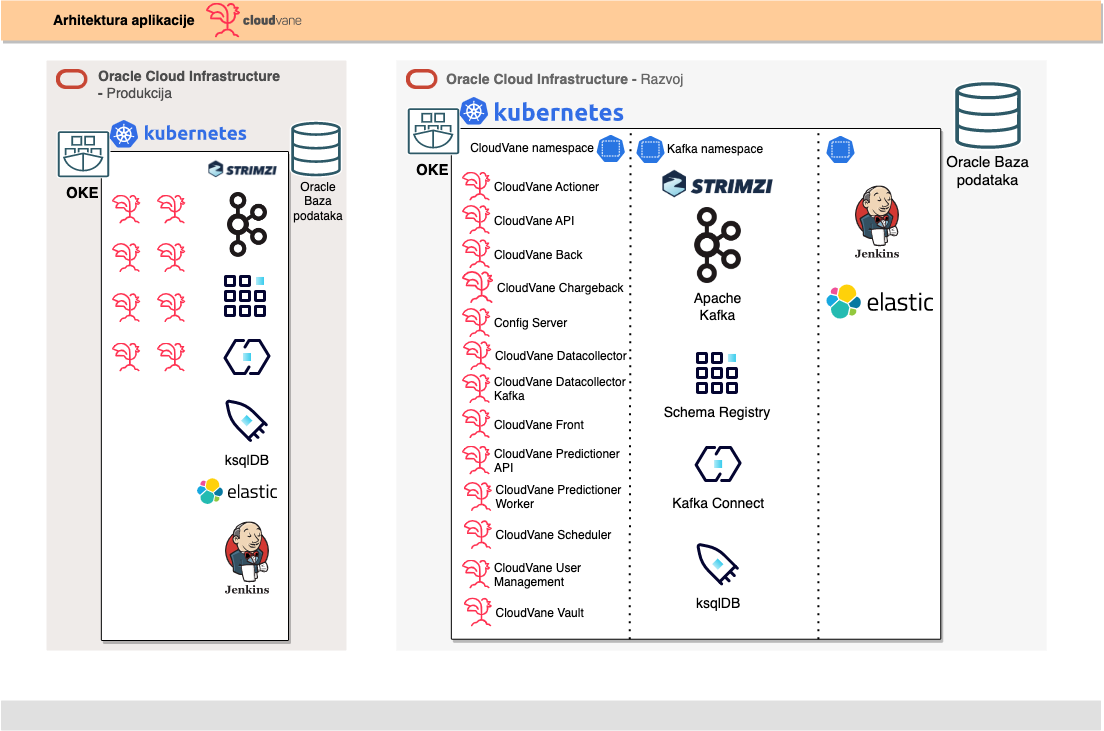
\includegraphics[width=15cm]{images/CloudVaneArchitecture.png}
	\caption[Arhitektura CloudVane sustava]{Arhitektura CloudVane sustava}
	\label{fig:cloudvaneArch}
\end{figure}

\begin{figure}[htb]
	\centering
	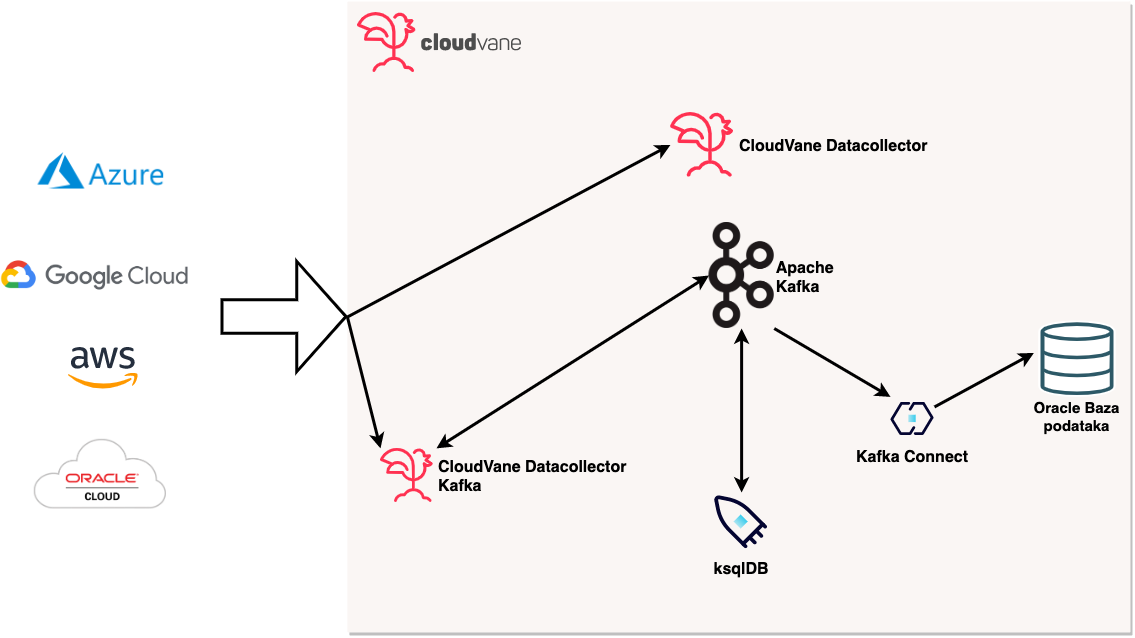
\includegraphics[width=15cm]{images/CloudVaneData.png}
	\caption[Tok podataka CloudVane sustava]{Tok podataka \engl{data pipeline} CloudVane sustava}
	\label{fig:dataCloudvane}
\end{figure}

Nadalje, CloudVane aplikacija je pokrenuta na infrastrukturi održavanog Kubernetes grozda \engl{managed Kubernetes cluster} na \emph{Oracle Cloud Infrastructure} (OCI) oblaku. \emph{Kubernetes}, opisan u poglavlju \ref{sec:k8s}, pokreće sve komponente aplikacije CloudVane koji uključuju i Apache Kafku opisanu u poglavlju \ref{sec:kafka}, osim Oracle relacijske baze podataka koja se pokreće kao servis na samom OCI oblaku. Arhitektura aplikacije opisana je u poglavlju \ref{sec:architecture}, a transparentnost koju pruža Kubernetes omogućuje selidbu cijele infrastrukture na bilo koji \emph{hiper-skalabilni pružatelj usluga oblaka}\footnote{Ovaj termin odnosi se na najveće pružatelje usluge oblaka poput Amazon Web Services (AWS), Google Cloud Platform (GCP), Microsoft Azure itd. Naziv dolazi od sposobnosti brzog skaliranja računalne infrastrukture s obzirom na potražnju.} \engl{hyperscaler}.

\clearpage
\section{Orkestrator kontejnera --- Kubernetes}
\label{sec:k8s}

\citet{luksa_kubernetes_2023} definira \textbf{Kubernetes} kao softverski sustav za automatizaciju implementacije \engl{deployment} i upravljanja složenim, velikim aplikacijskim sustavima sastavljenim od računalnih procesa koji rade u kontejnerima.
Kubernetes programerima pruža sloj apstrakcije nad hardverom, što im omogućava da se usredotoče na razvoj aplikacija umjesto na upravljanje infrastrukturom.

Tako Kubernetes omogućuje implementaciju aplikacija potpuno transparentno, bez obzira na broj čvorova grozda i njihovu arhitekturu. Programeri ne moraju brinuti o detaljima kao što su odabir hardvera, operacijskog sustava za svaki čvor ili podjela resursa između različitih aplikacija. Kubernetes također može skalirati aplikacije na temelju opterećenja i automatski se oporavlja od pogrešaka, čime se osigurava visoka dostupnost i otpornost aplikacija. Zahvaljujući tome aplikacije mogu nesmetano raditi čak i u slučaju otkazivanja hardvera ili mrežnih problema.\\

Kubernetes se može pokrenuti direktno na hardveru računala nudeći potpunu kontrolu i fleksibilnost u konfiguraciji i upravljanju resursima. Alternativno se Kubernetes može koristiti kao \emph{potpuno održavana usluga} \engl{managed service} na oblaku \engl{cloud}. Potpuno održavan Kubernetes uvelike olakšava postavljanje i upravljanje Kubernetes grozdovima preuzimajući na sebe vremenski zahtjevne operativne zadatke poput skaliranja, nadogradnje, sigurnosti i ostalog održavanja.

Bez obzira na to kako je pokrenut, Kubernetes donosi robustan, fleksibilan i skalabilan okvir za upravljanje kontejnerskim aplikacijama koji omogućuje transparentno i jednostavno upravljanje distribuiranim aplikacijama.

\subsection{Implementacija aplikacije CloudVane na Kubernetesu}

Kao što je prethodno spomenuto, svi mikro-servisi koje koristi CloudVane, kao i Apache Kafka servisi kasnije opisani u poglavlju \ref{sec:kafka}, operiraju unutar Kubernetes klastera na Oracle Cloud Infrastructure (OCI) platformi. DevOps prakse, koje kombiniraju elemente softverskog razvoja \engl{Development} i IT operacija \engl{Operations} kako bi se poboljšala brzina isporuke i kvaliteta softvera \citep{courtemanche_what_nodate}, također su implementirane unutar ovog sustava.\\

\textbf{Jenkins}, moćan alat za kontinuiranu integraciju koji automatizira ključne aspekte razvojnog procesa softvera, poput izgradnje, testiranja i implementacije koda, dodatno je integriran u ovaj Kubernetes klaster. Jenkins omogućuje korisnicima agilne DevOps procese pružajući automatizirane cikluse izgradnje za brzu i pouzdanu isporuku koda.\\

Jedini element infrastrukture koji se ne pokreće unutar Kubernetes klastera je \emph{Oracle Autonomous Database for Transaction Processing and Mixed Workloads} (ATP) baza podataka koja je implementirana kao samostalna usluga unutar OCI oblaka. Ova sofisticirana relacijska baza podataka pruža robusnu, visoko dostupnu i skalabilnu platformu za upravljanje transakcijskim i mješovitim radnim opterećenjima, što dodatno poboljšava ukupnu efikasnost i performanse CloudVane aplikacije.\\

\subsection{Komponente sustava Kubernetes}
\label{sec:k8sComponents}

Kako bi se uspješno kretalo kroz kompleksni svijet Kubernetesa i učinkovito upravljalo njegovim resursima, razumijevanje temeljne terminologije je neophodno. Ovo poglavlje pruža uvid u ključne pojmove i komponente važne za razumijevanje ovog rada.

Također je bitno istaknuti da se Kubernetes objekti konfiguriraju putem deskriptivnih YAML\footnote{YAML \engl{YAML Ain't Markup Language} je format za serijalizaciju podataka idealan za konfiguracijske datoteke.} ili JSON\footnote{JSON \engl{JavaScript Object Notation} je format koji je lagan za čitanje i pisanje za ljude, a jednostavan za strojeve za obradu.} datoteka, omogućavajući precizno i reproducibilno definiranje stanja resursa unutar klastera.

\begin{description} 
	\item[Pod:] Pod je najmanja i najjednostavnija jedinica u Kubernetes modelu. To je skupina jednog ili više kontejnera koji dijele mrežu, prostor za pohranu i postavke za pokretanje.
	\item[Service:] Service je apstrakcija koja definira logički set Pod-ova i pravila pristupa njima putem mreže.
	\item[Volume:] Volume je mehanizam za pohranu podataka. On omogućuje da podaci ne nestanu kod ponovnog pokretanje Pod-a.
	\item[ConfigMap:] ConfigMap omogućava spremanje konfiguracijskih informacija u obliku parova ključ/vrijednost. Ove informacije se zatim mogu koristiti unutar Pod-ova.
	\item[Secret:] Secret se koristi za spremanje osjetljivih informacija, poput lozinki, OAuth tokena ili SSH ključeva. Ove informacije se zatim mogu koristiti kao i ConfigMap.
	\item[Kontroler:] Kontroler je komponenta koja nadzire određene aspekte klastera, reagirajući na njihove promjene.
	\item[ReplicaSet:] ReplicaSet je kontroler koji upravlja brojem identičnih kopija Pod-a koje se izvode na klasteru.
	\item[Deployment:] Deployment je kontroler koji omogućuje ažuriranje aplikacija na serverima bez prekida rada. Deployment upravlja ReplicaSet-ovima.
	\item[DaemonSet:] DaemonSet je kontroler koji osigurava da se kopija određenog Pod-a pokreće na svim čvorovima (ili na odabranim čvorovima) unutar klastera.
	\item[StatefulSet:] StatefulSet je kontroler koji omogućuje upravljanje stanjem aplikacija.
	\item[Ingress:] Ingress je API objekt koji upravlja vanjskim pristupima servisima u klasteru, obično HTTP-u.
	\item[Kubernetes prostor imena \engl(namespace):] Prostor imena je mehanizam za izolaciju resursa u klasteru.
	\item[CRD \engl{Custom Resource Definitions}:] CRD-ovi su snažan okvir za stvaranje i upravljanje prilagođenim resursima.
	\item[Kubelet:] Kubelet je agent koji se pokreće na svakom čvoru klastera i osigurava da su kontejneri u Pod-u pokrenuti i rade ispravno.
	\item[Kubectl:] Kubectl je komandna linija za interakciju s Kubernetes klasterom.
	\item[Kubernetes operator:] Operator je metoda koja omogućuje pakiranje, implementaciju i upravljanje Kubernetes aplikacijom.
\end{description}

\clearpage
\subsection{Minikube}
\label{sec:minikube}

Za implementaciju komponenti ovog rada koristi se Kubernetes klaster različit od onoga na kojem funkcionira CloudVane testno okruženje. Konkretno \textbf{Minikube}, alat dizajniran za rad s Kubernetesom na lokalnoj razini, koji se izvodi kao Docker kontejner.

Minikube je visoko prilagodljiv i lako dostupan alat koji pojednostavljuje proces postavljanja i testiranja Kubernetes aplikacija u izoliranoj i kontroliranoj okolini. Njegova sposobnost da simulira Kubernetes klaster unutar Docker kontejnera čini ga iznimno korisnim za razvoj i testiranje omogućujući programerima da eksperimentiraju, prate promjene i brzo testiraju nove funkcionalnosti bez rizika za produkcijsko okruženje \citep{luksa_kubernetes_2023}. \\

Ovaj pristup omogućuje sigurno testiranje i iteraciju kroz razvoj komponenata ovog rada istovremeno osiguravajući stabilnost i integritet CloudVane testne okoline. 

Minikube zbog činjenice da je pokrenut kao Docker kontejner sadrži samo jedan računalni čvor u Kubernetes grozdu koji stvara. Međutim, svi Kubernetes objekti koji su razvijeni u sklopu ovog rada te dizajnirani i pokrenuti u Minikube-u mogu se lako migrirati u drugi Kubernetes klaster s minimalnim potrebnim preinakama.

\clearpage
\section{Sustav za obradu podataka u stvarnom vremenu --- Apache Kafka}
\label{sec:kafka}

U suvremenom digitalnom dobu količina informacija i podataka koje se generiraju svakodnevno je zaista ogromna. Upravo zbog tog enormnog broja podataka sve je prisutnija potreba za izgradnjom sofisticiranih računalnih sustava koji su sposobni za brzo i efikasno procesiranje i analizu tih informacija \citep{cubek_apache_2022}.

U tom se kontekstu \textbf{Apache Kafka} izdvaja se kao ključni alat. Apache Kafka je snažna, efikasna i skalabilna platforma za obradu podataka u stvarnom vremenu. Arhitektura Apache Kafke omogućuje brzu i pouzdanu obradu tokova podataka s visokom propusnošću čineći je idealnim alatom za kompleksne i zahtjevne aplikacije. 

Originalno razvijena unutar LinkedIn-a, Kafka je bila rješenje za izazove povezane s upravljanjem velikim tokovima podataka. Dizajnirana kao visoko efikasan sustav poruka, Kafka omogućava dostavljanje čistih, strukturiranih informacija o korisničkim aktivnostima i metrikama sustava u stvarnom vremenu. To čini Apache Kafku ključnim resursom za sučeljavanje s izazovima modernog doba povezanih s obradom i analizom velikih količina podataka \citep{shapira_kafka_2021}.\\

Kao dodatak brzini i efikasnosti Kafka se ističe i svojom skalabilnošću. U mogućnosti je obraditi velike količine podataka bez gubitka performansi, što ju čini iznimno prilagodljivim rješenjem za različite potrebe korisnika. Sve to čini Kafku idealnim rješenjem za sučeljavanje s izazovima povezanim s upravljanjem velikim volumenom podataka u stvarnom vremenu. \\

Kao što je detaljno opisano u poglavlju \ref{sec:architecture}, CloudVane aplikacija koristi Apache Kafku kao središnje spremište za podatke dohvaćene s poslužitelja u oblaku. Ova integrirana platforma pruža bogat ekosustav usluga koje dopunjuju temeljni Kafka sustav, uključujući \emph{Kafka Brokere, Apache Zookeeper, Schema Registry, Kafka Connect, kSqlDB i Kafka UI} servise.

Svaki od ovih servisa ima ključnu ulogu u obradi i upravljanju podacima. Specifična uloga svakog servisa u kontekstu obrade podataka aplikacije CloudVane u testnom okruženju također je pažljivo razrađena u poglavlju \ref{sec:architecture}.

Ova strukturirana arhitektura koju omogućuje Apache Kafka, s usko povezanim srodnim servisima, omogućava CloudVane aplikaciji da efikasno upravlja velikim količinama podataka pružajući robustan i pouzdan sustav za obradu podataka u stvarnom vremenu.
Detalji o funkcionalnostima i karakteristikama svakog servisa predstavljeni su u idućim poglavljima.

\subsection{Komponente sustava Apache Kafka}

Slično kao i s Kubernetesom, kretanje kroz složeni svijet Apache Kafke zahtijeva dobro razumijevanje osnovne terminologije. Cilj je ovog poglavlja pružiti uvod u ključne pojmove i komponente koji su bitni za razumijevanje rada.\\

\begin{description}
	\item[Kafka posrednik \engl{Kafka Broker}:] predstavlja server u Apache Kafka ekosustavu. Kafka posrednik odgovoran je za pohranu, kategorizaciju i distribuciju poruka (ili događaja) do Kafka klijenata. Skup posrednika formira Kafka klaster, u kojem svaki posrednik efikasno skladišti i upravlja mnoštvom Kafka tema.
	
	\item[Kafka tema \engl{Kafka Topic}:] predstavlja logičku kategoriju ili kanal kroz koji protječe tok poruka. Zapis u temi sadrži ključ, vrijednost i vremensku oznaku. Teme u Kafki su dizajnirane tako da se mogu dalje podijeliti na manje dijelove ili particije.
	
	\item[Kafka particija \engl{Kafka Partition}:] predstavlja podjelu ili frakciju podataka unutar teme. Particije su ključne za paralelizaciju i omogućavaju Kafki da poboljša performanse i izdržljivost pohranjivanjem i čitanjem podataka s različitih posrednika u klasteru. Svaka particija može imati jednu ili više replika, što omogućava oporavak podataka u slučaju gubitka posrednika.
	
	\item[Kafka Segment:] predstavlja podjelu ili dio Kafka particije. Svaka particija organizirana je kao niz segmenata, gdje svaki segment predstavlja kolekciju zapisa.
\end{description}


U Kafka sustavu, podaci se u Kafka teme unose kroz producente i iz njih se izvlače kroz konzumente.

\begin{description}
	\item[Producenti \engl{Producers}:] su odgovorni za slanje poruka u Kafka teme. Svaka poruka koju producent pošalje sadrži ključ i vrijednost. Ključ je obično povezan s određenom particijom teme, dok vrijednost sadrži stvarne podatke.
	
	\item[Konzumenti \engl{Consumers}:] su odgovorni za čitanje i obradu poruka iz Kafka tema. Svaki konzument prati svoju trenutnu poziciju \engl{offset} u svakoj particiji teme, što označava do kojeg je zapisa došao u svom čitanju.
\end{description}

Kako bi se omogućio kontinuirani tok podataka, Kafka koristi Consumer API za konzumente i Producer API za producente. Ovi API-ji omogućuju konzistentno i efikasno slanje, čitanje i obradu poruka unutar Kafka ekosustava.

Konzumenti u Kafki mogu biti konfigurirani da slijede jedan od triju modela dostave:

\hyphenation{uvijek}

\begin{description}
	\item[Najviše jednom \engl{At most once}:] Ovaj model omogućuje da neke poruke mogu biti izgubljene u slučaju greške, ali nikada neće doći do duplikata poruka. Koristi se kada je korisniku prihvatljiv određeni stupanj gubitka podataka.
	\item[Najmanje jednom \engl{At least once}:] Ovaj model osigurava da svaka poruka uvijek bude dostavljena, iako može doći do dupliciranja poruka u slučaju greške. Koristi se kada je apsolutno neophodno da nijedna poruka ne bude izgubljena.
	\item[Točno jednom \engl{Exactly once}:] Ovaj model osigurava da svaka poruka bude dostavljena točno jednom, bez gubitka ili dupliciranja. Ovaj je model najzahtjevniji za implementaciju i može imati veći utjecaj na performanse, ali koristi se kada je nužno da svaki zapis bude precizno obrađen.
\end{description}
	
	
\subsection{Operator za Apache Kafku na Kubernetesu --- Strimzi}
\label{sec:strimzi}

Apache Kafka servisi implementirani su unutar CloudVane Kubernetes klastera korištenjem alata \textbf{Strimzi}. Strimzi je projekt otvorenog koda koji pruža operator za pokretanje Apache Kafka na Kubernetesu, znatno pojednostavljujući proces konfiguriranja, pokretanja i održavanja Apache Kafka klastera unutar Kubernetes okruženja.

Strimzi koristi Kubernetes CRD-ove kako bi stvorio potrebne Kubernetes Deployment-e i StatefulSet-ove. Ovi objekti omogućavaju definiranje i upravljanje Apache Kafka klasterima na jasan i deklarativan način, što rezultira većom učinkovitošću i manjom vjerojatnošću za greške.

Također, Strimzi omogućava jednostavno kreiranje i upravljanje Apache Kafka temama i Kafka Connect konektorima. Ovo znatno olakšava proces konfiguriranja i upravljanja ovim resursima smanjujući potrebu za ručnim intervencijama i omogućavajući brže i učinkovitije upravljanje Kafka okruženjem.

Pored toga, Strimzi dolazi s podrškom za razne sigurnosne značajke, poput SSL/TLS, SASL i ACL-a, što olakšava implementaciju sigurnosnih mjera i osigurava zaštitu Kafka klastera.\\

Upravo zbog navedenog jednostavnijeg, sigurnijeg i efikasnijeg upravljanja Apache Kafka okruženjem, CloudVane se koristi operatorom Strimzi za implementaciju Apache Kafka posrednika na svoj Kubernetes grozd.

\subsection{Apache Zookeeper}

\textbf{Apache ZooKeeper} je distribuirana usluga za koordinaciju, otvorenog je koda i njome se koriste distribuirane aplikacije. Razvila ga je Apache Fundacija i prvi put je izdan u 2008. godini.

ZooKeeper se često koristi za održavanje konfiguracija, pružanje distribuiranog sinkroniziranja, praćenje statusa čvorova u klasteru i pružanje grupnih usluga \citep{hunt_zookeeper_2010}. Primjerice, u slučaju Apache Kafka, ZooKeeper se koristi za upravljanje i koordinaciju brokera.\\

Međutim, Apache Kafka je nedavno (u vrijeme pisanja ovoga rada) prešla s korištenja ZooKeeper-a na novi protokol konsenzusa nazvan \textbf{Kafka Raft} (\textbf{Kraft}).

Kako \citet{chandrakant_kafkas_2022} navodi, cilj prelaska s ZooKeeper-a na Kraft je pojednostaviti arhitekturu Kafke i poboljšati je. Kraft je varijanta Raft konsenzusnog protokola temeljena na događajima i promjena koju uvodi smanjuje prozor nedostupnosti kod pogrešaka Kafka posrednika jer može nadoknaditi propuštene događaje iz dnevnika nakon ponovnog pridruživanja. 

Očekuje se da će prelazak na Kraft biti od značajne koristi zajednici Apache Kafke. Administratori sustava će lakše nadzirati, administrirati i podržavati Kafku. Novo upravljanje meta-podacima također znatno poboljšava performanse Apache Kafke omogućujući posredniku da se brže prebaci na rezervu i obradi mnogo veći broj particija po klasteru.

\clearpage
\subsection{Kafka Streams}
\label{sec:kstream}

\textbf{Kafka Streams} je lagana i snažna Java biblioteka za obogaćivanje, transformiranje i obradu tokova podataka u stvarnom vremenu \citep{seymour_mastering_2021}. Ova biblioteka omogućuje obradu događaja iz Kafka tema uključujući različite operacije poput agregacija \engl{stream aggregation}, spajanja tokova \engl{stream joining}, filtriranja poruka, itd., koje se zatim nakon definiranih operacija šalju u novu Kafka temu.\\

Kafka Stream pruža jednostavan API za obradu podataka omogućujući korisnicima da se usredotoče na logiku obrade podataka bez potrebe za upravljanjem infrastrukturom. Jedna od ključnih prednosti Kafka Streams biblioteke je njena sposobnost da obradi podatke u stvarnom vremenu. 
Za razliku od obrade u serijama \engl{batch} koja obrađuje podatke u određenim vremenskim intervalima, Kafka Streams omogućuje obradu podataka kako oni dolaze, što rezultira nižim latencijama i omogućuje aplikacijama da pruže ažurirane informacije u stvarnom vremenu \citep{seymour_mastering_2021}.

Kafka Streams također podržava \emph{\glqq točno-jednom\grqq} semantiku obrade, što znači da će svaka poruka biti obrađena točno jednom, čime se eliminira mogućnost dvostruke obrade istih podataka \citep{narkhede_exactly-once_2017}.
Osim toga, Kafka Streams biblioteka je dizajnirana tako da bude lako skalabilna. Aplikacije mogu biti horizontalno skalabilne dodavanjem više instanci aplikacije, a Kafka Streams će automatski uravnotežiti obradu podataka između njih.

\subsubsection{Agregacije u Kafka Streams-u}

Agregacije predstavljaju ključni aspekt obrade tokova podataka pružajući korisnicima mogućnost izračunavanja statistika i izvlačenja korisnih informacija iz primljenih podataka. U osnovi one omogućuju kombiniranje više ulaznih poruka u jednu izlaznu poruku \citep{seymour_mastering_2021}.\\

Kafka Streams podržava širok spektar agregacijskih operacija. Ovo uključuje standardne matematičke funkcije, poput suma, minimuma i maksimuma, ali i korisnički definirane funkcije poput \emph{aggregate} i \emph{reduce}.

Agregacije se u Kafka Streams biblioteci provode na temelju \emph{ključa} Kafka poruke. Ako ključ poruke ne odgovara vrijednosti prema kojoj je potrebno agregirati, Kafka Streams nudi proces promjene ključa \engl{rekeying}. Međutim, ovaj proces rezultira stvaranjem nove Kafka teme.

Važna komponenta Kafka Streams-a prilikom obrade agregacija jest baza podataka \emph{RocksDB}. RocksDB se koristi kao lokalna baza podataka za brzo pohranjivanje i pristup podacima koji su ključni za agregacijske operacije. Stanje Kafka Streams aplikacije se također pohranjuje trajno u specijaliziranu Kafka temu, što omogućava otpornost na greške i olakšava oporavak.\\

Uz mogućnost provođenja agregacija na tokovima podataka, Kafka Streams biblioteka omogućava korisnicima transformaciju velikih količina podataka u korisne informacije. Ove informacije mogu biti od presudne važnosti za donošenje informiranih odluka.

\subsubsection{Prozori u Kafka Streams-u}

Jedna od naprednih funkcionalnosti Kafka Streams biblioteke je \emph{prozoriranje} \engl{windowing} koje omogućuje obradu podataka unutar određenog vremenskog intervala, poznatog kao prozor \engl{window}. Prozoriranje je posebno korisno kada se podaci trebaju agregirati na temelju vremenskih intervala, kao što su minuta, sat ili dan.\\

U biblioteci Kafka Streams postoje tri glavne vrste prozora, čije se karakteristike mogu pregledati u tablici pod referencom \ref{tbl:windows} i na slici \ref{fig:windows}. Ove vrste prozora omogućuju provođenje složenih analitičkih operacija, poput izračuna pomičnog prosjeka ili izračuna agregata unutar određenoga vremenskog intervala.

Iako se u tablici navode četiri vrste prozora, klizeći prozor \engl{sliding window} zapravo je podskup skakućeg prozora \engl{hopping window} s beskonačno malim vremenskim pomakom. Ovo znači da, za razliku od skakućeg prozora koji \glqq preskače\grqq\hspace{1pt} na novi vremenski interval, klizeći prozor kontinuirano \glqq klizi\grqq\hspace{1pt}  kroz vremensku os pružajući time neprekidan pregled podataka.

Ove različite vrste prozora pružaju fleksibilnost u obradi tokova podataka s Kafkom omogućujući različite načine gledanja na podatke ovisno o specifičnim potrebama aplikacije.

\begin{table}[htb]
\caption{Vrste prozora u Kafka Streams biblioteci}
\label{tbl:windows}
\centering
\begin{tabular}{l|l|r} \toprule
Vrsta prozora & Naziv na engl. & Karakteristika prozora \\ \midrule
Prevrtajući prozor & Tumbling window & Ne preklapa se, imaju veličinu\\
Skakući prozor & Hopping window & Preklapa se, ima veličinu i iznos koliko skače\\
Sjednički prozor & Session window & Određen duljinom neaktivnosti\\
Klizeći prozor & Sliding window & Ima veličinu i klizi \\ \bottomrule
\end{tabular}
\end{table} 

\begin{figure}[htb]
	\centering
	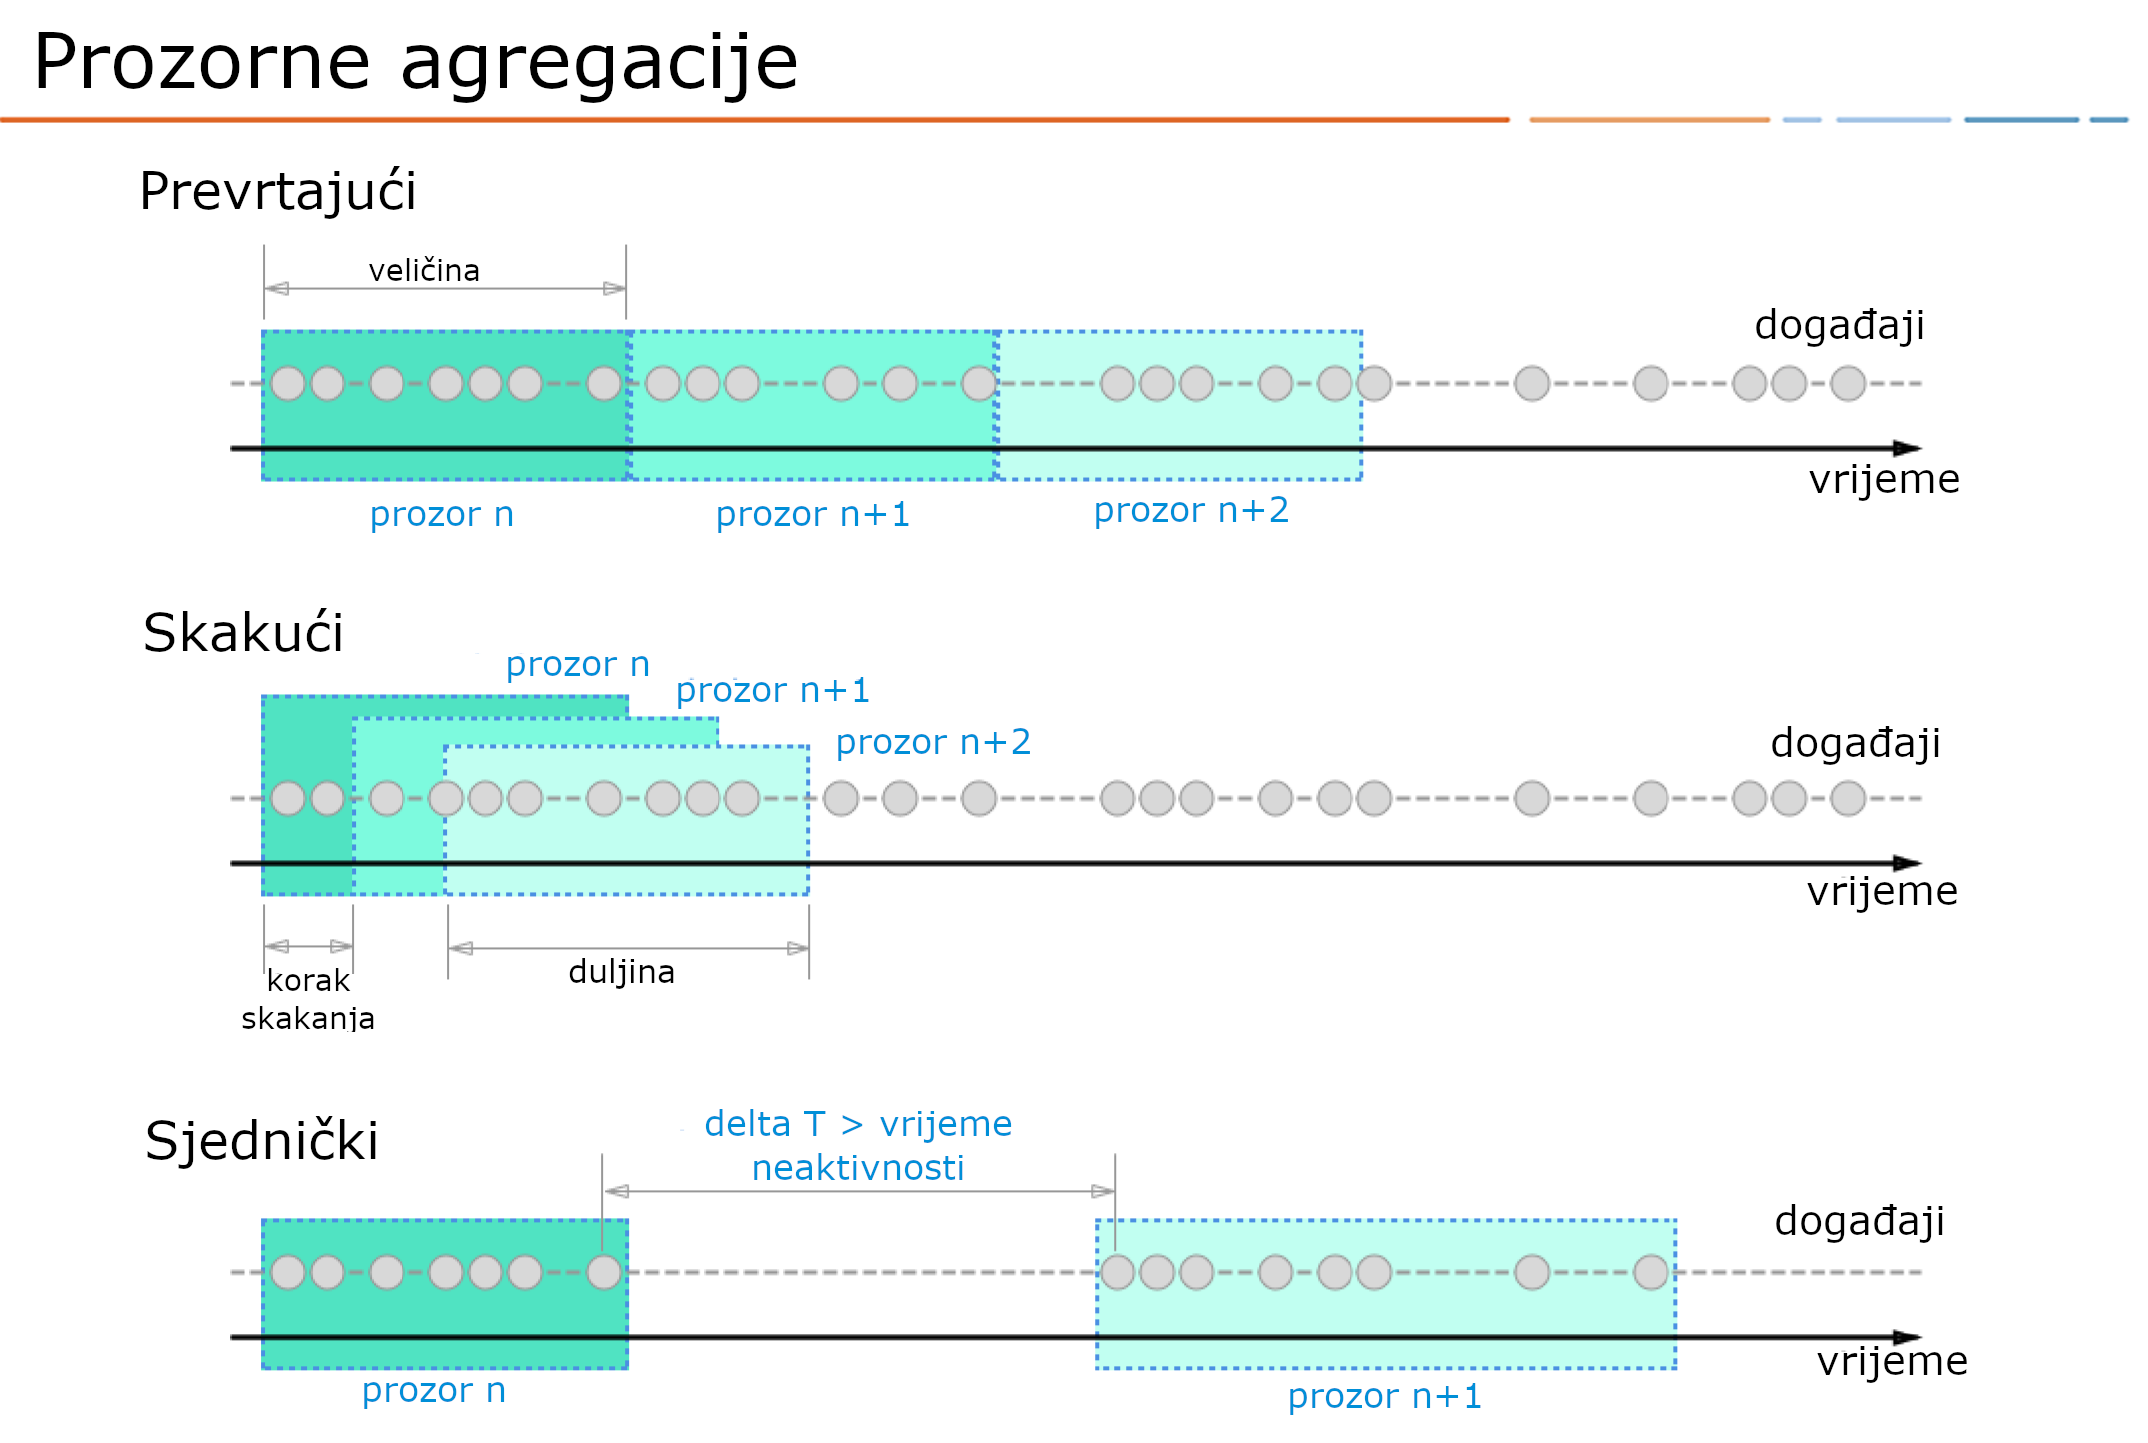
\includegraphics[width=15cm]{images/Windows.png}
	\caption[Prozori agregacija u Kafka Streams-u i ksqlDB-u]{Prozori agregacija u Kafka Streams-u i ksqlDB-u\\Slika preuzeta sa \url{https://docs.ksqldb.io/en/latest/concepts/time-and-windows-in-ksqldb-queries/}}
	\label{fig:windows}
\end{figure}

\subsubsection{Kafka Streams i ksqlDB}

CloudVane se trenutno ne koristi bibliotekom Kafka Streams za obradu tokova podataka, već se oslanja na ksqlDB servis, koji je detaljno opisan u sljedećem poglavlju. No, važno je napomenuti da je ksqlDB zapravo izgrađen na temelju Kafka Streams biblioteke, djelujući kao sloj više razine apstrakcije kao što je prikazano na slici \ref{fig:ksqldb_streams}.

\begin{figure}[htb]
	\centering
	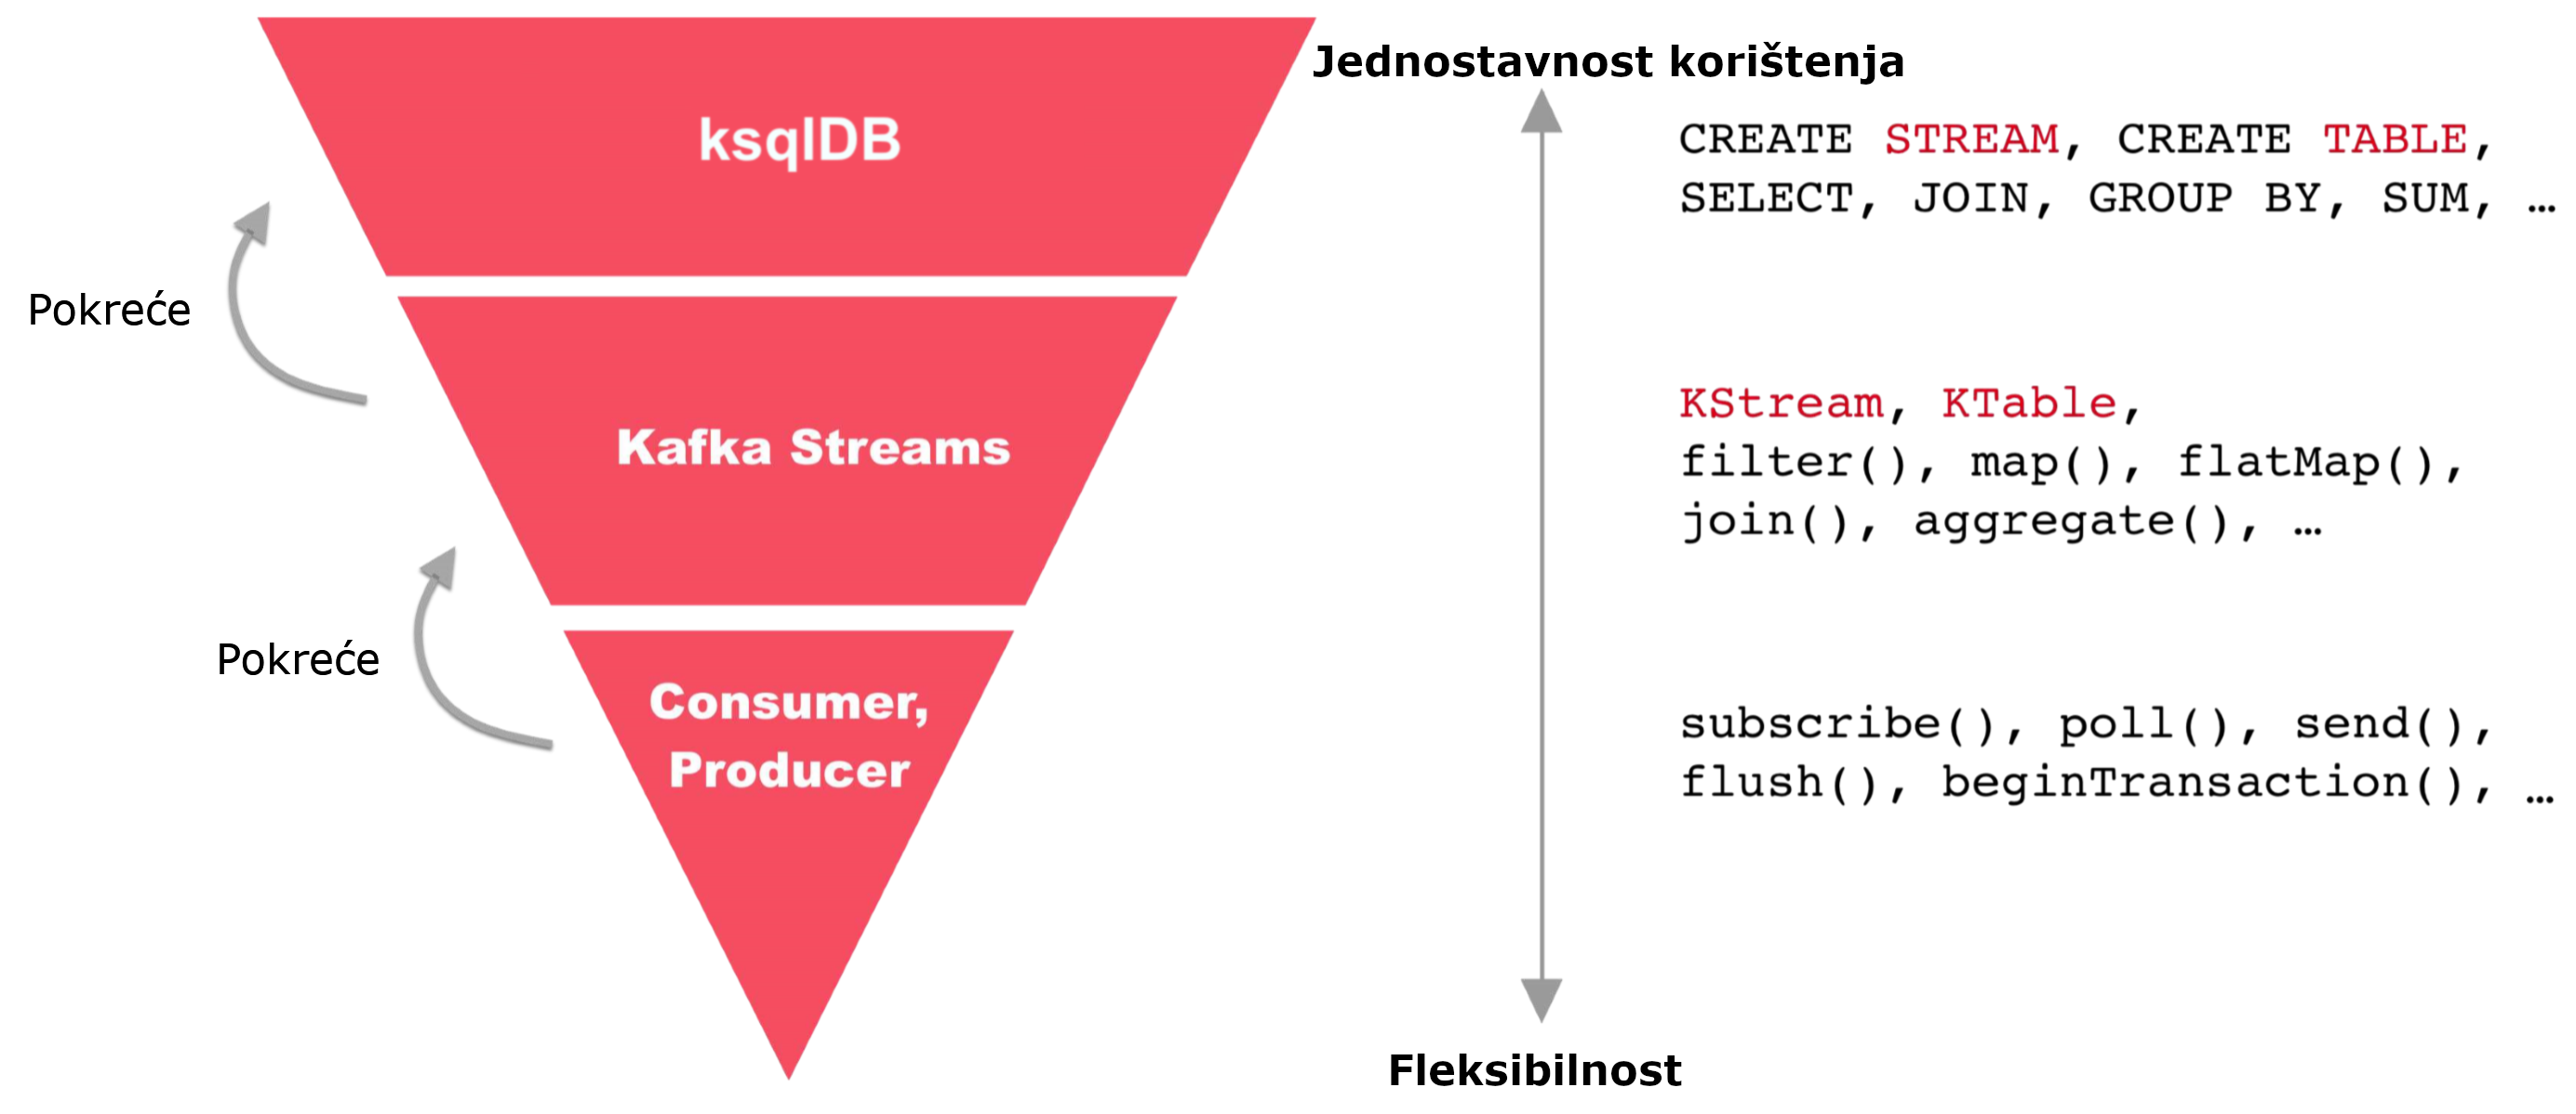
\includegraphics[width=13cm]{images/ksql_streams_consumer.png}
	\caption[Hijerarhija Kafka servisa za obradu tokova podataka]{Hijerarhija Kafka servisa za obradu tokova podataka\\Slika preuzeta sa \url{https://docs.ksqldb.io/en/latest/operate-and-deploy/how-it-works/}}
	\label{fig:ksqldb_streams}
\end{figure}


\subsection{ksqlDB}
\label{sec:ksql}

\textbf{KsqlDB} je specijalizirana baza podataka za obradu tokova događaja \engl{event streaming database}. Ova platforma značajno pojednostavljuje implementaciju, pokretanje i održavanje aplikacija za obradu tokova podataka integrirajući dvije ključne komponente Kafka ekosustava: \emph{Kafka Connect} i \emph{Kafka Streams} \citep{seymour_mastering_2021}.

Kafka Connect, opisan u sljedećem poglavlju, servis je koji omogućuje jednostavno povezivanje Kafke s drugim sustavima. Integracija Kafka Connect-a u ksqlDB omogućuje korisnicima da lako povežu svoje aplikacije s različitim izvorima i odredištima podataka.

Kafka Streams s druge strane, kao što je prikazano na slici \ref{fig:ksqldb_streams}, gradi ksqlDB te omogućuje korisnicima da se koriste funkcionalnostima obrade podataka koje ona pruža, ali s jednostavnošću upita sličnim SQL-u.

KsqlDB, kombinirajući ove dvije komponente, pruža snažnu platformu za obradu tokova podataka. Korisnici mogu jednostavno implementirati složene obrade podataka koristeći jezik sličan poznatom SQL-u, dok ksqlDB obavlja teški posao povezivanja s izvorima i odredištima podataka i obrade podataka u stvarnom vremenu. Ova integracija omogućuje korisnicima da se usredotoče na logiku svojih aplikacija, umjesto na složenosti upravljanja infrastrukturom obrade podataka. \\

CloudVane se oslanja upravo na ksqlDB klaster za obradu, agregaciju i manipulaciju tokova podataka koje prikuplja od podržanih pružatelja oblaka. KsqlDB ne samo da omogućuje agregaciju podataka već i provodi filtriranje i transformaciju podataka, pružajući CloudVane aplikaciji snažan alat za efikasnu i efektivnu obradu podataka.


\subsection{Kafka Connect}
\label{sec:connect}

\textbf{Kafka Connect} je integralni dio Apache Kafka ekosustava i pruža skalabilan te pouzdan način za kopiranje podataka između Kafka i drugih skladišta podataka \citep{shapira_kafka_2021}.

Kafka Connect je dizajniran da podrži veliki broj izvora \engl{source} i odredišta \engl{sink} podataka omogućujući korisnicima da jednostavno povežu Kafku s različitim sustavima za skladištenje podataka. To uključuje tradicionalne baze podataka, datotečne sustave, usluge oblaka i mnoge druge.

Jedna od ključnih funkcionalnosti Kafka Connect-a je njegova sposobnost da se jednostavno horizontalno skalira. To znači da može podržati velike količine podataka i veliki broj veza, što ga čini idealnim za velike, podatkovno intenzivne aplikacije.

Uz to, Kafka Connect podržava neke transformacije podataka omogućujući korisnicima da prilagode podatke kako bi bolje odgovarali njihovim specifičnim potrebama pri ulazu ili izlazu iz Apache Kafke. To može uključivati promjenu formata podataka, dodavanje ili uklanjanje polja, ili nekoliko drugih vrsta manipulacije podacima.

Ukupno gledano, Kafka Connect pruža snažan i fleksibilan način za povezivanje Kafke s različitim skladištima podataka omogućujući korisnicima da maksimalno iskoriste svoje podatke. \\

U kontekstu CloudVane aplikacije Kafka Connect se koristi za prijenos podataka koji su agregirani putem ksqlDB-a u ciljnu bazu podataka, konkretno \emph{Oracle ATP}  bazu.

Ova funkcionalnost omogućava aplikaciji CloudVane da efikasno i pouzdano prenosi obrađene i agregirane podatke iz Kafka ekosustava u \emph{Oracle ATP}, što dalje omogućava naprednu analizu i obradu tih podataka. Korištenje Kafka Connect-a za ovu svrhu osigurava da se podaci prenose na siguran i pouzdan način, uz održavanje visoke razine performansi i mogućnosti skaliranja.

Ova integracija između Kafka Connect-a, ksqlDB-a i Oracle ATP baze podataka omogućava aplikaciji CloudVane da maksimalno iskoristi svoje podatke, pružajući joj snažne alate za obradu podataka u stvarnom vremenu i njihovo pohranjivanje za daljnju analizu i obradu.

\clearpage
\subsection{Avro serializacija i Schema Registry}
\label{sec:schema}

\textbf{Avro} je format serijalizacije podataka neovisan o programskom jeziku što omogućuje njegovu široku primjenu u različitim programskim okruženjima \citep{shapira_kafka_2021}. Glavne prednosti Avro-a su njegova sposobnost smanjenja mrežnog prometa kroz odvajanje sheme podataka od samih vrijednosti i korištenje binarnog formata. Ova značajka omogućuje efikasno upravljanje velikim količinama podataka, što je često ključno u sustavima za obradu podataka u stvarnom vremenu.

Avro također podržava \emph{jaku tipizaciju} \engl{strong typing}, što znači da svaki podatak ima strogo definiran tip. Ova značajka pomaže u sprječavanju pogrešaka i poboljšava pouzdanost obrade podataka jer se mogu izbjeći nekompatibilnosti ili nesporazumi oko formata ili strukture podataka.

Za rad s Apache Kafka sustavom Avro se često koristi u kombinaciji s \textbf{Apache Schema Registry} servisom. Schema Registry je servis koji pomaže u upravljanju shemama i provođenju pravila o shemama osiguravajući da svi podaci koji se upisuju u Kafka teme prate prije definiranu shemu. Ovo je ključno za održavanje kompatibilnosti podataka kako se sustav razvija jer omogućuje promjene u formatu podataka bez gubitka kompatibilnosti s postojećim podacima. \\

Sveukupno, kombinacija Avro-a i Schema Registryja pruža robustan okvir za upravljanje i obradu strukturiranih podataka unutar Apache Kafka sustava. Ove tehnologije omogućuju korisnicima da efikasno i pouzdano upravljaju velikim količinama podataka istovremeno održavajući visoku razinu pouzdanosti i kompatibilnosti. Upravo iz tih razloga CloudVane aplikacija koristi Avro format za pohranu podataka u Kafka teme i Schema Registry servis za održavanje i upravljanje shemama.

Ova praksa omogućuje aplikaciji CloudVane da maksimalno iskoristi prednosti koje Apache Kafka pruža, uključujući skalabilnost, brzinu i pouzdanost. Korištenje Avro formata osigurava da su podaci kompaktni i dobro strukturirani, što poboljšava performanse i omogućuje efikasnu obradu podataka. Istovremeno upotreba Schema Registry servisa osigurava da su sve sheme podataka dosljedno upravljane i održavane, što pomaže u održavanju kvalitete podataka i kompatibilnosti kroz vrijeme.

\subsection{Kafka UI}
\label{sec:kafka-ui}

Pristupanje Apache Kafka sustavu koristeći komandno-linijske alate \engl{Command Line Interface tools} može biti težak i spor proces, pogotovo za korisnike koji nisu iskusni s komandno-linijskim alatima. S druge strane, korištenje grafičkih korisničkih sučelja \engl{Graphical User Interface} pruža nekoliko prednosti koje mogu poboljšati produktivnost i iskustvo rada s Apache Kafka temama, shemama i konektorima.

Korisnička sučelja omogućuju jednostavnije i efikasnije upravljanje jer eliminiraju potrebu za pamćenjem složenih naredbi koje su neophodne za provođenje osnovnih operacija na Apache Kafki. Upravo iz tog razloga, uz Apache Kafka za CloudVane, pokrenut je Kafka UI servis na Kubernetes klasteru.

\section{Arhitektura aplikacije CloudVane}
\label{sec:architecture}

CloudVane, kako je prethodno navedeno, distribuirana je aplikacija koja se izvodi na \emph{Oracle Kubernetes Engine} (OKE) platformi. Osim toga, CloudVane je primjer \emph{mikro-servisne arhitekture}, što znači da se sastoji od brojnih servisa, svaki s određenim zadacima unutar cjelokupnog sustava. Ovi servisi su detaljno opisani u tablici \ref{tbl:cloudvaneServices} i \ref{tbl:kafkaServices}, a cjelokupna arhitektura sustava prikazana je na slici \ref{fig:cloudvaneArch}.\\

Ova struktura omogućuje visoku razinu modularnosti i fleksibilnosti. Svaki servis može se razvijati, skalirati i održavati neovisno o ostalima, što omogućuje brzi razvoj i lako ažuriranje. Također, ova arhitektura omogućuje bolju iskoristivost resursa jer svaki servis može biti skaliran prema svojim specifičnim potrebama.

U kontekstu CloudVane aplikacije, ova mikro-servisna arhitektura omogućuje efikasno upravljanje i obradu velikih količina podataka. Svaki servis može se specijalizirati za određeni aspekt obrade podataka, što rezultira visokom performansom i pouzdanošću cjelokupnog sustava. Detaljan opis svakog CloudVane servisa može se pronaći u tablici \ref{tbl:cloudvaneServices}.

Uzimajući u obzir da CloudVane koristi usluge Apache Kafke, te usluge su smještene u zasebnom Kubernetes prostoru imena u odnosu na glavne servise aplikacije CloudVane. Apache Kafka servisi opisani su u tablici \ref{tbl:kafkaServices}, a protok podataka kroz CloudVane sustav prikazan je na slici \ref{fig:dataCloudvane}.

Ova organizacijska struktura, koja uključuje odvajanje produkcijskog klastera od klastera za razvoj i testiranje, omogućuje jasnu segregaciju i izolaciju resursa među različitim komponentama sustava. Takva struktura ne samo da pojačava sigurnost i upravljivost sustava već i olakšava skaliranje i održavanje svake komponente neovisno jedna o drugoj. Osim toga, ovakva organizacija pruža bolju kontrolu nad resursima te olakšava praćenje i dijagnostiku problema unutar sustava. U konačnici, ovakav pristup omogućuje efikasnije upravljanje resursima i optimizaciju performansi, čime se poboljšava ukupna pouzdanost i efikasnost CloudVane aplikacije.

\clearpage
\begin{longtblr}[
  	caption = {CloudVane servisi na Kubernetesu},
	label = {tbl:cloudvaneServices},
	]{
	colspec = {X[1,l]|X[1,c]}, 
	rowhead = 1,
	}
	\hline
	Naziv servisa & Opis servisa \\
	\hline
	CloudVane Actioner & Upravlja akcijama na oblaku\\
	CloudVane API & REST poslužitelj i autentifikacija\\
	CloudVane Back & Spring poslužiteljske strane\\
	CloudVane Chargeback & Omogućuje izradu izvještaja o potrošnji\\
	CloudVane Config & Spring Config server\\
	CloudVane Datacollector Kafka & Dohvaća podatke iz oblaka, obrađuje ih i prosljeđuje u Apache Kafku\\
	CloudVane Datacollector & Dohvaća podatke iz oblaka, obrađuje ih i pohranjuje direktno u bazu podataka\\
	CloudVane Front & Angular poslužitelj klijentske strane \\
	CloudVane Predictioner API & REST poslužitelj predikcijskog sustava\\
	CloudVane Predictioner Worker & Sustav umjetne inteligencije koji računa predikcije\\
	CloudVane Scheduler & Raspoređivač zadataka CloudVane aplikacije\\
	CloudVane User Management & Sustav za upravljanje korisnicima i autorizaciju \\
	CloudVane Vault & Sustav za sigurnu pohranu korisničkih kredencijala \\
	\hline

\end{longtblr}

\begin{longtblr}[
	caption = {Kafka servisi na CloudVane Kubernetesu},
	label = {tbl:kafkaServices},
	]{
		colspec = {X[1,l]|X[1,c]}, 
		rowhead = 1,
	}
	\hline
	Naziv Kafka servisa & Opis servisa \\
	\hline
	Kafka Broker & Poslužuje Apache Kafku\\
	Kafka Connect klaster & Upis tokova u bazu podataka\\
	ksqlDB & Obrađuje tokove podataka\\
	Schema Registry & Upravlja shemama podataka\\
	Kafka UI & Jednostavan pregled Kafka tema
	\hline
	
\end{longtblr}


\section{CloudVane kao izvor podataka}

U okviru ovog rada svi će dnevnički zapisi prethodno opisanih servisa biti preusmjereni iz testne okoline CloudVane klastera u Kafka teme, koje se nalaze u Apache Kafki na lokalnom Kubernetes klasteru. Takva struktura omogućit će efikasnu obradu zapisa te njihovo korištenje za generiranje rezultata istraživanja.

Metodologija i alati potrebni za praćenje aplikacije CloudVane bit će opisani u sljedećim poglavljima. Ovim pristupom osigurava se jasan i detaljan uvid u kompleksni proces obrade podataka u stvarnom vremenu koristeći kombinaciju Apache Kafka, Kubernetes i drugih alata te tehnologija.

\chapter{Nadziranje aplikacija}
\label{sec:monitoring}

\textbf{Nadziranje} \engl{monitoring}, definirano kao sustavno promatranje i provjera ponašanja i izlaza sustava te njegovih komponenti kroz vrijeme \citep{monitorama_monitorama_2016}, ključni je element upravljanja informatičkim sustavima i aplikacijama. Ova strateška praksa, koja se sastoji od stalnog nadzora i analize, omogućuje održavanje optimalnih performansi, stabilnosti i pouzdanosti digitalnih resursa.

Nadzor aplikacija nije samo proces identifikacije i rješavanja problema. On nudi dragocjene uvide koji omogućuju temeljitiju optimizaciju sustava, poboljšanje korisničkog iskustva i osiguranje da se sve digitalne komponente funkcionalno integriraju. Sastoji se od kontinuirane provjere, identifikacije anomalija i promptnog rješavanja problema prije nego što se pretvore u kritične situacije. Ovim proaktivnim pristupom nadzor postaje ključan instrument za održavanje visoke razine usluge i postizanje operativne izvrsnosti.\\

U ovom poglavlju rada detaljno se istražuje nadzor aplikacija poput aplikacije CloudVane, koja je opisana u poglavlju \ref{sec:cloudvane}, s posebnim naglaskom na kontekst \emph{dnevničkih zapisa} prikazanih u poglavlju \ref{sec:logs} iz \emph{distribuiranih mikro-servisnih sustava}. Upotrebom alata \emph{ELK}, čije su komponente i funkcionalnosti predstavljene u poglavlju \ref{sec:elk}, ilustrirat će se korištenje sofisticiranih alata za izdvajanje dnevničkih zapisa iz distribuiranih aplikacija unutar Kubernetes grozda. Detaljno će se obraditi procesi prikaza, transformacije i unosa dnevničkih zapisa u Apache Kafku.

\clearpage
\section{Dnevnički zapisi}
\label{sec:logs}

\textbf{Dnevnički zapisi} aplikacija \engl{application logs} ključna su komponenta koja pruža detaljan uvid u rad aplikacije te su ključni za otkrivanje i rješavanje problema, ali i za optimizaciju performansi aplikacije.\\

Dnevnički zapisi aplikacija sastoje se od sekvencijalno zapisanih događaja koji se generiraju unutar aplikacije. Ti događaji mogu biti različite vrste, uključujući informacije o radnji koju je korisnik poduzeo, statusu aplikacije, greškama, upozorenjima i drugim relevantnim informacijama. Dnevnički zapisi pružaju sveobuhvatnu sliku o tome što se događa unutar aplikacije u svakom trenutku.\\

U kontekstu \emph{mikro-servisnih arhitektura}, kao što je to slučaj s CloudVane aplikacijom, dnevnički su zapisi posebno važni. Budući da je svaki mikro-servis odgovoran za svoj dio funkcionalnosti, dnevnički zapisi svakog mikro-servisa pružaju uvid u rad cijele aplikacije. Ako dođe do problema, dnevnički zapisi mogu pomoći u identificiranju komponente koja je uzrokovala problem.

Međutim, upravljanje dnevničkim zapisima u mikro-servisnom okruženju može biti izazovno. Jedan od najizraženijih problema jest problem agregiranja i pretraživanja dnevničkih zapisa. S obzirom na to da je aplikacija raspoređena na više čvorova unutar Kubernetes grozda koji su izolirani, konsolidacija i pretraživanje informacija postaje kompleksan zadatak \citep{newman_building_2015}.

U takvom distribuiranom okruženju, svaka komponenta ili mikro-servis generira svoje dnevničke zapise. S obzirom na to da su ovi dnevnički zapisi disperzirani preko različitih čvorova, njihova centralizacija zahtijeva robusna i skalabilna rješenja. Bez odgovarajućih alata i strategija pretraživanje tih zapisa na jednom mjestu može biti prilično izazovno i vremenski zahtjevno. Osim toga, pitanje je i kako oblikovati i strukturirati te zapise tako da pružaju korisne informacije. Različiti mikro-servisi mogu imati različite strukture dnevničkih zapisa. Zahtijeva se strategija koja ne samo da agregira ove zapise već ih i standardizira i strukturira za laku analizu i dijagnostiku. \\

U nastavku poglavlja fokus će se staviti na dnevničke zapise programskog jezika \emph{Java}. Fokus na programski jezik Javu proizlazi iz činjenice da je većina servisa unutar distribuirane aplikacije CloudVane razvijena upravo ovim programskim jezikom. Iako i drugi programski jezici nude slične alate za konfiguraciju i upravljanje dnevničkim zapisima, specifičnosti Jave u ovom kontekstu su od posebne važnosti zbog potrebnih konfiguracija. Također, posvetit će se pažnja ELK alatima, što je centralna tema poglavlja \ref{sec:elk}. Ova dva aspekta čine ključne komponente istraživanja i analize nadzora aplikacija unutar distribuiranih sustava.


\subsection{Dnevnički zapisi u programskom jeziku Java}
\label{sec:java}

CloudVane koristi \textbf{Logback biblioteku} za svoje potrebe generiranja dnevničkih zapisa, također koristeći \textbf{SLF4J apstrakciju}\footnote{SLF4J nudi mogućnost generičkog pisanja dnevničkih zapisa u programskom kodu neovisno o konkretnoj implementaciji sustava generiranja dnevničkih zapisa.} koju nudi biblioteka \emph{Spring}. Logback je konfiguriran da ispisuje dnevničke zapise u JSON formatu, što olakšava njihovu obradu, posebno u distribuiranom sustavu gdje različiti servisi generiraju zapise. Primjer konfiguracije Logback-a na aplikaciji CloudVane prikazan je u isječku \ref{lst:logback_xml}.

Primjer jednog dnevničkog zapisa prikazan je u isječku \ref{lst:cloudvaneLog}. Ovaj zapis ilustrira kako se informacije strukturiraju u JSON formatu.\\

Osim \emph{Logback}, postoji i \emph{Log4j} biblioteka, koja je također popularna opcija za dnevničke zapise u Java aplikacijama. Međutim, u kontekstu CloudVane aplikacije, Logback je odabran zbog fleksibilnosti u konfiguraciji.


\section{Elastic, Logstash i Kibana (ELK)}
\label{sec:elk}

\textbf{ELK}, akronim koji označava \textbf{ElasticSearch}, \textbf{Logstash} i \textbf{Kibana}, predstavlja snažan skup alata sposoban za prikupljanje, pohranu, analizu i vizualizaciju podataka u stvarnom vremenu. Najčešće se koristi za upravljanje dnevničkim zapisima i praćenje događaja, što ga čini nezamjenjivim alatom za sigurnosne analize, poslovnu inteligenciju i efikasno pretraživanje podataka.

U ovom se poglavlju detaljno razmatraju funkcionalnosti svake pojedinačne komponente ELK-a te se opisuje njegova uloga u rješenju koje predlaže ovaj rad.

\subsection{ElasticSearch}
\label{sec:elastic}

\textbf{Elasticsearch} je distribuirani sustav za pretragu i analizu podataka u stvarnom vremenu. Omogućava istraživanje podataka na brz i skalabilan način koji do sada nije bio ostvariv. Koristi se za pretragu cijelog teksta, strukturiranu pretragu, analitiku i kombinaciju svih triju funkcionalnosti \citep{gormley_elasticsearch_2015}.

Zasnovan na \emph{Apache Lucene-u}\footnote{Apache Lucene je snažan sustav za pretraživanje teksta otvorenog koda koji se koristi u brojnim aplikacijama za pretragu i analizu podataka.}, Elasticsearch pruža distribuirani sustav za pretragu teksta s HTTP sučeljem. Ovo sučelje omogućuje jednostavan pristup i manipulaciju podacima kroz standardizirane HTTP protokole. \\

U okviru ELK-a, Elasticsearch igra ključnu ulogu kao središnje mjesto za pohranu svih podataka. U kontekstu ovoga rada, to su dnevnički zapisi prikupljeni pomoću Logstash-a, komponente zadužene za njihovo prikupljanje, transformaciju i slanje u Elasticsearch, opisane u poglavlju \ref{sec:logstash}.\\

Elasticsearch ne samo da omogućava pohranu podataka već nudi i mogućnosti za njihovu detaljnu analizu i pretragu. Ove mogućnosti, u kombinaciji sa skalabilnošću i brzinom koju pruža, čine Elasticsearch idealnim izborom za upravljanje velikim količinama podataka u stvarnom vremenu \engl{real-time}.

\subsubsection{Indeksi u ElasticSearch-u}

Indeks u kontekstu ElasticSearch-a je osnovna jedinica za pretragu. Predstavlja kolekciju dokumenata koji imaju slične karakteristike. Indeks je identificiran svojim jedinstvenim imenom, koje se koristi prilikom izvršavanja operacija pretrage, ažuriranja, brisanja i indeksiranja na dokumentima. U ovom se radu indeks koristi za organiziranje i skladištenje dnevničkih zapisa omogućavajući njihovu brzu i efikasnu pretragu.

\subsection{Logstash}
\label{sec:logstash}

\textbf{Logstash} je servis otvorenog koda i predstavlja snažan sustav za obradu podataka. Njegova je glavna svrha izvlačenje podataka iz različitih izvora, njihova transformacija i obogaćivanje te naknadno slanje prema odredištu \citep{konda_elasticsearch_2023}. Zahvaljujući arhitekturi koja je bazirana na obradi tokova podataka, svaki događaj koji prođe kroz Logstash obrađuje se sukladno prethodno konfiguriranim pravilima i u stvarnom vremenu se prosljeđuje na odredište. To omogućava kontinuiranu obradu podataka, što je posebno primjenjivo u kritičnim sustavima, kao što su oni koji se bave analizom grešaka izvučenih iz dnevničkih zapisa.\\

U okviru ovog rada Logstash igra ključnu ulogu prikupljajući dnevničke zapise iz različitih Apache Kafka tema. Zatim se zapisi upisuju u ElasticSearch indeks, nakon čega se mogu pretraživati i postaju lako dostupni za daljnju analizu.

\subsection{Kibana}
\label{sec:kibana}

\citet{gormley_elasticsearch_2015} navode da je \textbf{Kibana} višenamjenska konzola koja nudi niz opcija, od izvršavanja upita do razvoja nadzornih ploča, grafova i vizualizacija dijagrama za detaljnu analizu i agregacije. Međutim, za komunikaciju s ElasticSearch-om i pozivanje API-ja nije nužno koristiti Kibanu. Na primjer, API-je ElasticSearch-a možemo pozivati koristeći \emph{cURL}, \emph{Postman} ili klijente nekog programskog jezika.\\

Kibana, kao alat za vizualizaciju i istraživanje podataka, u ovom radu koristi se kao sučelje na kojem se mogu kreirati intuitivni grafikoni i izvješća. Ovi elementi omogućuju interaktivno navigiranje kroz velike količine dnevničkih zapisa. S Kibanom je moguće konfigurirati nadzorne ploče koje pružaju vizualne sažetke podataka i omogućuju detaljno istraživanje specifičnih događaja. Primjer prikaza alata Kibane s dnevničkim zapisima može se vidjeti na slici \ref{fig:kibana}.\\

Kibana pruža mogućnost vizualizacije podataka pohranjenih u ElasticSearch-u koristeći njene snažne mogućnosti upita i filtriranja. Time se omogućuje detaljna analiza specifičnih metrika ili trendova. Ova funkcionalnost je ključna za učinkovito analiziranje i razumijevanje obimnih podatkovnih setova, kao što su dnevnički zapisi koje obrađuje ovaj rad.

\begin{figure}[htb]
	\centering
	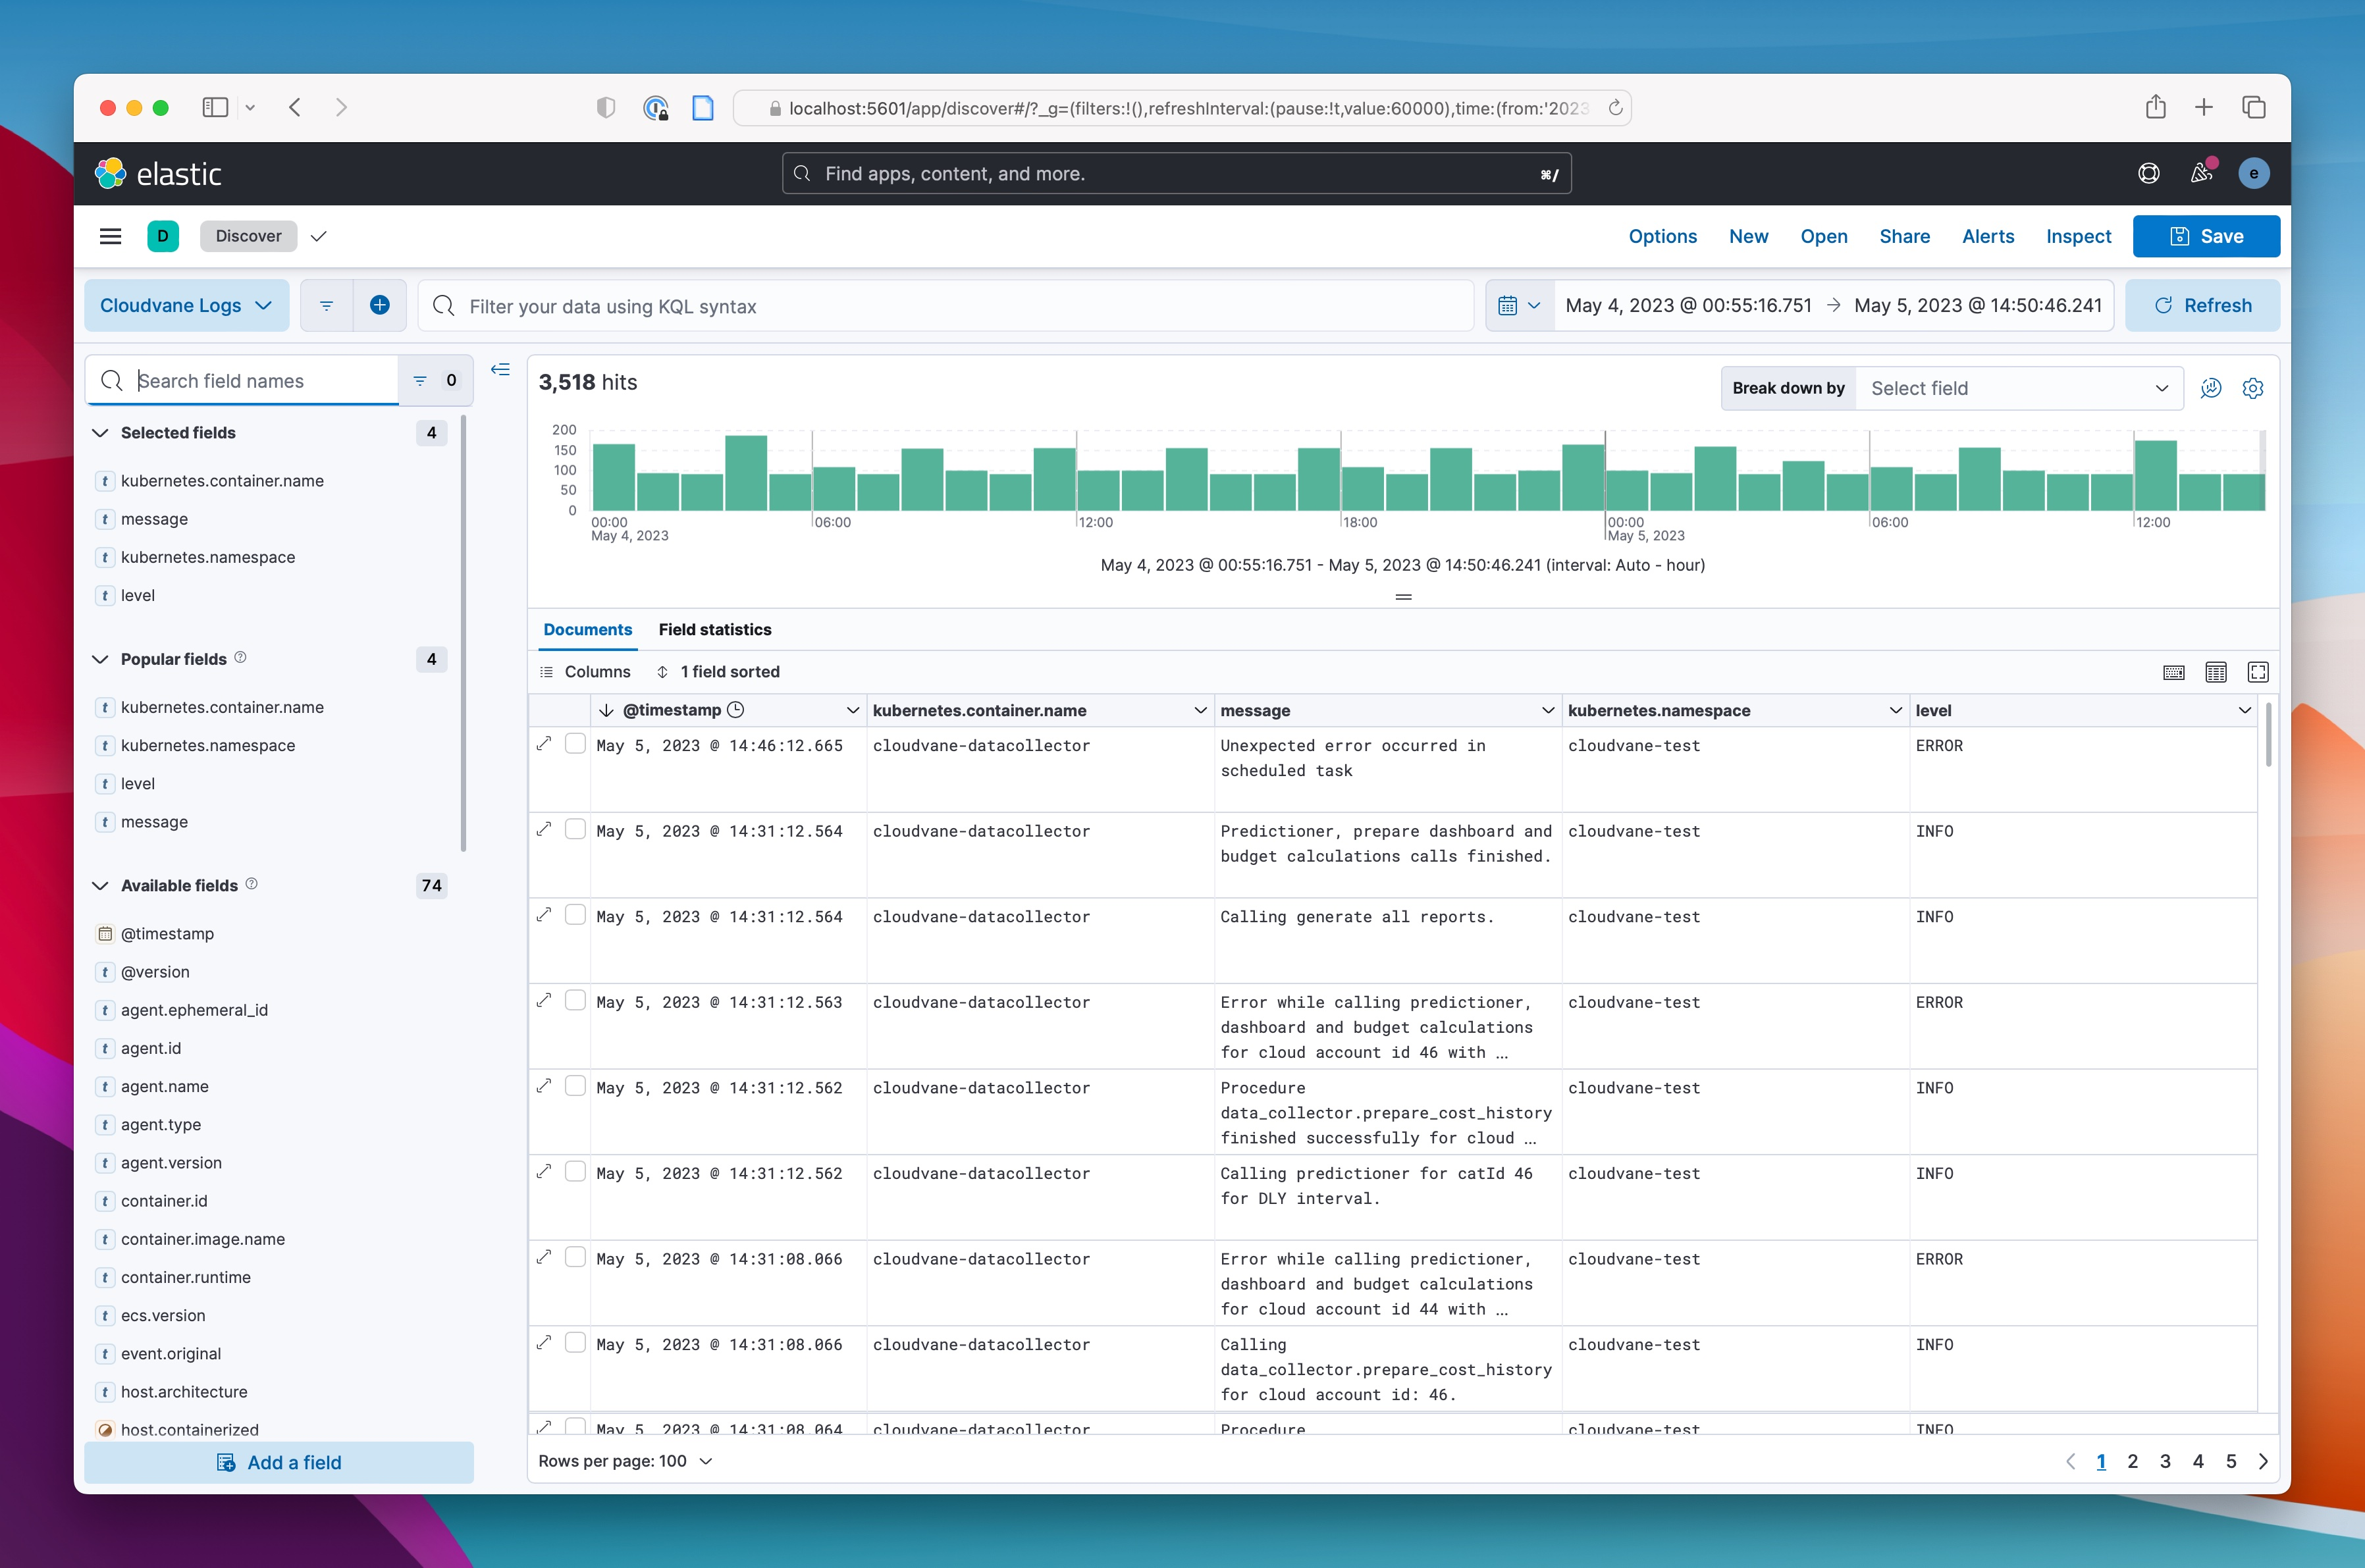
\includegraphics[width=15cm]{images/elastic-logs.jpeg}
	\caption[Kibana sučelje]{Kibana sučelje}
	\label{fig:kibana}
\end{figure}

\subsection{Filebeat}
\label{sec:filebeat}

\textbf{Filebeat} je alat za prikupljanje podataka čiji je glavni zadatak skupljanje i centralizacija dnevničkih zapisa. Njegova je uloga u ELK-u nadziranje specifične datoteke s dnevničkim zapisima, njihovo prikupljanje i zatim prosljeđivanje izravno u ElasticSearch indeks ili u Logstash za daljnju obradu. 

Filebeat je samo jedan od mnogih alata u sklopu Beats platforme koju je razvila tvrtka Elastic. Beats je platforma koja se sastoji od niza alata za prikupljanje podataka, uključujući dnevničke zapise, mrežni promet, metrike i slično. Svi alati unutar Beats platforme razvijeni su s ciljem jednostavnosti i učinkovitosti. 

Zbog svog dizajna koji naglašava jednostavnost i minimalnu potrošnju resursa, Filebeat je iznimno pogodan za distribuirane okoline poput Kubernetesa.\\

Iako Logstash nudi značajne mogućnosti obrade podataka, Filebeat je specijaliziran da bude lagan i brz, s naglaskom na efikasno prikupljanje dnevničkih zapisa i njihovo brzo prosljeđivanje do odredišta. To znači da se Filebeat može pokrenuti, a da se to ne odrazi značajno na performanse. Filebeat i Logstash često se koriste u tandemu; \emph{Filebeat} je odgovoran za prikupljanje i prosljeđivanje dnevničkih zapisa, a \emph{Logstash} ih zatim obrađuje i obogaćuje prije konačnog indeksiranja u ElasticSearch-u.\\

U okviru ovog rada, Filebeat je pokrenut na CloudVane Kubernetes klasteru u obliku Kubernetes DaemonSet-a te je konfiguriran da prikuplja dnevničke zapise s CloudVane servisa na testnoj okolini. Nakon prikupljanja ti se dnevnički zapisi prosljeđuju preko interneta na lokalni Minikube Kubernetes klaster, točnije u Apache Kafka teme što je detaljnije opisano u poglavlju \ref{sec:kafkaImpl}. 

S obzirom na to da se Filebeat pokreće na Kubernetesu kao DaemonSet, pokreće se u onoliko instanci koliko čvorova ima grozd. Jedna instanca Filebeat-a po čvoru omogućuje Filebeat-u pristup kontejnerima koji se na njemu vrte. Konfiguracija ovoga servisa implementirana je kao Kubernetes ConfigMap i pokazana je u isječku koda \ref{lst:filebeat}.

\subsection{Implementacija ELK-a na Kubernetes grozdu}
\label{sec:elk_impl}

U ovom radu su ElasticSearch, Kibana i Logstash implementirani u lokalnom Kubernetes klasteru koristeći ELK CRD-ove. Elastic, kompanija koja stoji iza razvoja ovih aplikacija, kreirala je CRD-ove za te programe kako bi se olakšala njihova implementacija na Kubernetes klasteru. To omogućava korisnicima da jednostavno postave aplikacije i upravljaju tim aplikacijama unutar Kubernetes okruženja pružajući im integrirane mogućnosti za konfiguraciju, skaliranje, sigurnost i nadzor.\\

Filebeat je međutim, kao što je prethodno opisano, pokrenut na CloudVane Kubernetes grozdu kao DaemonSet, a njegova konfiguracija je pružena putem ConfigMap objekta.

\chapter{Nadziranje stanja distribuiranog sustava u stvarnom vremenu}
\label{sec:streamingMonitoring}

Kao što je prethodno spomenuto u poglavlju \ref{sec:monitoring}, nadziranje aplikacija ključno je za održavanje optimalnih performansi, stabilnosti i pouzdanosti aplikacija. Strukturirano i sustavno nadziranje može biti presudno za otkrivanje i rješavanje problema prije nego što oni počnu utjecati na korisnike ili poslovanje.

Dok su suvremene aplikacije postale sve složenije, zadatak njihova nadzora postao je izrazito zahtjevan. Ovaj je izazov posebno istaknut kod nadziranja distribuiranih sustava, gdje svaki individualni servis može potencijalno postati točka slabosti ili čak izazvati potpuni sistemski neuspjeh.

S takvom razinom kompleksnosti nadziranje distribuiranih sustava prelazi granice jednostavnog praćenja pojedinačnih servisa i zahtijeva upotrebu sveobuhvatnih alata za nadzor. Nadzor nije samo otkrivanje grešaka ili slabosti unutar pojedinačnih servisa. Osim toga, nužno je uspostaviti sistemski pregled, identificirati anomalije u stvarnom vremenu, reagirati pravodobno i učinkovito kako bi se osigurao nesmetan rad distribuiranih sustava.

U tom je kontekstu potrebno koristiti napredne alate za nadzor koji omogućuju dubinsko praćenje performansi i stanja svih servisa, bez obzira na to gdje se nalaze. Ti alati trebaju omogućiti brzo otkrivanje problema, detaljne informacije o prirodi problema i omogućiti promptno djelovanje kako bi se osigurali optimalan rad i performanse distribuiranih sustava. Ovakav pristup osigurava visoku razinu pouzdanosti i stabilnosti omogućujući sustavima da stalo pružaju visokokvalitetnu uslugu korisnicima.\\

U nadolazećim poglavljima rada obrađuje se arhitektura rješenja koja omogućava agregiranje dnevničkih zapisa svih servisa distribuirane aplikacije CloudVane u stvarnom vremenu. Ovo rješenje ne samo da filtrira zapise prema njihovom statusu već koristi i umjetnu inteligenciju kako bi prepoznalo potencijalne probleme i ponudilo moguća rješenja.

Zatim se problem, zajedno s predloženim rješenjima, korisniku prezentira kroz sustav notifikacija. Osim toga, rješenje uključuje vizualizaciju svih relevantnih podataka unutar Kibane, što korisnicima omogućava brzo i intuitivno razumijevanje stanja njihove aplikacije. Ovo sveobuhvatno rješenje omogućuje korisnicima da brzo reagiraju na potencijalne probleme, čime se unapređuje ukupna stabilnost i performanse distribuiranih aplikacija.

\section{Pregled arhitekture rješenja}

Kako je već spomenuto u prethodnim poglavljima, arhitektura rješenja, koje je predmet ovog rada, vidljiva na slici \ref{fig:archDiagram}, sastoji se od više komponenata koje zajedno formiraju sveobuhvatni sustav za nadzor distribuiranih aplikacija. Ovaj sustav, koji je implementiran na lokalnom Minikube Kubernetes grozdu te djelomično na CloudVane Kubernetes grozdu, omogućuje kontinuirano praćenje, analizu i rješavanje problema unutar aplikacija.\\

\begin{figure}[htb]
	\centering
	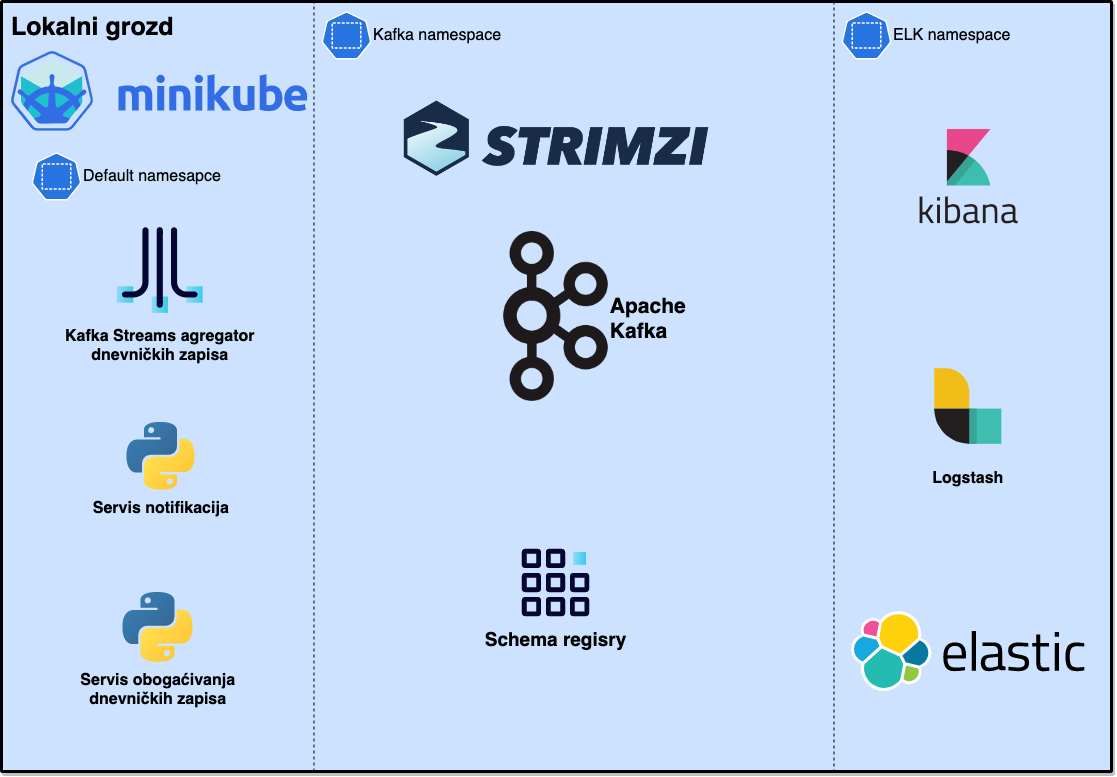
\includegraphics[width=15cm]{images/ThesisArchitecture.png}
	\caption[Arhitektura sustava]{Arhitektura sustava}
	\label{fig:archDiagram}
\end{figure}

Na CloudVane Kubernetes grozdu je pokrenut \textbf{Filebeat servis} koji je odgovoran za prikupljanje dnevnika svih servisa aplikacije. Kako je opisano u poglavlju \ref{sec:filebeat}, Filebeat dnevničke zapise zatim šalje preko interneta na teme Apache Kafke koja je pokrenuta u lokalnom Minikube grozdu. Budući da se ovi podaci prenose preko interneta, Apache Kafka je zaštićena TLS-om\footnote{TLS (Transport Layer Security) je protokol koji osigurava zaštitu podataka tijekom prijenosa preko interneta.} kako bi se osigurao siguran prijenos podataka. Na slici \ref{fig:dataDiagram} vidljiv je protok dnevničkih zapisa kroz sustav.

\begin{figure}[htb]
	\centering
	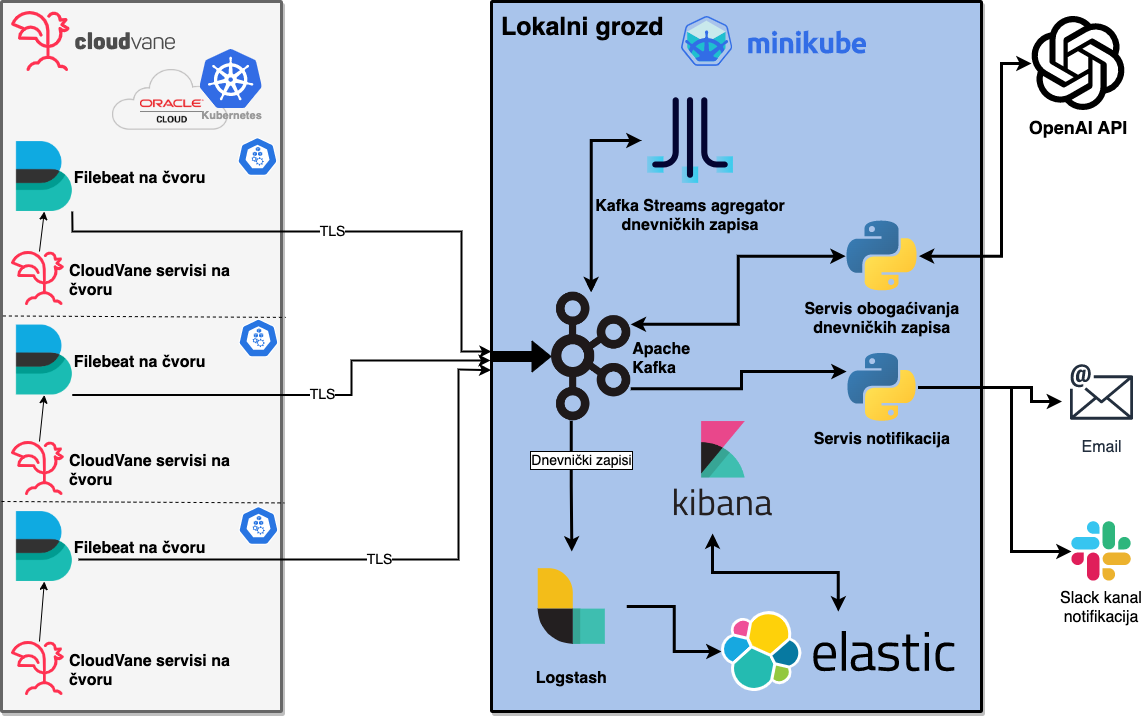
\includegraphics[width=15cm]{images/ThesisData.png}
	\caption[Tok podataka sustava]{Tok podataka \engl{data pipeline} sustava}
	\label{fig:dataDiagram}
\end{figure}

Na lokalnom Kubernetes Minikube grozdu pokrenuta je \textbf{Apache Kafka} pomoću alata \textbf{Strimzi}. Uz jedan Apache Kafka posrednik\footnote{S obzirom na to da se Minikube sastoji samo od jednoga čvora, nema razloga pokretati više replika posrednika \engl{brokera}.} \engl{broker} pokrenut preko alata Strimzi, pokrenut je i Schema Registry servis za upravljanje shemama podataka. U poglavlju \ref{sec:kafkaImpl} opisani su implementacijski detalji lokalne instance Apache Kafke i Kafka teme koje se koriste za pohranu dnevničkih zapisa.

Nakon Apache Kafke na lokalnom je Kubernetes grozdu pokrenuta i distribuirana \textbf{Kafka Streams aplikacija} koja filtrira i agregira dnevničke zapise. Ova aplikacija je detaljno opisana u poglavlju \ref{sec:streamImpl}. Agregirani dnevnički zapisi zatim se šalju natrag u nove, agregirane Kafka teme, a taj je protok vidljiv na dijagramu \ref{fig:topics}.

\begin{figure}[htb]
	\centering
	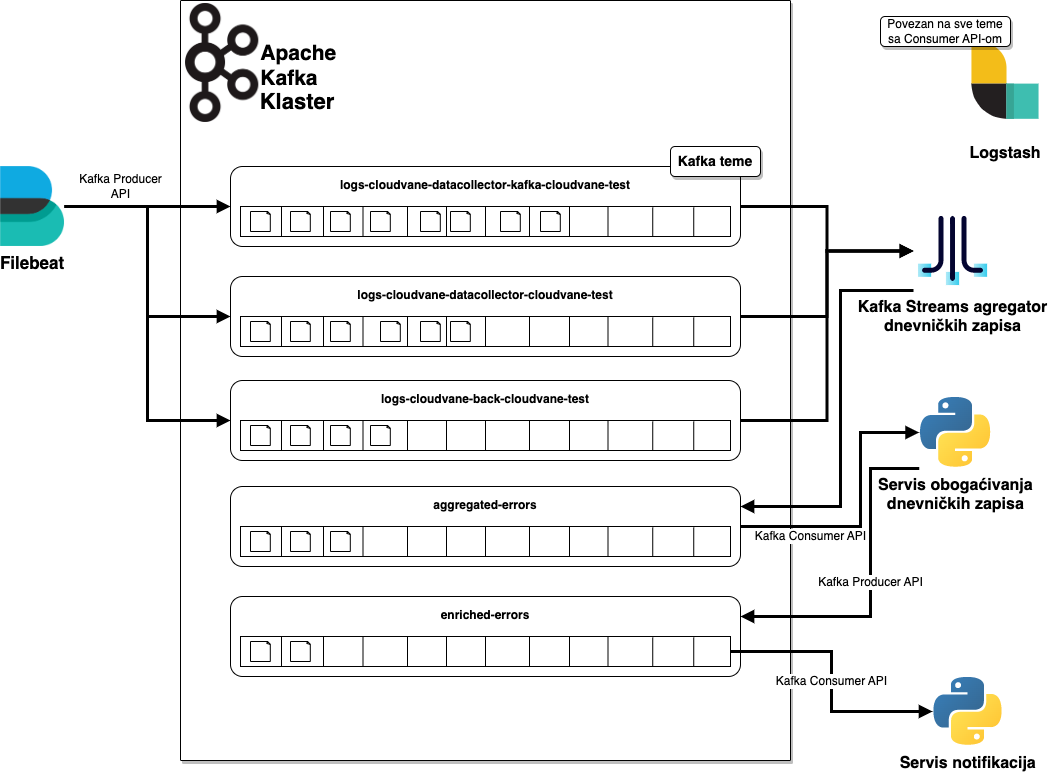
\includegraphics[width=15cm]{images/KafkaTopics.png}
	\caption[Kafka teme s dnevničkim zapisima]{Kafka teme \engl{topics} s dnevničkim zapisima \engl{logs}}
	\label{fig:topics}
\end{figure}

Paralelno s tim, \textbf{servis za obogaćivanje dnevničkih zapisa} pokrenut je na Kubernetes grozdu i opisan je u poglavlju \ref{sec:ai}. Ovaj servis je dizajniran da bude skalabilan i prilagodljiv, ovisno o potrebama sustava. Za svaku grešku koja se javlja u CloudVane aplikaciji i koja se detektira u dnevničkom zapisu, ovaj servis komunicira s API-jem usluge umjetne inteligencije kako bi pronašao potencijalno rješenje. Svaka detektirana greška, zajedno sa sugeriranim rješenjem, zatim se šalje u novu Kafka temu kao što je vidljivo u dijagramu \ref{fig:topics}.

Na sve teme koje sadrže dnevničke zapise spojen je \textbf{Logstash servis}, opisan u poglavlju \ref{sec:logstash} i prikazan u dijagramu \ref{fig:dataDiagram}. Logstash skuplja dnevničke zapise iz svih tema, a zatim ih prosljeđuje u \textbf{ElasticSearch} indekse. Ova funkcionalnost omogućuje korisnicima da putem \textbf{Kibane} iz poglavlja \ref{sec:kibana}, imaju cjelovit uvid u dnevničke zapise, bilo da su agregirani ili ne. Implementacija pregleda dnevničkih zapisa kroz Kibanu demonstrirana je u poglavlju \ref{sec:kibanaImpl}.

Konačno, kako bi korisnici bili u stvarnom vremenu informirani o svim greškama koje se javljaju u aplikaciji, implementiran je i \textbf{servis za notifikacije}. Ovaj servis, opisan u poglavlju \ref{sec:notifService} i vizualiziran u dijagramu \ref{fig:dataDiagram}, obavještava korisnike o svim detektiranim problemima putem različitih kanala komunikacije uključujući elektroničku poštu, mobilne notifikacije i Slack kanal.\\

Ova visoko integrirana arhitektura omogućuje proaktivni pristup upravljanju distribuiranim aplikacijama, omogućujući korisnicima da brzo reagiraju na probleme i osiguraju maksimalnu učinkovitost i pouzdanost svojih aplikacija.


\section{Kubernetes infrastruktura rješenja}
\label{sec:localKubernetes}

Kao što je prethodno istaknuto, i prema dijagramu \ref{fig:archDiagram}, sve komponente ovog rješenja implementirane su na lokalnom Kubernetes Minikube klasteru. Jedini izuzetak je Filebeat servis, koji je pokrenut na CloudVane Kubernetes klasteru, što je detaljnije objašnjeno u poglavlju \ref{sec:filebeat}.\\

Na Kubernetes klasteru stvorena su dva dodatna prostora imena \engl{Namespace}. Prvi, pod imenom \emph{\glqq kafka\grqq}, sadrži Kafka servise Strimzi operatora, Schema Registry, Kafka UI te prateće Service objekte za mrežnu komunikaciju s Kafkom. Drugi, imenovan \emph{\glqq elk\grqq}, sadrži ELK servise, uključujući Logstash, Kibanu i ElasticSearch. U \emph{zadanom} \engl{default} prostoru imena nalazi se Kafka Streams aplikacija, uz koju je pokrenut i servis za obogaćivanje i servis za notifikacije.

Sve usluge koje su pokrenute na Minikube klasteru konfigurirane su s jednom replikom, s obzirom na to da se Minikube klaster sastoji od jednog čvora, kao što je navedeno u poglavlju \ref{sec:minikube}. U produkcijskom okruženju broj replika može se povećati jednostavnim izmjenama parametara u konfiguraciji Kubernetes objekata.\\

Za potrebe pristupa Apache Kafka posredniku s interneta, bilo je nužno konfigurirati Strimzi Kafka objekt i omogućiti pristup preko TLS-a. Dodatno, bilo je potrebno kreirati Kafka User objekt na temelju kojeg Strimzi generira kredencijale za autentifikaciju u obliku Secreta. Ti se kredencijali zatim izvlače i kao novi Secret pohranjuju u CloudVane Kubernetes klaster omogućavajući Filebeat servisu slanje dnevničkih zapisa u Minikube klaster.\\

ELK alati, uključujući ElasticSearch, Filebeat i Kibanu, također generiraju kredencijale za pristup u obliku Secret objekta. Iz Secret objekta je potrebno izvući te podatke kako bi se omogućila autentifikacija u Kibanu. Logstash primjenjuje konfiguraciju za čitanje iz Kafka tema i pisanje u ElasticSearch u obliku ConfigMap objekta, čiji je sadržaj prikazan u isječku \ref{lst:logstash}.\\

Konačno, servisi za obogaćivanje, notifikacije i Kafka Streams aplikacija pokrenuti su kao \emph{Deployment} objekti. Servis za obogaćivanje i servis za notifikacije dobivaju konfiguraciju i tajne (API ključeve i druge kredencijale) u obliku ConfigMap i Secret objekata. Ove aplikacije imaju \emph{Dockerfile} u svom izvornom kodu, prikazan za primjer Kafka Streams aplikacije u isječku \ref{lst:streamsDockerfile}, koji opisuje postupak kreiranja kontejnera iz izvornog koda. Slike kontejnera se nakon izgradnje pakiraju i objavljuju na Docker Hub repozitoriju, što omogućuje Kubernetes klasteru da ih preuzme i pokrene prilikom kreiranja Deployment objekta.

\section{Pohrana dnevničkih zapisa u Apache Kafku}
\label{sec:kafkaImpl}

Kada Filebeat servis prikupi dnevničke zapise s CloudVane servisa i prenese ih u Apache Kafku koja je postavljena na lokalnom Kubernetes Minikube klasteru, proces rezultira stvaranjem specifičnih tema koje su vidljive kroz Kafka UI alat, kako je prikazano na slici \ref{fig:kafkaui}. Filebeat za svaku uslugu, čije dnevničke zapise prikuplja, kreira zasebnu temu. Ovaj pristup omogućava dobro strukturirano i organizirano skladištenje dnevničkih zapisa.\\

\begin{figure}[htb]
	\centering
	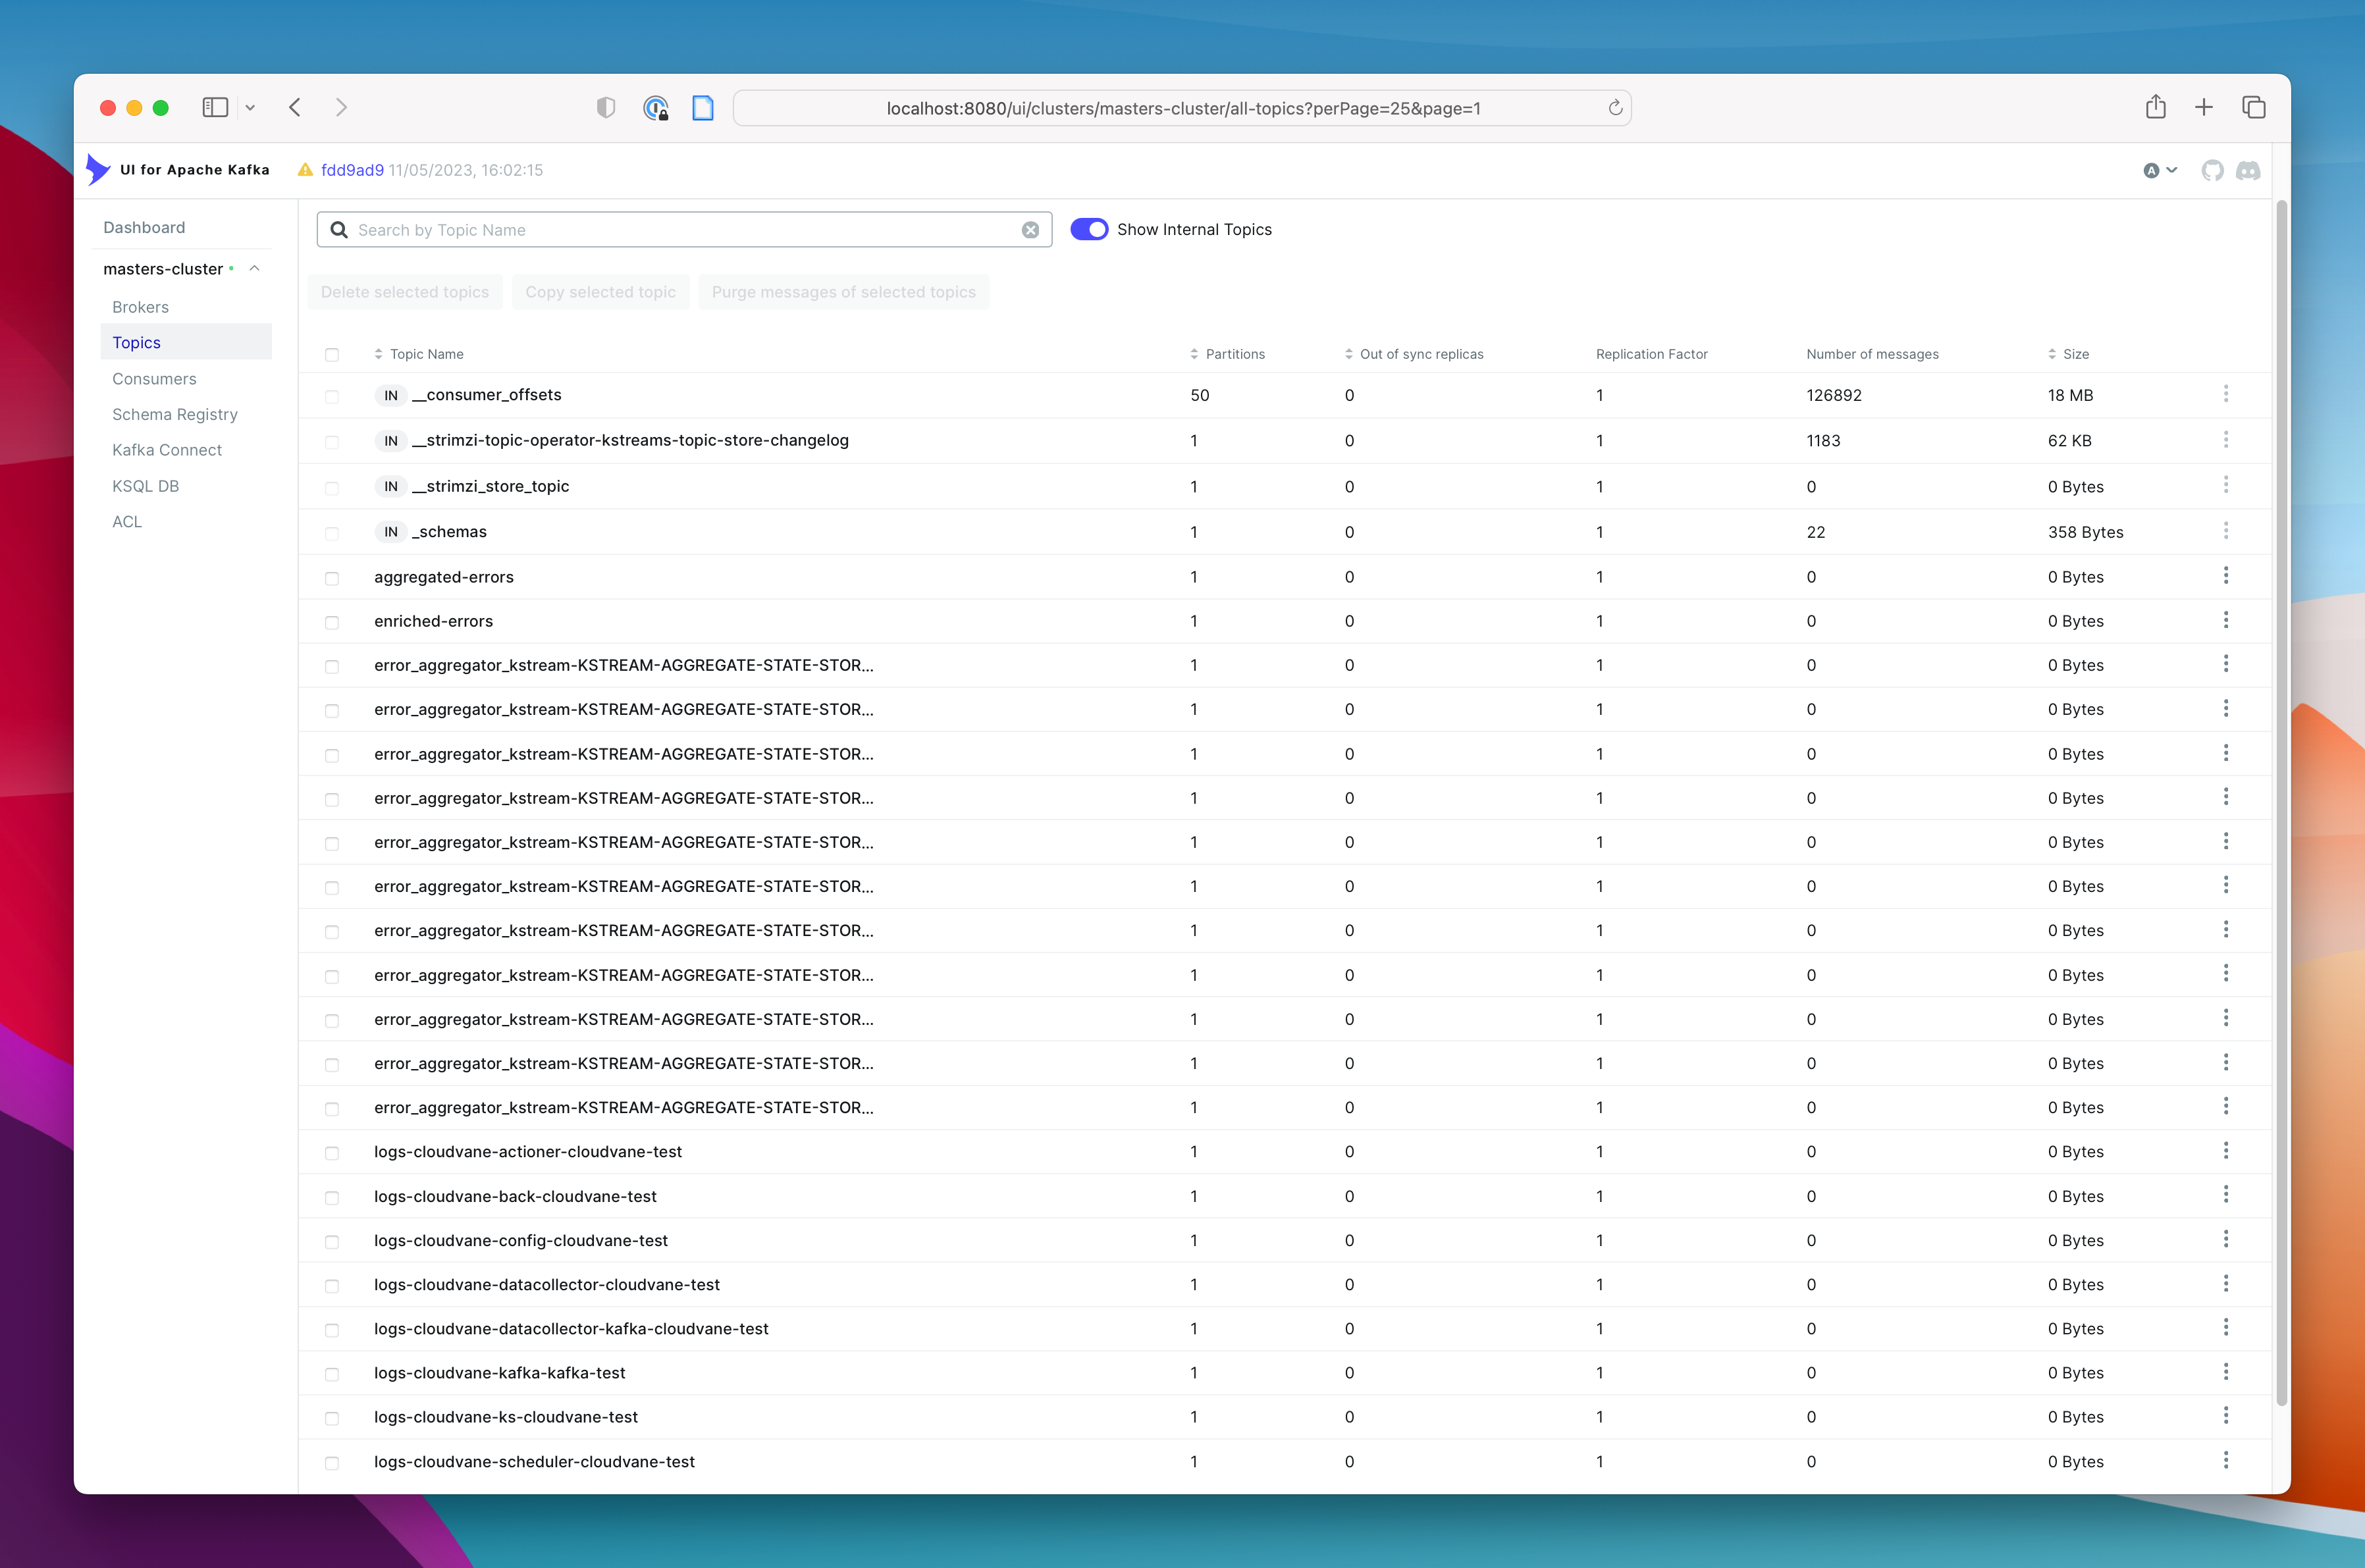
\includegraphics[width=15cm]{images/kafka-ui.png}
	\caption[Kafka teme na lokalnom Apache Kafka grozdu kroz pogled Kafka UI servisa]{Kafka teme \engl{topics} na lokalnom Apache Kafka grozdu kroz pogled Kafka UI servisa}
	\label{fig:kafkaui}
\end{figure}

Kada se podaci zabilježe u Apache Kafku, svaki konzument poruka može se povezati na relevantnu temu i čitati poruke. U okviru ovog rada, konzumenti poruka izvornih dnevničkih zapisa su Logstash i Kafka Streams aplikacija.

Kasnije u procesu, prema dijagramu toka podataka \ref{fig:topics}, vidljivo je kako se servisi za obogaćivanje i notifikacije također povezuju na određene teme kako bi čitali poruke. Servis za obogaćivanje dodatno upisuje obogaćene podatke u svoju temu. Ovaj proces omogućava dnevničkim zapisima da prođu kroz niz transformacija prije nego što se konzumiraju, pružajući tako dodatne vrijednosti.\\

Sve relevantne Kafka teme detaljno su opisane u tablici \ref{tbl:topics}, u kojoj je naveden i opis podataka koji se nalaze u svakoj od njih. Ova tablica pruža korisne informacije o tome što svaka tema predstavlja, čime olakšava razumijevanje strukture i svrhe svake teme.

\clearpage
\begin{longtblr}[
caption = {Kafka teme s dnevničkim zapisima},
label = {tbl:topics},
]{
	colspec = {X[1,l]|X[1,l]}, 
	rowhead = 1,
}
\hline
Ime Kafka teme & Sadržaj podataka u temi \\
\hline
logs-cloudvane-*-cloudvane-test & Dnevnički zapisi pojedinog CloudVane mikro-servisa \\ 
aggregated-errors & Agregirani dnevnički zapisi grešaka koje upisuje Kafka Streams aplikacija\\
enriched-errors & Agregirani dnevnički zapisi grešaka s dodatkom o potencijalnom rješenju koje upisuje Python servis koji obogaćuje poruku greške pomoću umjetne inteligencije\\
error\_aggregator\_kstream\_* & Interna tema Kafka Streams aplikacije za spremanje podataka potrebnih za agregacije\\
\_consumer\_offsets & Interna tema Apache Kafke za spremanje pozicije čitanja \\
\_schemas & Interna tema za Schema Registry servis za pohranu shema\\
\_strimzi* & Interne teme Strimzi servisa\\
\hline
	
\end{longtblr}

\section{Agregiranje dnevničkih zapisa}
\label{sec:streamImpl}

Dnevnički zapisi mogu biti itekako brojni, posebno u kompleksnim sustavima. Na primjer, u CloudVane testnom okruženju može se generirati i do $15000$ dnevničkih zapisa u samo jednom satu. Ovaj velik broj zapisa često je simptom nekog problema unutar sustava, gdje se greške javljaju i sustav započne s generiranjem obavijesti o problemima.

No, problemi se rijetko riješe sami od sebe. Sustav obično nastavlja generirati dnevničke zapise sve dok se problem ne riješi. To može rezultirati velikim količinama dnevničkih zapisa koje treba obraditi i analizirati kako bi se razumjelo što se točno događa unutar sustava.

Svaki dnevnički zapis u stanju je pružiti dragocjene informacije o različitim aspektima sustava, uključujući performanse, potencijalne greške, ponašanje korisnika i ostale vitalne elemente operativnosti sustava. No, dnevnički zapisi često sadrže poruke o greškama koje se iznimno često ponavljaju u kratkim vremenskim intervalima stvarajući time veliku količinu redundantnih informacija.\\

Upravo u ovom kontekstu \textbf{Kafka Streams} biblioteka postaje iznimno korisna. Kafka Streams, opisana u poglavlju \ref{sec:kstream}, agregiranjem sličnih ili identičnih dnevničkih zapisa može drastično smanjiti količinu podataka koju treba obraditi zadržavajući ključne informacije o greškama i problemima unutar sustava.

Na taj se način omogućuje obrada agregiranih informacija, što omogućuje brže i efikasnije identificiranje te rješavanje problema. Ovaj pristup ne samo da smanjuje kompleksnost i trošak analize dnevničkih zapisa već i olakšava otkrivanje dubljih uzoraka i trendova, omogućavajući proaktivno rješavanje problema prije nego što uzrokuju ozbiljnije posljedice.\\

Izrađena Kafka Streams aplikacija, čiji je algoritam prikazan pseudokodom \ref{algo:kstream} i čija je topologija ilustrirana na dijagramu \ref{fig:kstream}, uključuje sljedeće korake:

\begin{enumerate}
	\item Dnevnički zapisi se konzumiraju iz svih Kafka tema koje započinju ključnom riječi \emph{\glqq logs\grqq}.
	\item Dnevnički zapisi se filtriraju temeljem statusa koji određuje jesu li to informativni dnevnički zapisi ili predstavljaju greške. U ovom kontekstu izostavljaju se svi dnevnički zapisi koji ne predstavljaju greške s obzirom na to da je cilj korisniku pružiti reakciju na greške unutar aplikacije.
	\item Dnevnički zapisi grupiraju se prema ključu Kafka poruke unutar kojeg se nalazi sadržaj greške. (Ključ Kafka poruke je definiran u konfiguraciji Filebeat servisa, što je prikazano u isječku \ref{lst:filebeat})
	\item Agregacija dnevničkih zapisa provodi se po ključu poruke. Ovo grupiranje se izvodi korištenjem \emph{klizećeg prozora} u trajanju od \emph{$30$ sekundi}.
	\item Agregacija koju izravno pruža Kafka Streams biblioteka mapira se na objekt koji sadrži broj agregiranih poruka, kao i prvu dohvaćenu vremensku oznaku.
	\item Agregirani dnevnički zapisi se pohranjuju u Kafka temu \emph{\glqq aggregated-errors\grqq}.
\end{enumerate}

\begin{algorithm}
	\caption{Kafka Streams aplikacija}
	\label{algo:kstream}
	\begin{algorithmic}
		\STATE{\textbf{Ulaz:} $logs-.*$ -- regularni izraz Kafka tema koje treba agregirati.}
		\STATE{\textbf{Izlaz:} $aggregated-errors$ Kafka tema s filtriranim i agregiranim dnevničkim zapisima.}
		
		\FOR{($topic$ in $topics$)}
		
		\STATE{stream := $streamBuilder.stream(topic)$}
		\STATE{filteredStream := $stream.filter(isValidErrorMessage())$}
		\STATE{aggregatedStream := $filteredStream.groupByKey()$}
		\STATE{\hspace{50pt}$.windowedBy(SlidingWindow,30sec).aggregate()$}
		\STATE{mapped := $aggregatedStream.map(mapToResult())$}
		\STATE{mapped$.to(outputTopic)$}		

		\ENDFOR
	\end{algorithmic}
\end{algorithm}

\begin{figure}[htb]
	\centering
	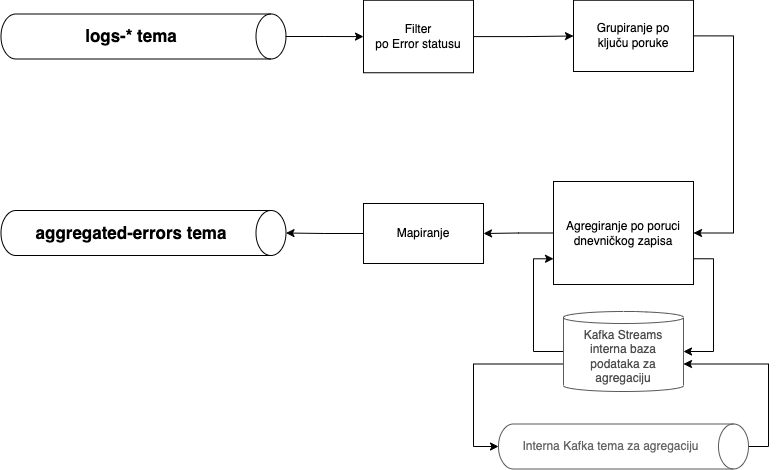
\includegraphics[width=15cm]{images/KStream.png}
	\caption[Topologija Kafka Streams aplikacije]{Topologija Kafka Streams aplikacije}
	\label{fig:kstream}
\end{figure}


\section{Obogaćivanje dnevničkih zapisa}
\label{sec:ai}

Prilikom prvog susreta s greškama unutar sustava često je nejasno u čemu je problem. Iz izravnih dnevničkih zapisa uzrok problema i njegovo potencijalno rješenje često nisu odmah očigledni.\\

U svrhu rješavanja ovog problema, ovaj rad istražuje poseban Kafka servis, izrađen u Pythonu, koji koristi \emph{OpenAI API} kako bi obogatio agregirane dnevničke zapise o greškama, a to je opisano u prethodnom poglavlju. Cilj je ovog obogaćivanja da kasnije pruži dodatne informacije korisnicima koji su zaduženi za rješavanje problema, čime se pojačava njihova sposobnost razumijevanja i brzog reagiranja na probleme.\\

Posebna značajka ovog servisa je njegova sposobnost horizontalnog skaliranja, omogućena putem Kafka Consumer API-ja. Ova karakteristika omogućuje servisu da se prilagodi povećanju opterećenja, čime se osigurava održavanje stabilnih performansi čak i pod visokim zahtjevima.\\

U procesu obogaćivanja servis koristi \emph{OpenAI API}, čiji je opis sadržan u sljedećem poglavlju, za analizu grešaka. Na temelju njegovog odgovora servis generira korisne informacije koje će korisnicima pomoći da bolje razumiju problem.

Kao što je vidljivo u dijagramu \ref{fig:topics}, ovaj servis čita dnevničke zapise iz Kafka teme \glqq \emph{aggregated-errors}\grqq, obogaćuje ih koristeći OpenAI API, a zatim ih šalje u novu Kafka temu pod nazivom \glqq \emph{enriched-errors}\grqq.

Kroz ovaj proces servis ne samo da poboljšava korisnikovo razumijevanje i reakciju na greške već i pomaže u poboljšanju ukupne kvalitete i pouzdanosti sustava.

\subsection{OpenAI API}
\label{sec:openai}

\textbf{OpenAI API} predstavlja sučelje koje omogućava pristup sofisticiranim algoritmima strojnog učenja koje je razvila organizacija \emph{OpenAI}. Ovi algoritmi sposobni su za razumijevanje, generiranje i interpretiranje prirodnog jezika, što ih čini iznimno korisnima za širok spektar primjena. U kontekstu ovog rada ti se algoritmi koriste za obogaćivanje informacija o greškama u dnevničkim zapisima.\\

Za potrebe ovog rada korišten je OpenAI model pod nazivom \emph{text-davinci-003}. No, važno je naglasiti da se prethodno opisani servis može konfigurirati za upotrebu bilo kojeg dostupnog modela OpenAI API-ja.

Model \emph{text-davinci-003} jedan je od najmoćnijih modela za obradu prirodnog jezika koje je OpenAI razvio. Ovaj model je treniran na širokom skupu podataka, što mu omogućava da razumije i generira koherentan i kontekstualno relevantan tekst temeljen na dobivenim ulaznim podacima. Takva sposobnost modela omogućuje visokokvalitetno obogaćivanje informacija sadržanih u dnevničkim zapisima.

Komunikacija s OpenAI API-jem može se ostvariti kroz HTTP protokol ili kroz biblioteke napisane za popularne programerske jezike. U ovom radu odabrana je direktna komunikacija putem HTTP protokola s OpenAI API-jem.

\section{Notifikacije u stvarnom vremenu}
\label{sec:notifService}

Problem s identifikacijom grešaka u sustavima može biti izazovan. Kada greška nastane, često nije odmah evidentno da određeni servis ima problem i da je njegov rad narušen. Ovaj izazov može otežati pravovremeno rješavanje problema, održavanje pouzdanosti i performansi sustava.\\

Kako bi se riješio ovaj problem, za potrebe rada je razvijen poseban servis. Ovaj servis također je izrađen u Pythonu i ima mogućnost horizontalnog skaliranja zahvaljujući mogućnostima koje pruža Kafka Consumer API. Ova značajka omogućuje servisu da se prilagodi promjenjivim zahtjevima za performanse, omogućujući mu da efikasno obrađuje velike količine podataka i održava visoku razinu usluge.\\

Ovaj servis služi kao sustav za obavještavanje, poslužujući se različitim kanalima kako bi korisnike obavijestio o nastalim greškama u sustavu. To se postiže slanjem notifikacija putem elektroničke pošte, objavama na Slack kanalu te slanjem obavijesti putem Pushover aplikacije. Ovaj višekanalni pristup obavještavanja osigurava da relevantne informacije o problemima dođu do korisnika na najbrži i najefikasniji mogući način.

Svaka obavijest sadrži ključne informacije o grešci, uključujući vrijeme kada je greška prvi put identificirana, opis problema prema informacijama iz dnevničkih zapisa, kao i dodatne informacije dobivene putem OpenAI API-ja. Ove informacije pomažu korisnicima da brzo shvate prirodu problema olakšavajući time proces traženja rješenja.\\

Dnevnički zapisi koji se isporučuju u notifikacijama čitaju se iz Kafka teme \emph{\glqq enriched-errors\grqq} kao što je vidljivo na dijagramu \ref{fig:topics}. Primjeri notifikacija prikazani su na sljedećim slikama: notifikacija elektroničke pošte nalazi se na slici \ref{fig:notif_email}, Slack notifikacija na slici \ref{fig:notif_slack}, a Pushover mobilna notifikacija na slici \ref{fig:notif_pushover}.

\begin{figure}[htb]
	\centering
	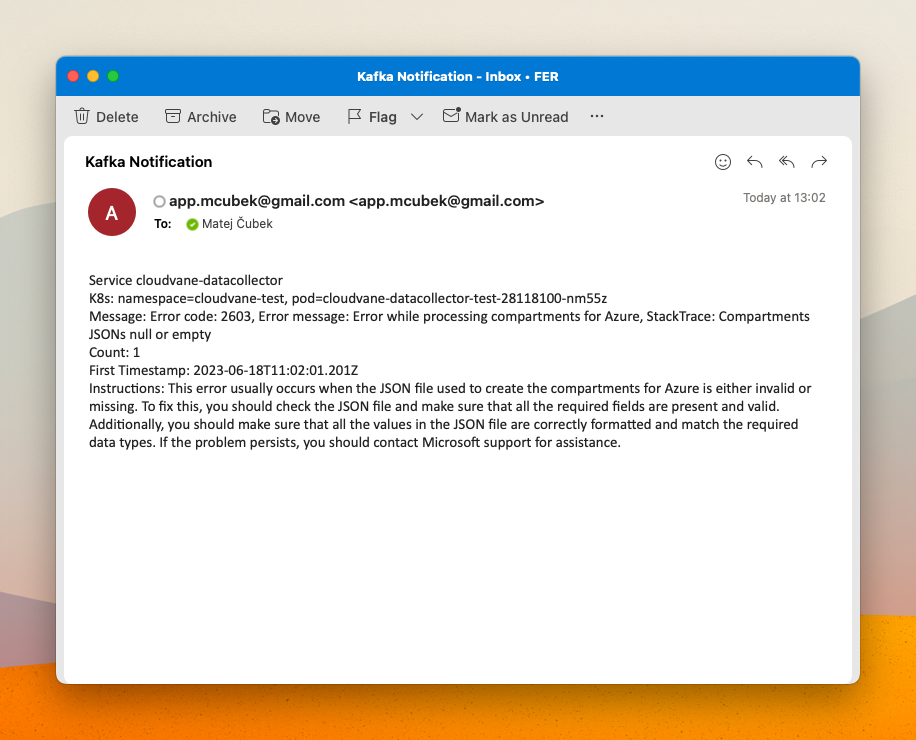
\includegraphics[width=12cm]{images/email_notif.png}
	\caption[Primjer notifikacije dnevničkog zapisa greške kroz elektroničku poštu]{Primjer notifikacije dnevničkog zapisa greške putem elektroničke pošte}
	\label{fig:notif_email}
\end{figure}

\begin{figure}[htb]
	\centering
	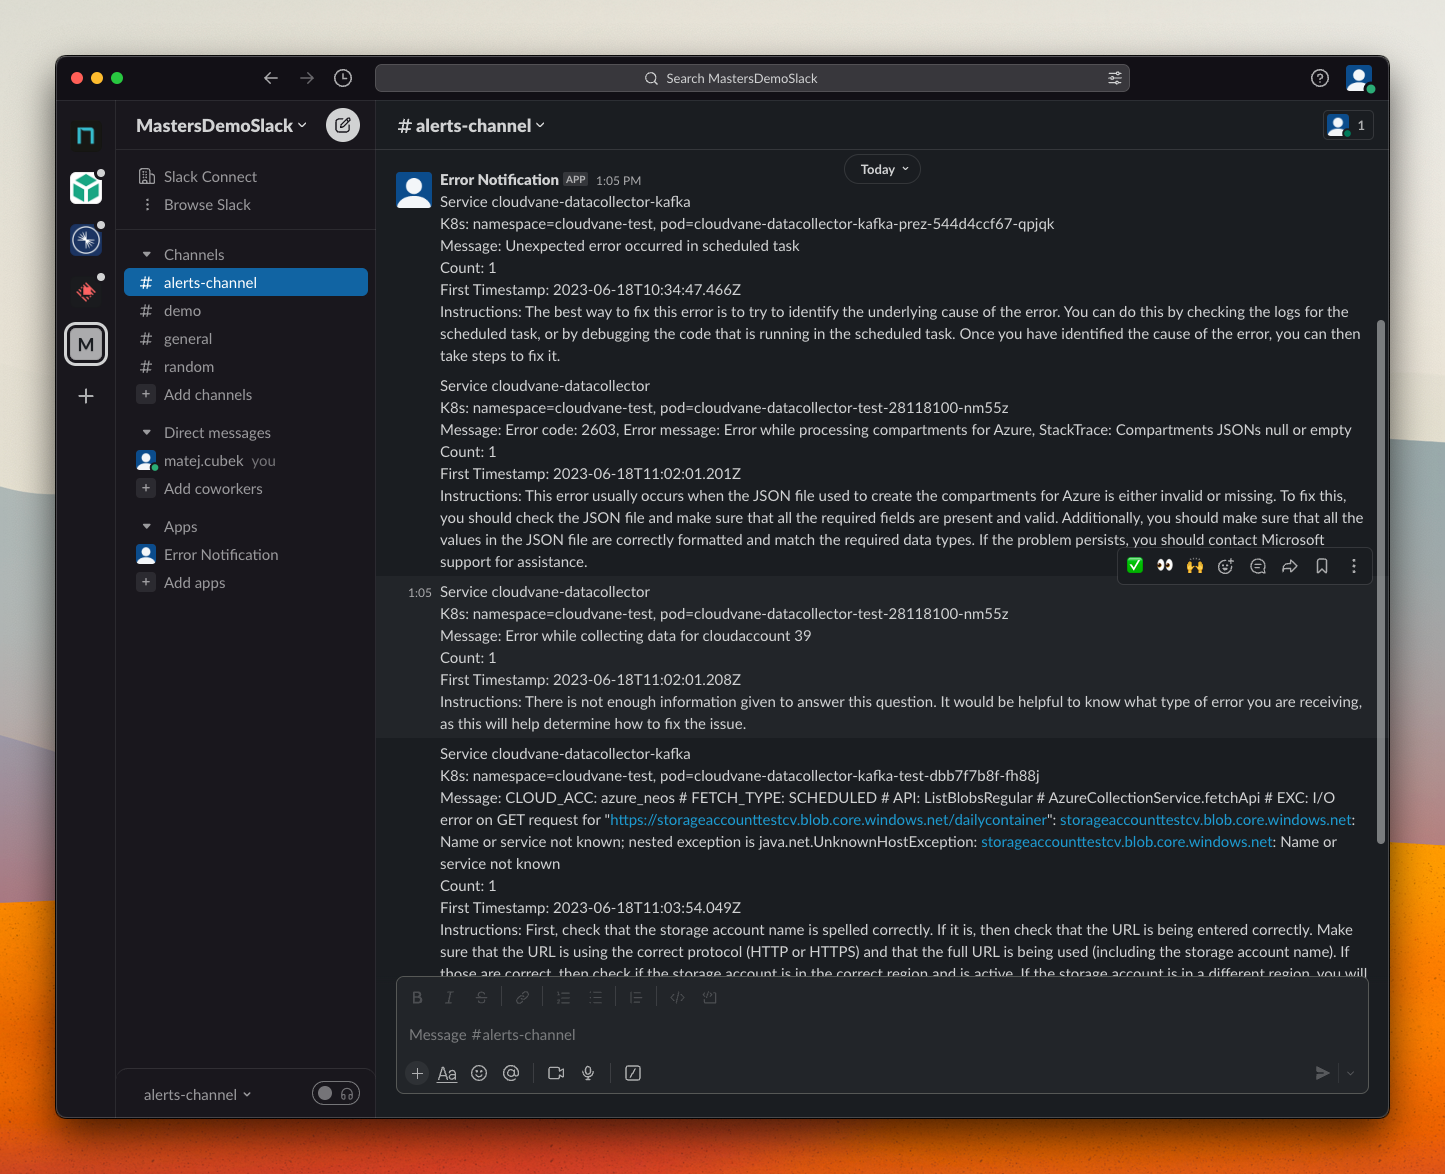
\includegraphics[width=14cm]{images/slack_notif.png}
	\caption[Primjer notifikacije dnevničkog zapisa greške putem Slack aplikacije]{Primjer notifikacije dnevničkog zapisa greške putem Slack aplikacije}
	\label{fig:notif_slack}
\end{figure}

\begin{figure}[htb]
	\centering
	
\includegraphics[width=6cm]{images/mobile_notif.png}
	\caption[Primjer notifikacije dnevničkog zapisa greške putem Pushover mobilne aplikacije]{Primjer notifikacije dnevničkog zapisa greške putem Pushover mobilne aplikacije}
	\label{fig:notif_pushover}
\end{figure}

Ovaj servis je ključan za održavanje stabilnosti sustava omogućavajući pravovremeno reagiranje na greške, smanjenje vremena neaktivnosti i poboljšanje ukupne kvalitete usluge.

\clearpage
\section{Pregled kroz Kibanu}
\label{sec:kibanaImpl}

Naposljetku, ako dođe do greške u aplikaciji i treba ju popraviti, potrebno je pregledati stanja svih servisa. Pregled stanja servisa u većini slučajeva uključuje pregled dnevničkih zapisa, međutim to, kao što je prethodno opisano, u distribuiranoj okolini nije jednostavan zadatak. Zbog velikog broja servisa za potpun pregled sustava potrebno je koristiti alat poput Kibane koji agregira dnevničke zapise \engl{logs}, a uvod u nju dan je u poglavlju \ref{sec:kibana}.\\

Kibana, sučelje podataka ElasticSearch-a, omogućuje pregled dnevničkih zapisa svih servisa sustava kroz objedinjeno sučelje i omogućuje njihovo filtriranje po svim dostupnim atributima poput čvora grozda, imena servisa, prostora imena itd., kao što je prikazano na slici \ref{fig:kibana-filter}.

\begin{figure}[htb]
	\centering
	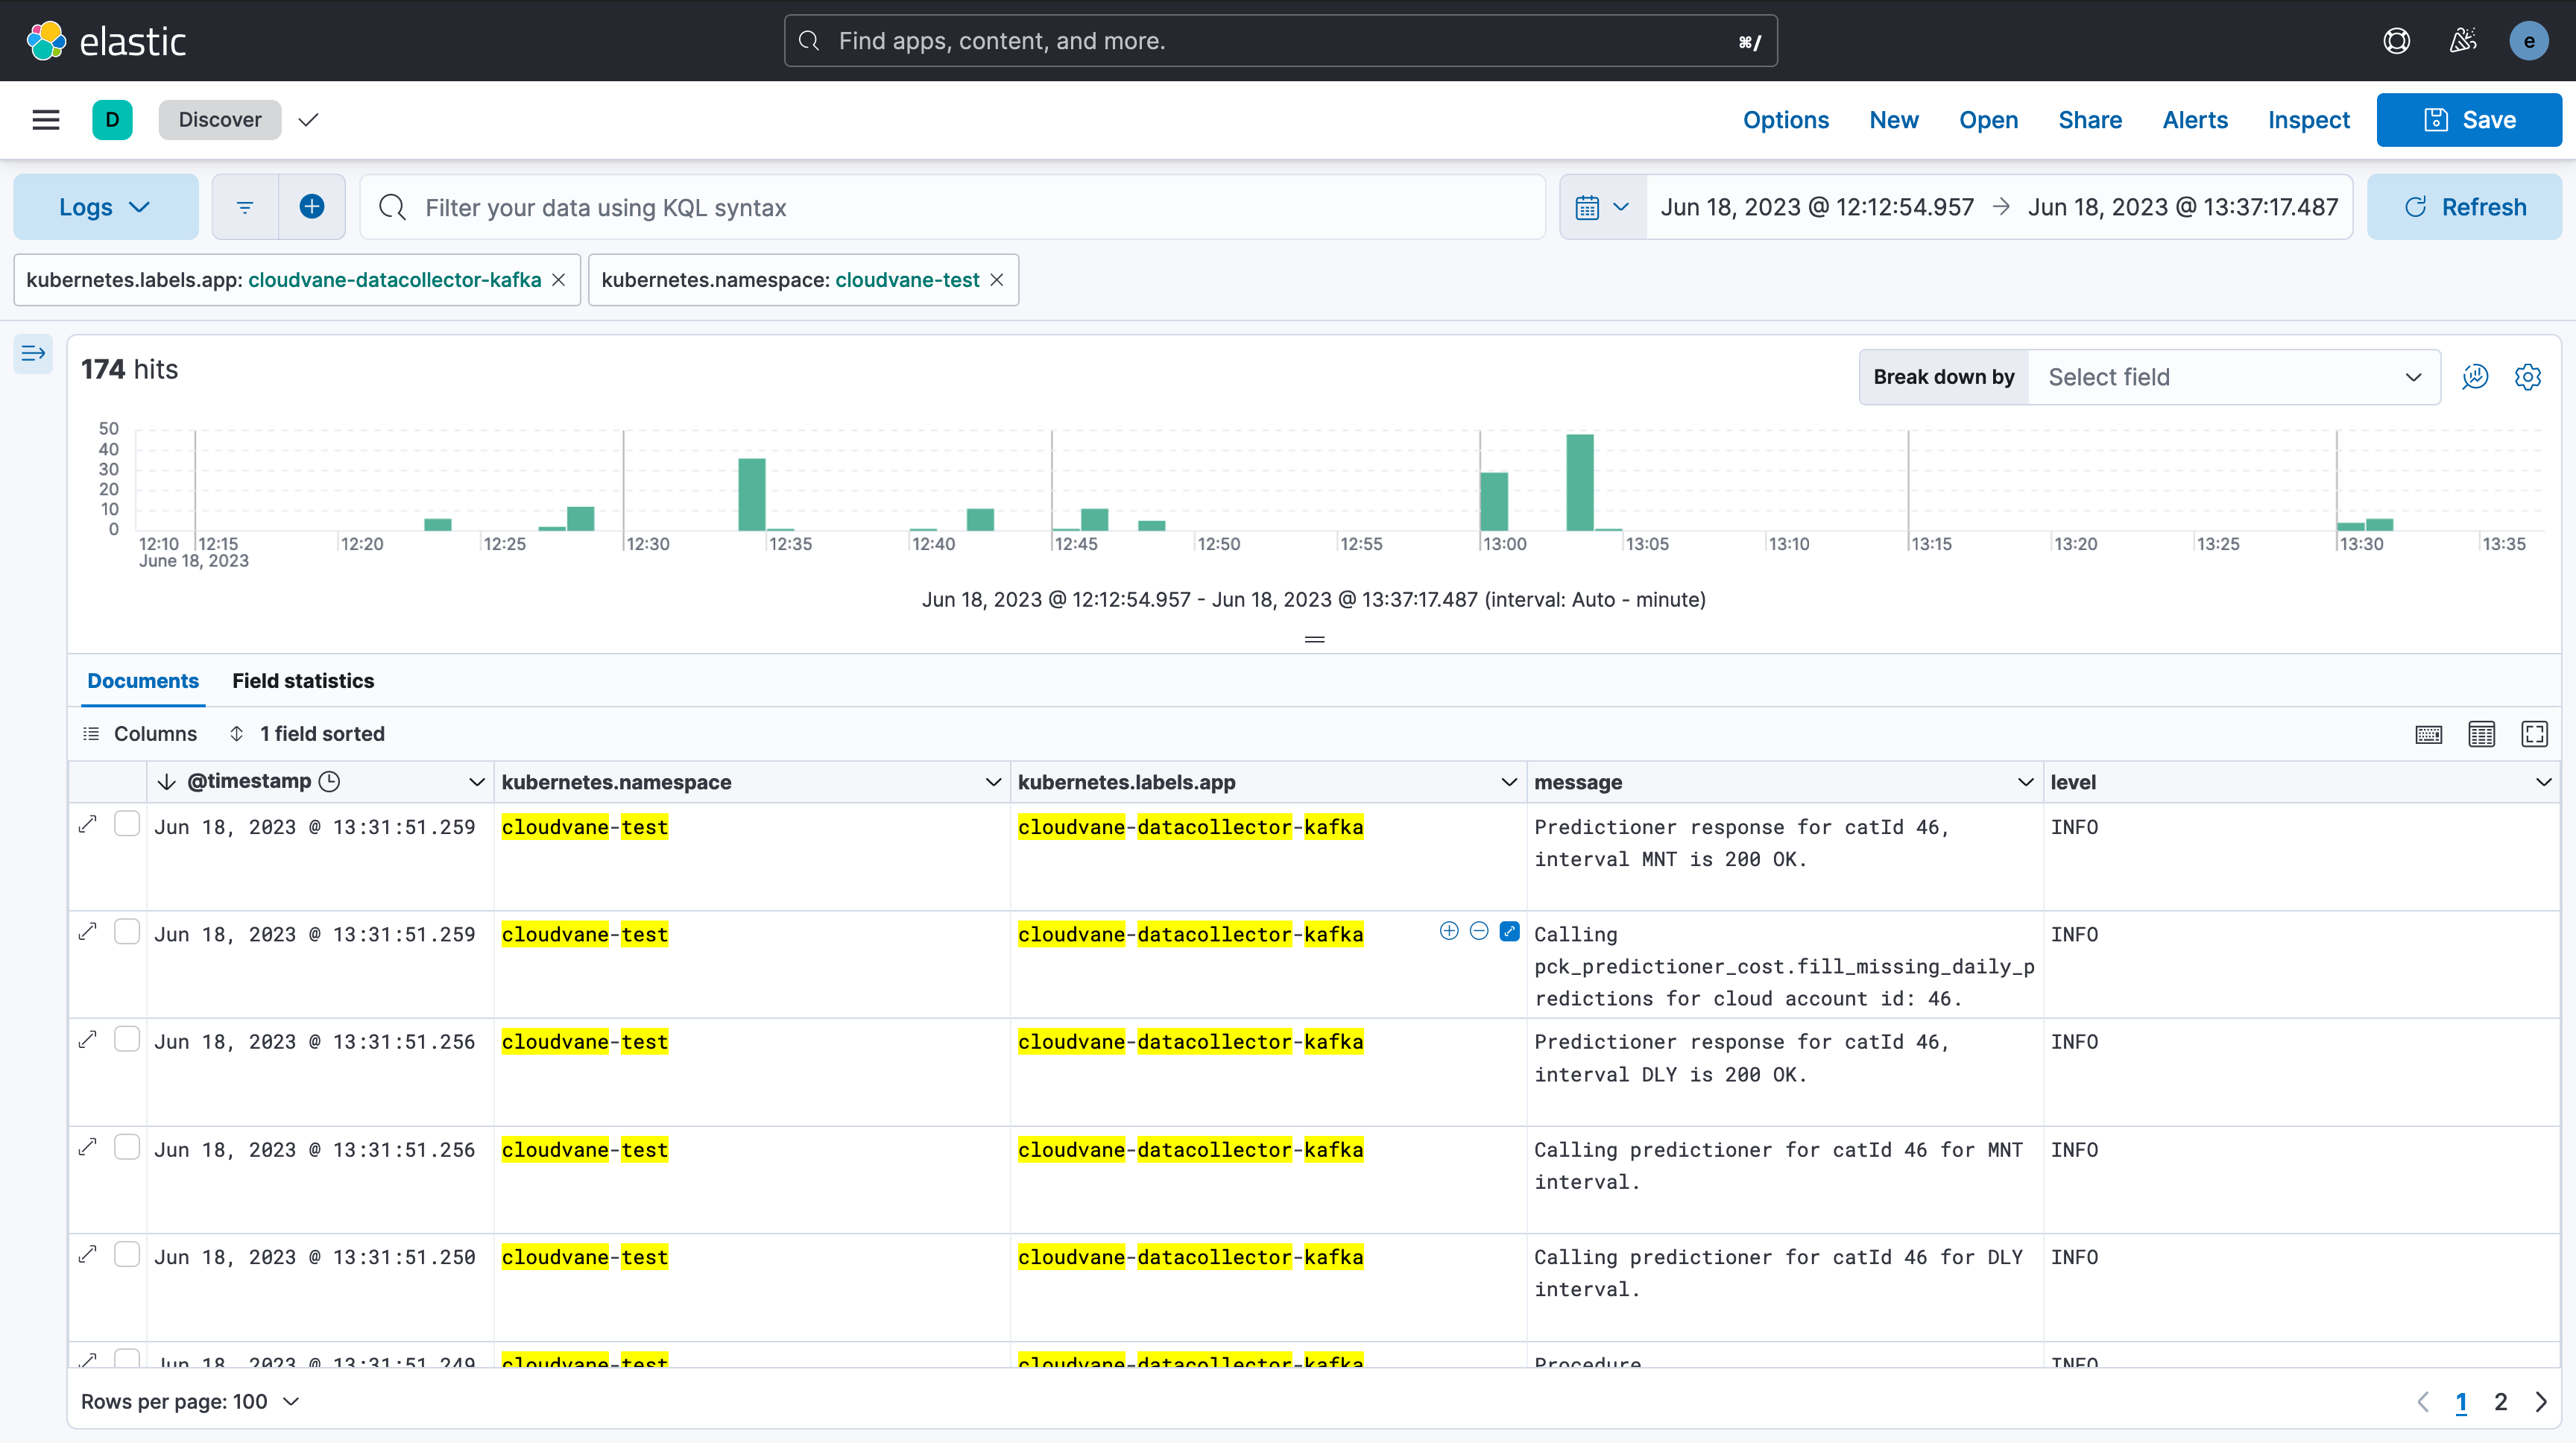
\includegraphics[width=15cm]{images/kibana-filter.png}
	\caption[Prikaz filtriranih dnevničkih zapisa u Kibana sučelju]{Prikaz filtriranih dnevničkih zapisa \engl{logs} u Kibana sučelju}
	\label{fig:kibana-filter}
\end{figure}

Kibana također omogućuje i kreiranje kontrolnih ploča s ključnim metrikama kao što je prikazano na slici \ref{fig:kibana-dash}. Ove kontrolne ploče pružaju brzi pregled performansi i stanja sustava te mogu pomoći u brzom identificiranju i rješavanju problema.

\begin{figure}[htb]
	\centering
	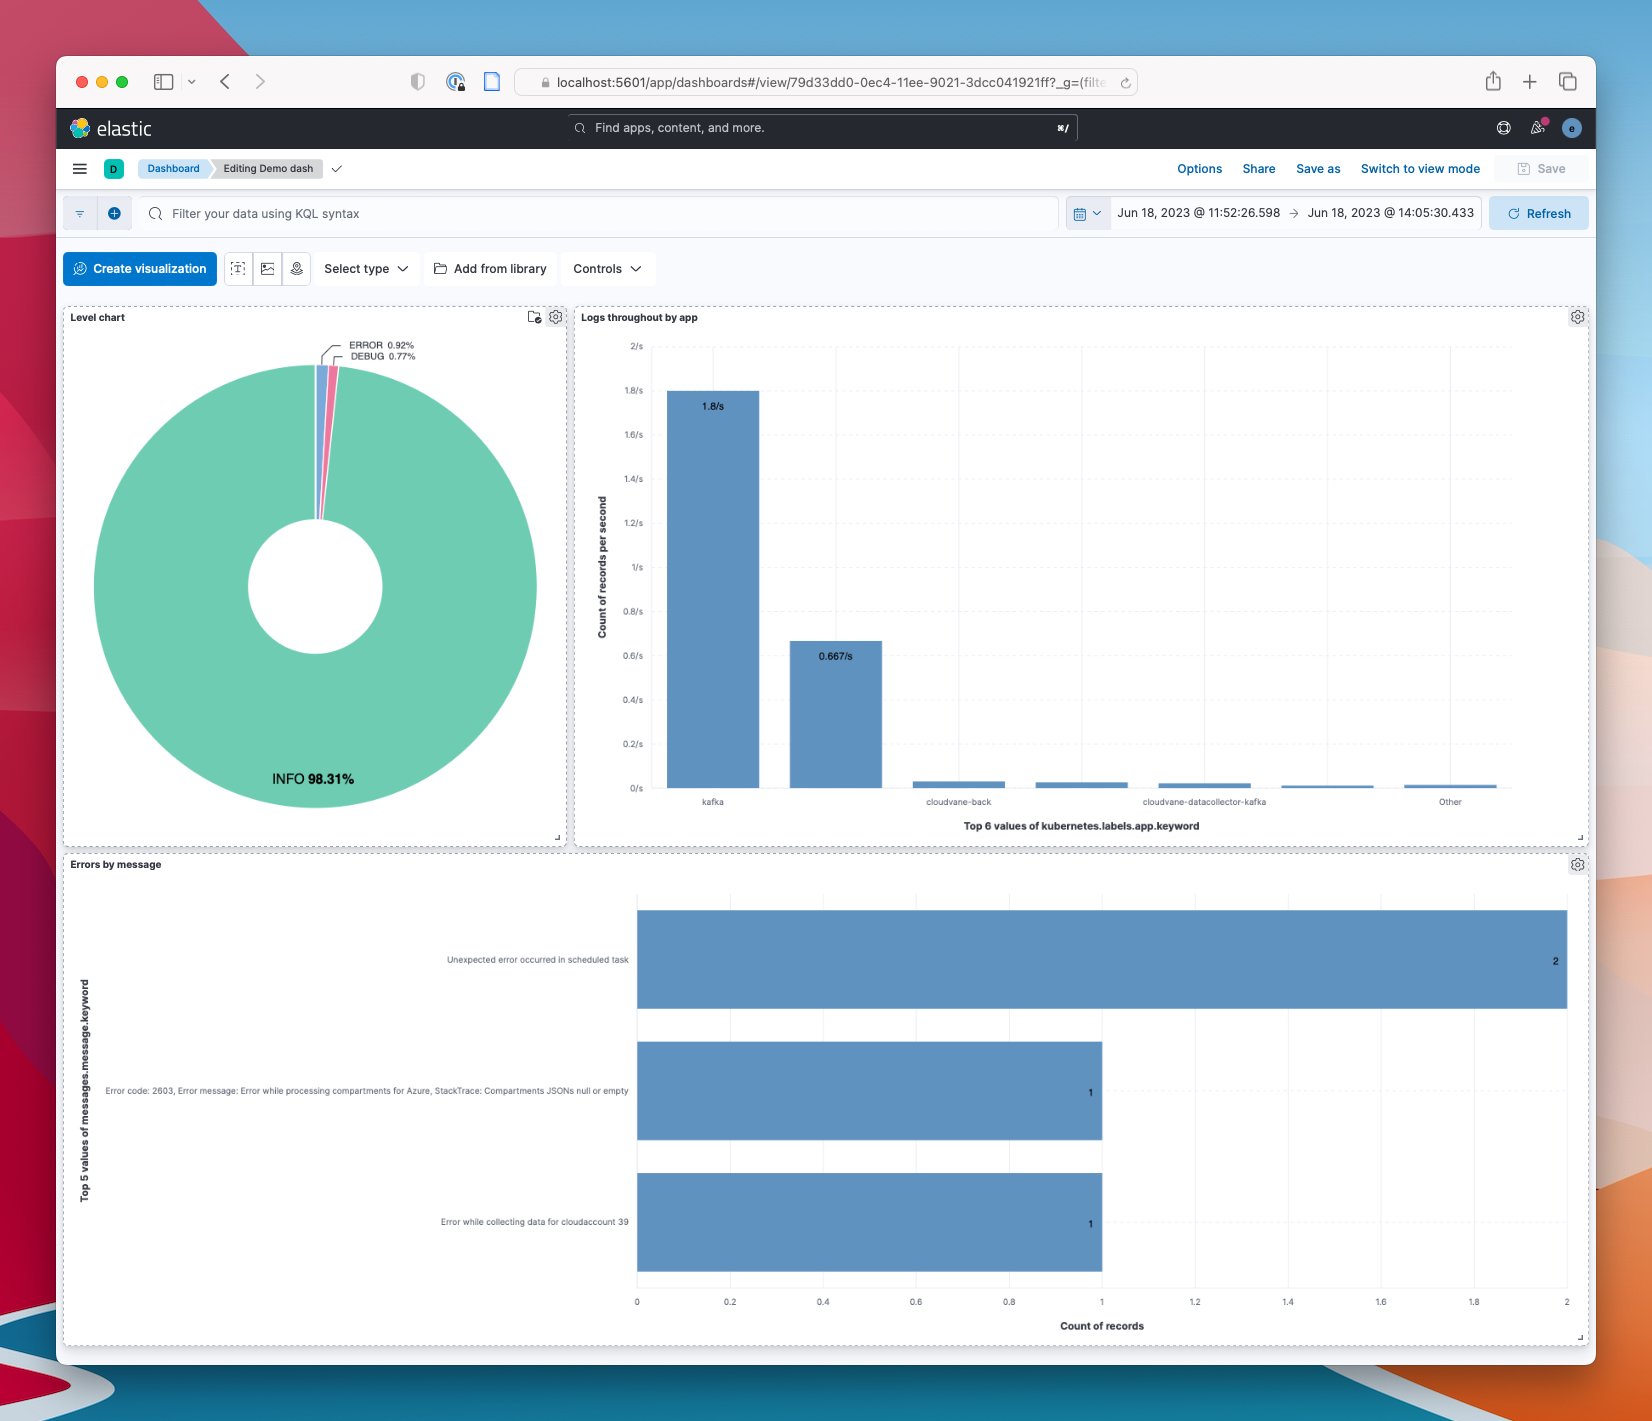
\includegraphics[width=15cm]{images/kibana-dash.png}
	\caption[Prikaz kreirane kontrolne ploče u Kibani]{Prikaz kreirane kontrolne ploče u Kibani}
	\label{fig:kibana-dash}
\end{figure}

\chapter{Zaključak}
\label{sec:conclusion}

U doba digitalizacije i sve veće ovisnosti o informacijskim sustavima efikasno i pravovremeno praćenje dnevničkih zapisa postaje presudno za pravilan rad i održavanje aplikacija. U ovom radu prikazano je istraživanje kako se platforme \emph{Apache Kafka} i \emph{ELK}, uz pomoć \emph{OpenAI API-ja}, mogu iskoristiti za obradu i analizu dnevničkih zapisa raspodijeljenih sustava u stvarnom vremenu.

ELK platforma koja uključuje \emph{ElasticSearch}, \emph{Logstash} i \emph{Kibanu}, zajedno s Apache Kafka platformom koristila se za obradu, prikupljanje i prikaz dnevničkih zapisa. \emph{Kafka Streams} biblioteka korištena je za agregaciju dnevničkih zapisa, a OpenAI API za obogaćivanje zapisa, što omogućuje dublju analizu i razumijevanje informacija prikupljenih iz sustava.

Na primjeru SaaS aplikacije \emph{CloudVane} tvrtke \emph{Neos} demonstriralo se kako je moguće primijeniti opisane metode i tehnologije za nadzor dnevničkih zapisa u složenim distribuiranim sustavima. Rezultati istraživanja pokazali su da je korištenjem navedenih alata moguće detektirati i nadzirati anomalije u radu sustava na učinkovit način.

Rad je također pokazao kako se korištenjem Apache Kafka platforme i ELK platforme mogu unaprijediti pouzdanost i brzina obrade podataka, što omogućuje pravovremeno reagiranje i pregled problema sustava.\\

Nadalje, kao nastavak na ovaj rad otvaraju se mogućnosti za buduća istraživanja. Primjerice, moguće je izgraditi servis koji bi, ovisno o detektiranoj grešci na koju je pretplaćen, mogao pokrenuti odgovarajuću skriptu. Moguće je integrirati servis \emph{Grafana} za vizualizaciju sustava. Također, postoji prostor za poboljšanje postojećih procesa, unapređenje automatizacije te ugradnju modela predikcije koji bi mogao koristiti kontekst prošlih pojavljenih dnevničkih zapisa.

\bibliography{literatura}
\bibliographystyle{fer}


\lstset{
	aboveskip=3mm,
	belowskip=3mm,
	showstringspaces=false,
	columns=flexible,
	basicstyle={\small\ttfamily},
	numbers=none,
	numberstyle=\tiny\color{gray},
	keywordstyle=\color{blue},
	commentstyle=\color{dkgreen},
	stringstyle=\color{mauve},
	breaklines=true,
	breakatwhitespace=true,
	tabsize=3
}


\appendix
\chapter{Isječci programskog koda}
\label{sec:code}


\begin{lstlisting}[caption={Primjer dnevničkog zapisa CloudVane servisa}
		,label={lst:cloudvaneLog}
		,language=json]
{
	"@timestamp": "2023-06-11T20:32:51.032Z",
	"@version": "1",
	"message": "Calling data_collector.prepare_cost_history for cloud account id: 76.",
	"logger_name": "hr.neos.cloudvane.datacollector.predictioner. PredictionerService",
	"thread_name": "scheduling-1",
	"level": "INFO",
	"level_value": 20000
}
\end{lstlisting}

\clearpage
\begin{lstlisting}[caption={Konfiguracija Logback-a}
	,label={lst:logback_xml}
	,language=XML]
<?xml version="1.0" encoding="UTF-8"?>
<configuration>
<contextName>cloudvane-dc-kafka</contextName>

<!-- Include CONSOLE_LOG_PATTERN -->
<include resource="org/springframework/boot/logging/logback/defaults.xml"/>

<appender name="CONSOLE_PATTERN" class="ch.qos.logback.core.ConsoleAppender">
<layout class="ch.qos.logback.classic.PatternLayout">
<Pattern>${CONSOLE_LOG_PATTERN}</Pattern>
</layout>
</appender>

<appender name="CONSOLE_JSON" class="ch.qos.logback.core.ConsoleAppender">
<encoder class="net.logstash.logback.encoder.LogstashEncoder" />
</appender>

<springProfile name="local">
<root level="INFO">
<appender-ref ref="CONSOLE_PATTERN" />
</root>
</springProfile>

<springProfile name="dev,dev-test,test,prod">
<root level="INFO">
<appender-ref ref="CONSOLE_JSON" />
</root>
</springProfile>
</configuration>
\end{lstlisting}

\clearpage
\begin{lstlisting}[caption={Primjer dnevničkog zapisa sa CloudVane servisa s metapodacima}
		,label={lst:cloudvaneLog}
		,language=json]
{
	"@timestamp": "2023-05-03T17:00:04.068Z",
	"@metadata": {
		"beat": "filebeat",
		"type": "_doc",
		"version": "8.7.1"
	},
	"log": {
		"offset": 294991,
		"file": {
			"path": "/var/log/containers/cloudvane-datacollector..."
		}
	},
	"level_value": 20000,
	"logger_name": "hr.neos.cloudvane.datacollector.collector.cloud.azure.
	AzureCollectionService",
	"ecs": {
		"version": "8.0.0"
	},
	"host": {
		"ip": [
		"10.244.1.90",
		"fe80::8bf:80ff:fe5f:3832"
		],
		"mac": [
		"0A-BF-80-5F-38-32"
		],
		"hostname": "filebeat-kafka-matej-44gl2",
		"architecture": "x86_64",
		"os": {},
		"containerized": true,
		"name": "filebeat-kafka-matej-44gl2"
	},
	"stream": "stdout",
	"input": {
		"type": "container"
	},
	"instana.trace.id": "adf2108f84007f73",
	"level": "INFO",
	"container": {
		"id": "a248de8e52ca95d0591cd220cd4f
		438488e4765bc1de51644c4c7621784b9e45",
		"runtime": "cri-o",
		"image": {
			"name": "fra.ocir.io/frpf7jvyycgx/cv-kafka/openjdk-17/
			cloudvane-datacollector:1fc43..."
		}
	},
	"message": "Fetching AZURE cost file list from URL: 
	https://storageaccounttestcv.blob.core.windows.net/
	dailycontainer?restype=container&comp=list",
	"agent": {
		"ephemeral_id": "5c71c9f5-3073-4b71-90a8-04ef13492db4",
		"id": "18a62338-ce41-4a14-9d6d-e9f6887041b0",
		"name": "filebeat-kafka-matej-44gl2",
		"type": "filebeat",
		"version": "8.7.1"
	},
	"@version": "1",
	"thread_name": "scheduling-1",
	"kubernetes": {
		"labels": {
			"app": "cloudvane-datacollector-kafka",
			"client": "test",
			"pod-template-hash": "75f86b6d7c"
		},
		"container": {
			"name": "cloudvane-datacollector"
		},
		"node": {
			"labels": {	},
			"hostname": "10.38.1.11",
			"name": "10.38.1.11",
			"uid": "9c999e81-cafc-405c-936c-8c45183351b5"
		},
		"pod": {
			"ip": "10.244.1.5",
			"name": "cloudvane-datacollector-kafka-test-75f86b6d7c-g2kgb",
			"uid": "1a2ff384-ac41-47d0-815d-43c27591cff7"
		},
		"namespace": "cloudvane-test",
		"namespace_uid": "4af72ed8-18a8-4d35-ad03-966d1804e9c7",
		"namespace_labels": {
			"kubernetes_io/metadata_name": "cloudvane-test"
		},
		"replicaset": {
			"name": "cloudvane-datacollector-kafka-test-75f86b6d7c"
		}
	},
	"indexName": "cloudvane-datacollector-kafka"
}
\end{lstlisting}

\clearpage
\begin{lstlisting}[caption={Konfiguacija Logstash-a na lokalnom Kubernetes grozdu}
	,label={lst:logstash}]
input {
	kafka {
		bootstrap_servers => "masters-cluster-kafka-bootstrap.kafka.svc.cluster.local:9092"
		topics_pattern => "^logs.*"
		group_id => "logstash"
		codec => "json"
		decorate_events => "extended"
	}
}
filter {
	mutate {
		add_field => { "topic" => "%{[@metadata][kafka][topic]}" }
	}
}
output {
	elasticsearch {
		
		hosts => ["https://masters-es-internal-http.elk.svc.cluster.local:9200"]
		index => "k8s-%{topic}"
		
		ssl => true
		ssl_certificate_verification => false
		user => "elastic"
		password => "ELASTIC_PASSWORD"
		
		ilm_enabled => false
	}
}
\end{lstlisting}

\clearpage
\begin{lstlisting}[caption={Konfiguacija Filebeat-a na CloudVane Kubernetes grozdu}
	,label={lst:filebeat}
	,language=yaml]
filebeat.inputs:
- type: container
format: cri
paths:
- /var/log/containers/*.log
processors:
- decode_json_fields:
fields: [ "message" ]
target: ""
overwrite_keys: true
- add_kubernetes_metadata:
in_cluster: true
host: ${NODE_NAME}
matchers:
- logs_path:
logs_path: /var/log/containers/
- script:
lang: javascript
source: >
function process(event) {
	var appName=event.Get("kubernetes.labels.app");
	if (appName!==null && appName.indexOf("cloudvane") !== -1)
	{
		event.Put("indexName",event.Get("kubernetes.labels.app"));
	}
	else if (appName!==null && appName.indexOf("kafka")!== -1)
	{
		event.Put("indexName","cloudvane-".concat(event.Get("kubernetes.labels.app")));
	}
	else
	{
		event.Put("indexName","other");
	}
	var input = event.Get("message");
	input = input.replace(/RequestId:[^ ]*/g, "");
	input = input.replace(/Time:[^ ]*/g, "");
	input = input.replace(/\d{4}-\d{2}-\d{2} \d{2}:\d{2}:\d{2}\.\d{3}/g, "");
	input = input.replace(/\d{4}-\d{2}-\d{2} \d{2}:\d{2}:\d{2},\d{3}/g, "");
	var kafkaKey = {
		"message": input,
		"service": event.Get("indexName"),
		"kubernetes": {
			"namespace": event.Get("kubernetes.namespace"),
			"pod": event.Get("kubernetes.pod.name")
		}
	};
	event.Put("kafkaKey", JSON.stringify(kafkaKey));
}    
- drop_event:
when:
not:
or:
- equals:
kubernetes.namespace: "cloudvane-test"
- equals:
kubernetes.namespace: "kafka-test"
- type: log
paths:
- /var/log/containers/*.out
processors:
- decode_json_fields:
fields: [ "message" ]
target: ""
overwrite_keys: true
- script:
lang: javascript
source: >
function process(event) {
	event.Put("indexName","usage");
	var kafkaKey = {
		"message": event.Get("message"),
		"service": event.Get("indexName"),
	};
	event.Put("kafkaKey", JSON.stringify(kafkaKey));
}
processors:
- add_host_metadata:
setup.template:
name: k8s
pattern: k8s-*
setup.ilm.enabled: false
output.kafka:
hosts: [ "MY_PUBLIC_IP:30096" ]
version: '2.6.0'
key: '%{[kafkaKey]}'
topic: 'logs-%{[indexName]}-%{[kubernetes.namespace]}'
partition.round_robin:
reachable_only: false
required_acks: 1
batch.max_events: 2048
compression: snappy
max_message_bytes: 1000000
ssl.enabled: true
ssl.certificate_authorities: [ '/etc/filebeat/ssl/ca.pem' ]
ssl.certificate: '/etc/filebeat/ssl/certificate.pem'
ssl.key: '/etc/filebeat/ssl/key.pem'
\end{lstlisting}

\clearpage
\begin{lstlisting}[caption={Dockerfile Kafka Streams aplikacije}
	,label={lst:streamsDockerfile}]
FROM openjdk:17
LABEL authors="matejc"

ENV PROFILE=local

WORKDIR /app
COPY build/libs/error_aggregator_stream-1.0.0.jar /app/log_aggregation_kstream.jar

EXPOSE 8080

ENTRYPOINT ["java", "-jar","-Dspring.profiles.active=${PROFILE}" ,"/app/log_aggregation_kstream.jar"]

USER 1002
\end{lstlisting}




\begin{sazetak}
U radu naslovljenom \glqq Analiza dnevničkih zapisa raspodijeljenih sustava u stvarnom vremenu\grqq\hspace{1pt} istražene su mogućnosti Apache Kafka platforme i komponenti ELK-a (ElasticSearch, Logstash i Kibana) za obradu i analizu dnevničkih zapisa raspodijeljenih mikro-servisnih aplikacija koje se izvode na Kubernetesu u stvarnom vremenu. Rad koristi OpenAI API za obogaćivanje dnevničkih zapisa s dodatnim kontekstom i informacijama. Implementirani su mehanizmi za stvarno-vremenske notifikacije i agregaciju dnevničkih zapisa koristeći Kafka Streams, što omogućuje pravovremeno otkrivanje i reagiranje na anomalije u sustavu. Korištenjem SaaS aplikacije CloudVane tvrtke Neos kao primjera, pokazano je kako se ove tehnologije mogu primijeniti u nadzoru dnevničkih zapisa u složenim distribuiranim sustavima. Ovaj rad naglašava važnost dnevničkih zapisa za otkrivanje anomalija i nadzor performansi te ulogu Apache Kafka i ELK platforme u tom kontekstu.

\kljucnerijeci{Kubernetes, Apache Kafka, Tokovi Podataka, Dnevnički zapisi, Obrada u stvarnom vremenu, Elastic, ELK, Nadzor aplikacija, Grozd računala, Logstash, Filebeat, ElasticSearch, Kibana, Minikube, Oblak}
\end{sazetak}

\clearpage
\engtitle{Real-Time Log Analysis for Monitoring Distributed Systems}
\begin{abstract}
In the thesis titled \glqq Real-time Log Analysis of Distributed Systems\grqq, the potential of Apache Kafka platform and ELK stack components (ElasticSearch, Logstash, and Kibana) for real-time processing and analysis of distributed microservice applications running on Kubernetes was explored. The study utilizes the OpenAI API for enriching log files with additional context and information. The thesis introduces mechanisms for real-time notifications and log aggregations using Kafka Streams enabling timely detection and response to system anomalies. Using Neos's SaaS application CloudVane as an example, the study demonstrates how these technologies can be implemented in monitoring log files in complex distributed systems. This work emphasizes the importance of log files for anomaly detection and performance monitoring, as well as the role of Apache Kafka and ELK platforms in this context.

\keywords{Kubernetes, Apache Kafka, Streaming, Real-Time, Logs, Elastic, ELK, Monitoring, Cluster, Logstash, Filebeat, ElasticSearch, Kibana, Minikube, Cloud}
\end{abstract} 

\end{document}
